\documentclass[10pt]{article}
\usepackage[a4paper,margin=19mm]{geometry}
\usepackage{amsmath,amssymb,mathtools,amsthm,mathrsfs,longtable,booktabs,array,calc,enumitem,float,graphicx,needspace}
\usepackage[hidelinks,hypertexnames=false]{hyperref}\usepackage{xurl}
\usepackage{fontspec}\setmainfont{DejaVu Serif}
\setlength{\emergencystretch}{4em}\providecommand{\tightlist}{}
\setcounter{secnumdepth}{0}\allowdisplaybreaks
\newtheorem{theorem}{Theorem}[section]
\newtheorem{lemma}[theorem]{Lemma}
\newtheorem{proposition}[theorem]{Proposition}
\newtheorem{corollary}[theorem]{Corollary}
\newcommand{\C}{\mathbb C}\newcommand{\Pp}{\mathcal P}
\newcommand{\Rr}{\mathcal R}\newcommand{\tr}{\operatorname{Tr}}
\newcommand{\remm}{\operatorname{rem}}\newcommand{\rank}{\operatorname{rank}}
\newcommand{\diag}{\operatorname{diag}}\newcommand{\eps}{\varepsilon}
\newcommand{\Id}{I}\newcommand{\norm}[1]{\left\lVert#1\right\rVert}
\title{Original arithmetic current and effective cutoff control\\Complete source increments, observed evolution, and hidden return}
\author{Split-Zero research programme}
\date{22 September 2026\\SZ-20260922-026}
\begin{document}\maketitle
The original kernel-volume profile and the first-order arithmetic-current
profile are connected by the exact identity
\[
J'(t)=2\psi(t)-2(1+t)\psi'(t).
\]
This edition proves a finite reconstruction from the actual source increments,
sharper complete-kernel localization and local source-window bounds, and
the original observed current's two signed directions. It calculates both
extreme singular values of the compressed arithmetic evolution and its
exact relation to the full evolution through the hidden kernel.

Both incoming manuscripts are printed in full, followed or preceded by the
complete independent derivations that strengthen them. All original cutoffs,
source minima, invariant rows, physical coordinates and mixed blocks are
retained. The earlier complete mathematical source collection accompanies
this reader as an unchanged byte prefix plus new sources.

The fixed-data simple-quartet domain is retained throughout. RC35--44 applies
the earlier conductor theorem on its proved period domain: the terminal
eigenclass has subexponential normalized current and exponentially balanced
weights in the two observed sign sectors. Its residual individual sign is
still governed by the exact complex pairing RC32. These results do not establish RH.
\begingroup\small\tableofcontents\endgroup\clearpage
\section*{The two profiles and the actual hidden return}
\addcontentsline{toc}{section}{The two profiles and the actual hidden return}
\begin{figure}[H]\centering
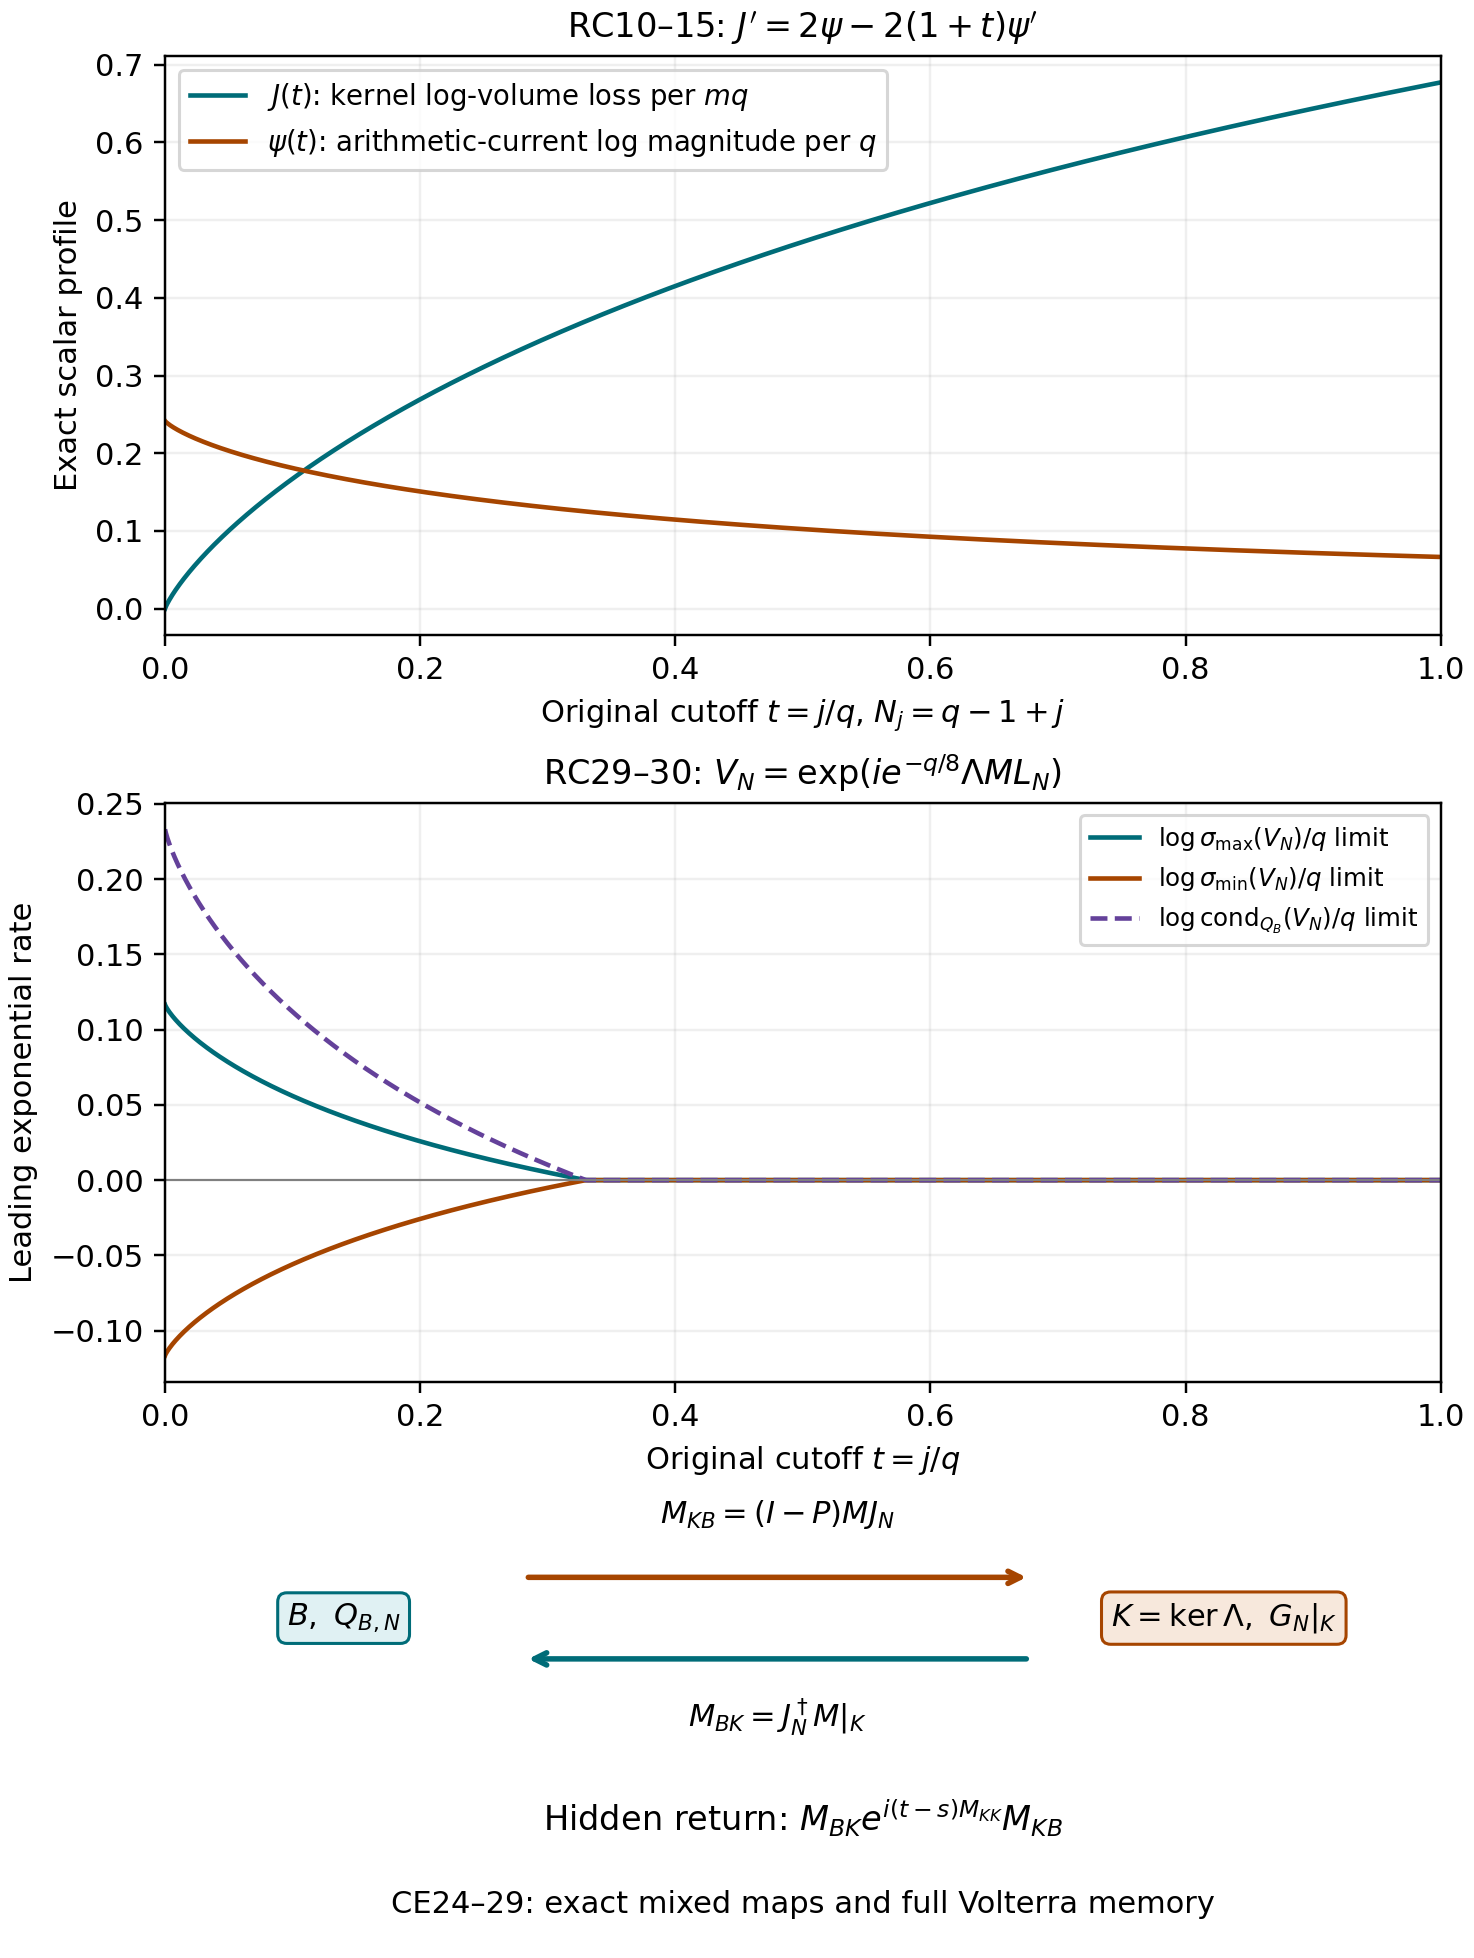
\includegraphics[width=\textwidth,height=.75\textheight,keepaspectratio]{CURRENT_CONNECTIONS.png}
\caption{Top: the two evaluated profiles in their original cutoff coordinate.
RC10--15 proves their connecting map and finite increment reconstruction.
Middle: the limits of both extreme singular values and condition number
for the original intrinsic evolution at time $e^{-q/8}$, CE19--23 and RC29--30.
The displayed curves sample the universal elliptic formulas; they are not
computed native-period matrices. Bottom: exact maps of the observed and
hidden source spaces. The complete two-step return, with all mixed terms,
occurs in the Volterra identity CE27. Elliptic conventions and formulas
are B. C. Carlson's DLMF19.5 and19.8, with original equation sources and
complete derivations retained.}
\end{figure}

\clearpage\part{Connecting the original cutoff and arithmetic current}
\section{The original kernel increments, observed arithmetic current, and hidden evolution}\label{the-original-kernel-increments-observed-arithmetic-current-and-hidden-evolution}

22 September 2026. Result SZ-20260922-026. This continuation incorporates both the effective-cutoff manuscript and the subsequent observed-current manuscript. Their complete proofs and all earlier accepted sources accompany this edition. The calculations below connect their two scalar profiles exactly, improve the finite source-window estimates, and carry the stronger original source comparison into the current and evolution. Throughout, a stipulated simple quartet and its admitted original period, branch and arithmetic unit are fixed; these calculations neither construct such a zero nor establish RH.

\subsection{1. Original objects and the completed finite estimate}\label{original-objects-and-the-completed-finite-estimate}

Retain the entire original polynomial and physical coordinate \[
q=(k+1)^2,\quad q_0=(k-7)^2,\quad \Delta=16k-48,\quad m=8k-16,
\quad k\ge17,\quad k\equiv1\pmod4,
\] \[
Q_k(y)=\prod_{a,b=0}^{k}\bigl[y-(2b-k)\gamma+i(2a-k)\delta\bigr],
\quad 0<\delta<1/2,\quad\gamma>2,\quad s=k/2+iy.
\tag{RC1}
\] Let \(G_N\) be the complete minimum of the original source norm on \(E=\mathbb C[y]/Q_k\), \(\Lambda:E\to B\) the complete observation, and \(I_K\) the unchanged frame of \(K=\ker\Lambda\). Put \(H_{K,N}=I_K^*G_NI_K\). All indices \[
N_j=q-1+j,\quad t_j=j/q,\quad 0\le j\le q+1,
\qquad \mathcal R f=f_{N_0}+f_{N_1}-f_{N_q}-f_{N_{q+1}}
\tag{RC2}
\] are retained. In particular, the two members of either endpoint pair are distinct.

The independent full Gamma proof EG23 improves the incoming finite scalar error to \(83+3\log(q+2)\) on \(0\le M\le\lfloor1.1q\rfloor\). Its complete coefficient covariance and simultaneous right inverse are EG28--35. Inserting that bound into the proved full-kernel localization LX27--33 gives the explicit scalar \[
e_k=\frac{mE_{\rm loc}+c_{\rm loc}(24q+\log\kappa_k)}{mq},
\quad c_{\rm loc}=\min(m,v_0+N_R),\quad\kappa_k=u_k/\ell_k,
\tag{RC3}
\] where the exact finite circle, band, source constants and guards are LX10, LX17, LX19, LX23--24, LX27--28. Every term is specified there. The contour includes all symbol poles, the source comparison includes both real regions, and the codimension loss is a compression of the actual invariant kernel. It follows that \[
F_k(t_j):=\frac1{mq}\log\frac{\det H_{K,N_0}}{\det H_{K,N_j}},
\qquad |F_k(t_j)-J(t_j)|\le e_k.
\tag{RC4}
\] The choice LX34 satisfies all the finite guards eventually and gives \(e_k\to0\). No numerical value of a native period is required or asserted.

The same estimate reaches every fixed complete restriction or attained quotient: the original isometric compression LX30 has at most \(c_{\rm loc}\) upper and \(c_{\rm loc}\) lower exceptions; their total logarithmic deviation is at most \(c_{\rm loc}(24q+\log\kappa_k)\). This proves RC4 and its subquotient versions directly, with their actual ranks, rather than assigning a coefficient from the rank of the full space. Earlier \href{https://github.com/KokunoYumeto/zeta-function-research-reader/blob/6cf5b3aa8ff395eba6b5512b28d117334da5767b/workbenches/splitzero-tandem/continuations/20260922-cutoff-profile/INTEGRATED_PROFILE_AND_RECEIVERS.md\#L50}{IR6--10} therefore receive a specified finite error.

\subsection{2. Exact map between the two retained profiles}\label{exact-map-between-the-two-retained-profiles}

Use B. C. Carlson's complete elliptic integral conventions, with modulus as argument. Their original equation sources \href{https://dlmf.nist.gov/19.5}{DLMF19.5.1--2} and \href{https://dlmf.nist.gov/19.8.E12}{19.8.12a--b} were read and retained. Their derivation and exact branch are also given in the preceding \href{https://github.com/KokunoYumeto/zeta-function-research-reader/blob/6cf5b3aa8ff395eba6b5512b28d117334da5767b/workbenches/splitzero-tandem/continuations/20260922-cutoff-profile/ELLIPTIC_PROFILE_PROOF.md\#L5}{EP1--11}. Put \[
F(z)=\frac2\pi K(\sqrt z)=\sum_{n\ge0}\frac{\binom{2n}{n}^2}{16^n}z^n,
\quad t=4zF'(z)/F(z),\quad z=z_t\in(0,1).
\tag{RC5}
\] The map is strictly increasing and onto: its logarithmic derivative is four times the positive variance of the displayed series distribution; at one every finite initial part of that distribution has vanishing mass. The exact cutoff profile is \[
J(t)=2\log F(z_t)-\frac t2\log z_t,\quad J(0)=0,
\qquad J'(t)=-\frac12\log z_t.
\tag{RC6}
\] The original arithmetic-current profile uses \[
r=\frac{1-\sqrt z}{1+\sqrt z},\quad
\kappa=\frac{2z^{1/4}}{1+\sqrt z},\quad
1+t=\frac{E(\kappa)}{rK(\kappa)},\quad
\psi(t)=t\log\frac{\kappa}{E(\kappa)}+
\log\frac{1+r}{E(\kappa)}.
\tag{RC7}
\] Here \(r\) and \(z\) are scalar elliptic coordinates only; the physical coordinate and source matrices in RC1--4 are unchanged. The Landen formulas give \[
E(\kappa)=\frac\pi2(1+t)(1-\sqrt z)F(z),
\quad
\psi(t)=(1+t)L(t)+\frac t4\log z_t,
\] \[
L(t)=\log\frac4{\pi(1+t)(1-z_t)F(z_t)}.
\tag{RC8}
\] These equalities follow by direct substitution in both terms of RC7: \(\kappa/E=4z^{1/4}/[\pi(1+t)(1-z)F]\) and \((1+r)/E=4/[\pi(1+t)(1-z)F]\).

The coefficient recurrence in RC5 gives \[
4z(1-z)t'(z)=4z(t+1)-(1-z)t^2.
\tag{RC9}
\] For clarity, differentiating RC8 yields \[
L'(t)=-\frac1{1+t}+\frac{z_t'}{1-z_t}
-\frac{t z_t'}{4z_t},
\quad (1+t)L'(t)+\frac{t z_t'}{4z_t}=0;
\] the second equality is exactly RC9 after multiplication by \(4z_t/z_t'\). Hence \(\psi'=L+\tfrac14\log z\). Subtracting gives the exact differential and integral maps \[
\boxed{J'=2\psi-2(1+t)\psi',\qquad
\psi''=-\frac{J''}{2(1+t)},}
\tag{RC10}
\] \[
\boxed{\psi(t)=(1+t)\left[
a_0-\frac12\int_0^t\frac{J'(s)}{(1+s)^2}\,ds\right],
\qquad a_0=\log(4/\pi).}
\tag{RC11}
\] Indeed differentiate \(\psi/(1+t)\) and integrate; RC8 gives its value \(a_0\) at zero. Since \(J'(s)=-\tfrac12\log s+O(s)\), the integral converges at zero. Conversely integration of RC10, with \(J(0)=0\), proves \[
J(t)=4\int_0^t\psi(s)\,ds-2(1+t)\psi(t)+2a_0.
\tag{RC12}
\] Thus these profiles determine each other together with their specified endpoint value. This supplies an exact connection between the already evaluated kernel-volume profile and the arithmetic-current growth profile.

\subsection{3. Reconstruction from the actual source increments}\label{reconstruction-from-the-actual-source-increments}

Let \(b_N\) and \(\rho_N\) denote the two original nonnegative rank-one source and kernel leverages in the determinant update, with precisely the conventions of incoming ME2 and preceding IR14--16. The complete covariance update and the matrix determinant lemma give \[
A_{i,k}:=\log\frac{\det H_{K,N_i}}{\det H_{K,N_{i+1}}}
=\log\frac{1+\rho_{N_i}}{1+b_{N_i}}\ge0,
\quad F_k(t_j)=\frac1{mq}\sum_{i<j}A_{i,k}.
\tag{RC13}
\] For an explicit verification of the determinant step, a positive covariance \(C\) updated to \(C+vv^*\) has inverse \(C^{-1}-C^{-1}vv^*C^{-1}/(1+v^*C^{-1}v)\). Restrict this inverse to the unchanged kernel frame and apply \(\det(H-ww^*/d)=\det H(1-w^*H^{-1}w/d)\). The resulting ratio is exactly the source quotient in RC13, with the complete original minimizing sections. This is the update used by the cited receiver, not a replacement set of columns. The nonnegative sign also follows directly from nesting of the full source fibres.

Define the finite observable \[
\widehat\psi_k(t_j)=(1+t_j)\left[a_0-
\frac1{2mq}\sum_{i=0}^{j-1}\frac{A_{i,k}}{(1+t_{i+1})^2}\right].
\tag{RC14}
\] It uses every actual increment up to the indicated cutoff. For every \(0\le j\le q+1\), \[
\boxed{|\widehat\psi_k(t_j)-\psi(t_j)|
\le\frac{1+t_j}{2}\left[e_k+\frac{2J(t_j)}q\right].}
\tag{RC15}
\] To prove it put \(w_i=(1+t_i)^{-2}\), \(D_i=F_k(t_i)-J(t_i)\). Discrete integration by parts gives \[
\sum_{i<j}w_{i+1}(D_{i+1}-D_i)
=w_jD_j+\sum_{i=1}^{j-1}(w_i-w_{i+1})D_i,
\] since \(D_0=0\). Its absolute value is at most \(e_kw_1\le e_k\). On each mesh interval the variation of \((1+t)^{-2}\) is at most \(2/q\). Because \(dJ\) is positive, replacing its weight by the right-endpoint value costs at most \(2J(t_j)/q\). Apply RC11 to prove RC15. No bound for an individual microscopic leverage is inferred from a cumulative error.

\subsection{4. Stronger shrinking-window and curvature bounds}\label{stronger-shrinking-window-and-curvature-bounds}

Fix \(0<a<1\). On \([a,1]\) let \[
v_a=\frac{9a}{80(1+a)},\quad
M_3=1280\left(\frac{1+a}{a}\right)^3,
\quad M_4=150\left(\frac{80(1+a)}{9a}\right)^5.
\tag{RC16}
\] We prove \(|J'''|\le M_3\), \(|J''''|\le M_4\). In the probability \(p_n=a_nz^n/F(z)\), put \(V=\operatorname{Var}n\) and let \(\kappa_3,\kappa_4\) be its third and fourth cumulants. Termwise differentiation on compact disks gives \[
J''=-\frac1{8V},\quad
J'''=\frac{\kappa_3}{32V^3},\quad
J''''=\frac{\kappa_4V-3\kappa_3^2}{128V^5}.
\tag{RC17}
\] The rational series certificate EG19 implies \(z<11/20\) for \(t\le1.1\). Also \(z\ge t/(1+t)\), \(F\le(1-z)^{-1/2}\), so \(V\ge p_0p_1=z/(4F^2)\ge v_a\). Bounding \(a_n/F\le1\) in the raw moments and summing the differentiated geometric series at \(z=11/20\) gives \[
\mathbb E n^2<10,\quad\mathbb E n^3<47,\quad
\mathbb E n^4<315,\quad\mathbb E n=t/4\le11/40.
\] Thus \(V<10\), \(|\kappa_3|<47+3(11/40)10+2(11/40)^3<56\). The slightly tighter original values \(\mathbb E n^2\le6820/729\), \(\mathbb E n^3\le102740/2187\) give \(|\kappa_3|<55\). Moreover the fourth central moment is at most \(315+6(11/40)^2\,10<320\), since its other nonconstant terms are negative; hence \(|\kappa_4|<620<1000\). These inequalities in RC17 prove RC16: \(55/(32v_a^3)<M_3\) and \((1000\cdot10+3\cdot55^2)/(128v_a^5)<M_4\).

Choose an integer \(L\ge1\), \(h=L/q\), with \(a\le t_j-h<t_j+h\le1\), and take the complete actual product \[
G^c_{j,L}=\left[\prod_{i=j-L}^{j+L-1}
\frac{1+b_{N_i}}{1+\rho_{N_i}}\right]^{1/(2mL)}.
\] RC4 and RC13, followed by the centered Taylor formula for \(J\), prove \[
\boxed{\left|\log\frac{G^c_{j,L}}{\sqrt{z_{t_j}}}\right|
\le\frac{e_k}{h}+\frac{M_3h^2}{6}.}
\tag{RC18}
\] Indeed \(\log G^c=-[F_k(t_j+h)-F_k(t_j-h)]/(2h)\), and the two endpoint errors total at most \(e_k/h\); the centered average of \(J'\) differs from \(J'(t_j)\) by at most \(M_3h^2/6\). The opposite sign agrees exactly with \(\log\sqrt z=-J'\).

At \(h_0=(3e_k/M_3)^{1/3}\) and \(L=\lceil qh_0\rceil\), whenever the displayed interval guard holds, the bound is \[
\frac{3^{2/3}}2 M_3^{1/3}e_k^{2/3}
+\frac{M_3h_0}{3q}+\frac{M_3}{6q^2}.
\tag{RC19}
\] This proves a smaller error than the one-sided shrinking window, using its exact original integer cutoffs.

For the second centered difference, the triangular integral of \(J''\) cancels the odd term of its Taylor expansion. Since \(\int_{-1}^1u^2(1-|u|)du=1/6\), \[
\boxed{\left|\frac{F_k(t_j+h)-2F_k(t_j)+F_k(t_j-h)}{h^2}
-J''(t_j)\right|\le\frac{4e_k}{h^2}+\frac{M_4h^2}{12}.}
\tag{RC20}
\] At \(h_0=(48e_k/M_4)^{1/4}\), \(L=\lceil qh_0\rceil\), its bound becomes \[
2\sqrt{M_4e_k/3}+\frac{M_4(2h_0/q+q^{-2})}{12}.
\tag{RC21}
\] In particular the actual centered difference is negative as soon as this bound is below \(1/80\), because \(J''=-1/(8V)<-1/80\). This is a finite guard with an explicit eventual realization from LX34; it is not an assumption of the desired sign.

\subsection{5. Stronger original source cost and the actual current}\label{stronger-original-source-cost-and-the-actual-current}

The retained \href{https://github.com/KokunoYumeto/zeta-function-research-reader/blob/6cf5b3aa8ff395eba6b5512b28d117334da5767b/workbenches/splitzero-tandem/continuations/20260922-cutoff-profile/RETAINED_COMPLETE_PROOF_SOURCES.tex\#L120043}{FW7 full-source comparison} states for every finite polynomial degree \(n\) \[
\ell=\frac{a_k}{[1+4(n+M)^2]^M},\quad u=A_k,\quad M=21+4m_0,
\quad \log(A_k/a_k)=O_h(k+\log k).
\tag{RC22}
\] Here \(M\) is a fixed source exponent, not the multiplication operator. Use exactly its stated \(n=2q+2\); then \(\log(u/\ell)=O_h(k+\log q)\), retaining both absolute constants and every source degree needed by the final raising column. The underlying polynomial proof uses the full weighted source inequality and successive Gamma multiplication bounds through degree \(n+M\), followed by Cauchy--Schwarz between the reciprocal weights. This is the same source, not an assumed metric equivalence.

The retained \href{https://github.com/KokunoYumeto/zeta-function-research-reader/blob/6cf5b3aa8ff395eba6b5512b28d117334da5767b/workbenches/splitzero-tandem/continuations/20260922-cutoff-profile/RETAINED_COMPLETE_PROOF_SOURCES.tex\#L83769}{LRS11 monic theorem}, or its stated receiver \href{https://github.com/KokunoYumeto/zeta-function-research-reader/blob/6cf5b3aa8ff395eba6b5512b28d117334da5767b/workbenches/splitzero-tandem/continuations/20260922-cutoff-profile/RETAINED_COMPLETE_PROOF_SOURCES.tex\#L120720}{FW47--49}, gives on the fixed-data domain \[
\log(\nu^{(b),\sigma}_j/h_{Q_b+j})
=2Q_b\psi(j/Q_b)+O_h(\log q),
\quad0\le j\le2Q_b,\quad b=k,k-8.
\tag{RC23}
\] All lower indices in OCP20 are at most \(q_0+O(k)\), and therefore lie in this proved interval eventually. For the remaining finite-index formulation OCP30 gives an explicit recurrence bound; no original cutoff is dropped. Integrating the logarithmic endpoint derivative bound from RC8--10 shows uniformly for \(0\le r\le q+1\) \[
q_0\psi((r+\Delta-v_0)/q_0)-q\psi(r/q)=O_h(k\log q).
\tag{RC24}
\] To verify this estimate, the argument displacement is \(O(k/q)\). The integral of \(1+|\log t|\) on an interval of that length is \(O((k/q)\log q)\); multiplying by \(q_0\) and including \(q-q_0=O(k)\) proves it.

Retain the original current notation of the supplied complete TeX OCP1--28: \(e_N,f_N\) are its orthonormal consecutive source classes, \(\epsilon_N=\sqrt{E_NF_N}/\omega_N\), \(\mathcal C_N\) is their full observed two-column Gram, \(\Theta_N\) its exact area certificate OCP22, and \(\alpha_N=\|P_{K,N}e_N\|^2\). The conductor proof there keeps the exact finite determinant \(|\det Y|\ge|\kappa_N\kappa_{N+1}|A_DB_D[(1-x_N)(1-y_N)-z_N]\), including its cross term. Its two source comparisons and RC23--24 now prove \[
\boxed{\begin{gathered}
\log\epsilon_N=q\psi(t_j)+O_h(k\log(q+2)),\qquad
0\le-\log\Theta_N=O_{h,\varpi}(k\log(q+2)),\\
\alpha_N\le e^{-2q\psi(t_j)+O_{h,\varpi}(k\log(q+2))},\qquad
\log\|C_N\|^+=O_h(k+\log q).
\end{gathered}}
\tag{RC25}
\] Here \(C_N\) is the selfadjoint part of original multiplication; the last bound means \(\log\max(1,\|C_N\|)\). Its finite bound is \(2(N+1)\sqrt{u/\ell}\). To check each other error, the finite conductor norm \(\mathcal F_N\) is polynomial in \(N\) with fixed exponents, and \(L_N\) in OCP20 has bounded positive logarithm. The logarithms of \(d_N,e_N^\circ\) are \(-2q\psi(t_j)+O(k\log q)\) by RC23--24. Thus OCP19 and OCP25 hold eventually; their margin \(\zeta_N\ge1/2\) has bounded logarithm. The ratio \(\xi_N/e_N^\circ\) in the area certificate is compared before taking its bound: its logarithm is the difference in RC24 with error \(O(\log q)\). Substitution into OCP22 and OCP26 proves the area and leakage estimates in RC25. The exact monic difference formulas OCP5--7, with exponentially small subtraction ratios, prove its first estimate. This accounts for every possible growing error, without discarding either source column.

Write \(\mathcal C_N=\left(\begin{smallmatrix}a&r\\\bar r&d\end{smallmatrix}\right)\). The observed centered Hermitian current has exact nonzero eigenvalues \[
\lambda_\pm=\epsilon_N[-\Im r\pm\sqrt{ad-(\Re r)^2}],
\quad\lambda_+\lambda_-=-\epsilon_N^2\det\mathcal C_N.
\tag{RC26}
\] Indeed it is \(i\epsilon_N(vu^*-uv^*)\), with \([u,v]^*[u,v]=\mathcal C_N\); multiplication of its two-by-two characteristic polynomial proves RC26. The full isometry of the actual quotient is CE2--3. Its finite area bound and \(\mathcal C_N\preceq I\) give \(\epsilon_N\Theta_N\le\lambda_+,-\lambda_-\le\epsilon_N\). Thus RC25 improves all OCP38--48 logarithmic errors to \(O_{h,\varpi}(k\log q)\). In particular \[
\log\lambda_+=\log(-\lambda_-)=q\psi(t_j)+O_{h,\varpi}(k\log q),
\quad \|\mathscr W_{K,N}\|+|\operatorname{tr}\mathscr W_{B,N}|
\le e^{O_{h,\varpi}(k\log q)}.
\tag{RC27}
\] The operator has inertia \((1,1,\dim B-2)\); the two specified original source superpositions in OCP41--45 have opposite signed currents. No sign for a different vector follows from this signature.

\subsection{6. Full first-order evolution and its hidden source}\label{full-first-order-evolution-and-its-hidden-source}

Let \(Q_B=(\Lambda G_N^{-1}\Lambda^*)^{-1}\), \(L_N=G_N^{-1}\Lambda^*Q_B\). The independent CE9--19 proof retains the full noncommuting Duhamel integral and both signed times. Its two operators are \[
U_N(T)=\Lambda e^{iTM}L_N,\qquad
V_N(T)=e^{iT\Lambda ML_N},\qquad T=e^{-bq},\quad b>a_0/2.
\tag{RC28}
\] Their norms are taken in the original \(Q_B\) metric. CE20a lists the complete finite cost. Equation RC25 bounds it by \(O(k\log q)\), so CE21--23 give \[
\log\|U_N(T)\|=q(\psi(t_j)-b)_++O(k\log q),
\] \[
\log\sigma_{\max}V_N(T)=-\log\sigma_{\min}V_N(T)
=q(\psi(t_j)-b)_++O(k\log q).
\tag{RC29}
\] The equality here denotes the shared leading term with the stated errors. The smallest singular value follows from the exact intrinsic inverse \(V_N(T)^{-1}=V_N(-T)\); the full observed operator has the different inverse defect CE26. At \(b=1/8\), retaining all four signs, \[
\boxed{\mathcal R\log\operatorname{cond}_{Q_{B,N}}V_N(e^{-q/8})
=[4\log(4/\pi)-1/2]q+O_{h,\varpi}(k\log q).}
\tag{RC30}
\] The scalar \(e^{kT/2}\) for the original physical action cancels exactly in this condition number and in the four-cutoff norm return. The coefficient in RC30 is approximately \(0.4662579010819617787641475663\); its certificate is twice the independently replayed outgoing-norm coefficient. Combining RC15 with the 1-Lipschitz function \(x\mapsto(x-b)_+\) supplies actual-increment approximations to each leading exponent in RC29, with additional error at most \((1+t_j)(qe_k+2J(t_j))/2\), and twice that for the condition number.

In the actual quotient isometry \(J_N=L_NQ_B^{-1/2}\), put \(P=J_NJ_N^\dagger\). The full connecting defect is \[
\mathcal D_N=J_N^\dagger M(I-P)MJ_N.
\tag{RC31}
\] CE24--29 prove its complete Volterra equation and the exact rank-one cancellation \(J_N^\dagger R(I-P)RJ_N=-z_NR_B\), because \(R^2=0\) before observation and \(R_B^2=z_NR_B\) after observation. This retains all mixed and hidden source terms. RC25 strengthens its full bound to \(\|\mathcal D_N\|\le\exp[q\psi(t_j)+O(k\log q)]\), and the entire hidden current remains bounded as in RC27. These are quantitative controls on the actual defect and its maps.

\subsection{7. The prescribed eigenclass has an exact receiving map}\label{the-prescribed-eigenclass-has-an-exact-receiving-map}

Let \(x\) be any original eigenclass \(Mx=\omega x\), let \(y=Px\), and keep its hidden part \(x_K=(I-P)x\). The full action is \(M=C+\epsilon fe^\dagger\), with \(\|C\|\le c\), \(e\perp f\), and \(\alpha=\|(I-P)e\|^2\). The eigenvalue equation implies \[
\epsilon|\langle e,x\rangle|\le(|\omega|+c)\|x\|.
\] Since \(\langle e,y\rangle=\langle e,x\rangle-
\langle(I-P)e,x_K\rangle\), the exact current pairing and its bound are \[
\Phi_N(\Lambda x)=i[\langle y,My\rangle-\langle My,y\rangle]
=-2\Im\omega\,\|y\|^2+2\Im\langle y,Mx_K\rangle,
\tag{RC32}
\] \[
\boxed{|\Phi_N(\Lambda x)|\le
2[(|\omega|+c)\|x\|+\epsilon\sqrt\alpha\|x_K\|],\|y\|.}
\tag{RC33}
\] For the bound, the selfadjoint part contributes zero and \(|\Phi_N|\le2\epsilon|\langle e,y\rangle||\langle f,y\rangle|\), with the last factor at most \(\|y\|\). This proves RC33 and retains the complex interference term in RC32. By RC25 and \(|\omega|\le k\sqrt{\delta^2+\gamma^2}\), its coefficient is \(e^{O(k\log q)}\). If \(\Lambda x=0\), both sides vanish. Otherwise division by \(\|y\|^2\) still retains the actual ratio \(\|x\|/\|Px\|\). No individual projected sign or bound on that ratio is supplied by the operator signature. RC32--33 provide the exact return to that outstanding original vector calculation, strengthening the earlier complete residual identity NE13 without changing its observation.

\subsection{8. Earlier heat receivers and verification scope}\label{earlier-heat-receivers-and-verification-scope}

The new complete positive-word band LX42 has explicit error \(e_{\rm word}\) for every positive energy. Insert this error into the preceding \href{https://github.com/KokunoYumeto/zeta-function-research-reader/blob/6cf5b3aa8ff395eba6b5512b28d117334da5767b/workbenches/splitzero-tandem/continuations/20260922-cutoff-profile/PHASE_HEAT_PROOFS.md\#L641}{PH34--35}. If \(L_*=1/J'(1)\), its complete measured heat error is bounded by \[
\alpha_k^{\rm angle}+L_*\frac{e_{\rm word}}q+
\frac1q+\frac{L_*(1+e^{-1})}q.
\tag{RC34}
\] Here \(\alpha_k^{\rm angle}\) is the same complete projection-angle defect as PH35. To verify the scalar part, a Gumbel variable \(G\) represents the heat smoothing, and \(\mathbb E|G|\le1+e^{-1}\). The limiting cutoff distribution is \(L_*\)-Lipschitz, so a center displacement \(e_{\rm word}/q\) and the random displacement \(G/q\) cost at most the two displayed terms; the discrete cutoff measure costs \(1/q\). The original angle comparison is added before this scalar comparison. Thus the effective arrival improves the word error while preserving the earlier sharper \(O(1/q)\) smoothing term.

The auxiliary exact and interval checks accompanying this proof test the rational differential maps, source-window constants, complete finite maps and incoming scalar enclosures. They supplement the analytic proofs. They do not report evaluations of actual zeta zeros or period-dependent native matrices. Human provenance for the Gamma and orthogonal-polynomial inputs remains R. A. Askey and R. Roy, and T. H. Koornwinder, R. Wong, R. Koekoek, R. F. Swarttouw with W. P. Reinhardt, respectively: \href{https://dlmf.nist.gov/5.7.E6}{DLMF5.7.6}, \href{https://dlmf.nist.gov/18.22.E8}{18.22.8}, \href{https://dlmf.nist.gov/18.23.E7}{18.23.7}. Complete author equation TeX and reading locators are preserved. The elliptic source is Carlson as cited above; the programme-specific maps and error estimates are proved here and in the accompanying EG, LX, OCP and CE proofs.

\subsection{9. The earlier terminal-class bound completes another receiver}\label{the-earlier-terminal-class-bound-completes-another-receiver}

The earlier \href{https://github.com/KokunoYumeto/zeta-function-research-reader/blob/6cf5b3aa8ff395eba6b5512b28d117334da5767b/workbenches/splitzero-tandem/continuations/20260922-cutoff-profile/RETAINED_COMPLETE_PROOF_SOURCES.tex\#L127618}{OB1--15 conductor and reverse-lift proof} already controls the norm ratio occurring in RC33. We now apply it at its exact proved period domain. This is an integration of an established estimate, not a newly assumed bound.

Keep its prescribed terminal cardinal \[
v_+(S)=\frac{\chi_k(S)}{(S-k\rho)\chi'_k(k\rho)},
\quad \rho=\tfrac12+\delta+i\gamma,
\quad \omega=k\gamma-ik\delta.
\tag{RC35}
\] Then \(Mv_+=\omega v_+\) in the unchanged physical coordinate \(S=k/2+iy\). Let \(j_-=k-8\), \(Q_0=Q_{j_-}\), \(v_-\) its corresponding terminal cardinal, and \(v_A\) the same first nonzero conductor order denoted \(v_0\) above. Evaluation at every lower-grid root proves \[
C_Av_+=a_{88}v_-,\qquad K\subset\ker C_A.
\tag{RC36}
\] Only the original \((8,8)\) shift reaches the upper terminal root. Every other evaluation is zero. Thus this is the original coefficient, with its phase, and not a freely chosen scalar.

Here is the explicit period domain proved in \href{https://github.com/KokunoYumeto/zeta-function-research-reader/blob/6cf5b3aa8ff395eba6b5512b28d117334da5767b/workbenches/splitzero-tandem/continuations/20260922-cutoff-profile/RETAINED_COMPLETE_PROOF_SOURCES.tex\#L127917}{OC50--74}. Retain \(\gamma\ge1000\delta\), the original five-orbit requirement and the admitted radius \(R_{\rm adm}\). Write \[
\tau=(\gamma^2-\delta^2)/3,\quad d_h=2\delta\gamma,\quad
x=\delta+i\gamma,\quad h_c(w)=w^4+6\tau w^2+(\delta^2+\gamma^2)^2,
\] \[
m_{\rm corner}=\frac{23\tau^2d_h}{500|h_c'(x)|^2},
\quad
R_{\rm corner}=\max\{R_{\rm adm},1,2\mathcal M_2/m_{\rm corner}\}.
\tag{RC37}
\] The finite constant \(\mathcal M_2=18432\kappa_V^2 M_*^8\) retains OC67--69: \[
\begin{gathered}
\rho_0=|x|,\quad
\kappa_V=\rho_0^2(1+\rho_0+\rho_0^2+\rho_0^3)/d_h,\\
A_2=(|\beta|/3)5^{3/5}2^{2/5},\quad
B_2=|\eta|5^{1/5}2^{4/5},\\
K_2=\tfrac25(12/5)^{3/2}A_2^{5/2}
+\tfrac45(4/5)^{1/4}B_2^{5/4},\\
M_*=\max_{\substack{1\le b\le4\\0\le r\le3}}
5^{(r+1-b)/5}2^{b/5}
\frac{\Gamma((r+1)/5)}{\Gamma(b/5)}e^{K_2},
\quad \beta=6\tau,\quad\eta=\rho_0^4.
\end{gathered}
\tag{RC38}
\] These are fixed functions of the original quartet. The complete source proof bounds the exact original period conjugation entries by \(\mathcal M_2\) on \(|z|=2\), and their values at zero below by \(m_{\rm corner}\). Cauchy's coefficients give variation at most \(\mathcal M_2/|\varpi|\) at the actual \(z=\varpi^{-1}\). Extremal coefficients of the four-factor original biform are products of the four corresponding entries. Therefore, on \(|\varpi|\ge R_{\rm corner}\), \[
|a_{88}|\ge(m_{\rm corner}/2)^4>0.
\tag{RC39}
\] The algebraic estimate at zero keeps every original unit phase: OC59--60 bounds the squared-modulus difference of its two quadratic brackets, before taking their difference. The complete proof and coefficients are in the unchanged source bank at the precise locator above. No extension of RC39 to an exceptional period is made.

For completeness, the full finite terminal norm comparison used below is \[
\frac{\|P_Nv_+\|_{G_N}^2}{\|v_+\|_{G_N}^2}
\ge\mathfrak l_{k,N}:=
\frac{\ell_k}{u_k}
\frac{|a_{88}|^2|D_k(k\rho)|^2g_{k,N}^{\Delta-v_A}}
{\mathfrak C_{A,N}^2\mathcal T_{N-\Delta}(z_0)^2
[2(N+1)+R]^{2\Delta}}>0,
\tag{RC40}
\] where every original quantity is \[
\begin{gathered}
D_k(S)=\chi_k(S)/\chi_{k-8}(S-8\rho),\quad
R=k\sqrt{\delta^2+\gamma^2},\quad z_0=-8\gamma+8i\delta,\\
B_-=2q_0/\delta+2+\pi/2,\quad
R_-=(k-8)\sqrt{\delta^2+\gamma^2},\\
g_{k,N}=\{1+B_-^2[R_-^2+4(N-v_A+3)^2]\}^{-1},\\
\mathcal T_n(z)=e(n+1)(2n+1)^{(|z|+1)/2},\\
\mathfrak C_{A,N}=\sum_{u,w=0}^8|a_{uw}|
\mathcal T_N((2w-8)\gamma-i(2u-8)\delta).
\end{gathered}
\tag{RC41}
\] The values \(\ell_k,u_k\) are the original complete source constants through degree \(2q+2\).

Here is the entire receiving argument for RC40. The lower terminal cardinal minimum equals \[
\mathcal E_-^\sigma(q_0-1+r)
=\frac{H_r}{|Q_0'((k-8)\gamma-i(k-8)\delta)|^2},
\quad
H_r=\min_{\deg p<r}\int\left|\frac1{z_--y}-p(y)\right|^2Q_0(y)^2d\sigma.
\] The complete Jacobi resolvent gives \(H_{r+1}/H_r=a_{r+1}^2 L/(1+a_{r+1}^2L)\), where \(L=\|(z_--J^{(r+1)})^{-1}e_0\|^2\). Its spectral measure has second moment \(a_{r+2}^2\), so Jensen gives \(L\ge(R_-^2+a_{r+2}^2)^{-1}\). Integration by parts using the digamma bound in OCP30 gives \(a_{r+1}\ge(r+1)/B_-\), and the full Gamma multiplication bound gives \(a_{r+2}\le2(q_0+r+2)\). Thus each of the \(\Delta-v_A\) required original steps has ratio at least \(g_{k,N}\).

The exact reverse lift is \[
v_+(S)=D_k(S)v_-(S-8\rho)/D_k(k\rho).
\] It maps every lower representative of degree \(N-\Delta\) to an upper representative of degree \(N\), with all free relations intact. Translation has norm at most \(\mathcal T_{N-\Delta}(z_0)\): the Gamma generating function multiplies by \(e^{z_0\arctan t}\); Cauchy's formula at \(t=n/(n+1)\) and summation of all its weighted coefficient diagonals give exactly \(\mathcal T_n\). Successive multiplication by all \(\Delta\) factors of \(D_k\) costs \([2(N+1)+R]^\Delta\). Conversely RC36 forces every lift of the observed terminal class to have lower conductor class \(a_{88}v_-\), whose full minimum is bounded below by its lower cardinal norm divided by \(\mathfrak C_{A,N}^2\). Apply both source comparisons and the consecutive-minimum bound. Their quotient is RC40, with every determinant factor retained.

Every factor of \(D_k(k\rho)\) has modulus at least \(2(k-7)\delta\); there are \(\Delta=O(k)\) such factors. The finite formulas give \[
0\le-\log\mathfrak l_{k,N}=O_{h,\varpi}(k\log q)
\tag{RC42}
\] uniformly on the original window. Its lower sign follows because RC40 compares with an actual norm ratio at most one. Its upper order follows from \(-\log g=O(\log q)\), \(\log(u/\ell)=O(k+\log q)\), and fixed exponents in the translation constants. Consequently RC33 has the new normalized receiver \[
\boxed{
\frac{|\Phi_N(\Lambda v_+)|}{\|\Lambda v_+\|_{Q_{B,N}}^2}
\le
2\mathfrak l_{k,N}^{-1/2}
\bigl[|\omega|+c_N+\epsilon_N\sqrt{\alpha_N}\bigr]
=\exp[O_{h,\varpi}(k\log q)].
}
\tag{RC43}
\] This closes the norm-ratio step on its proved period domain. The same explicit obstruction at other admitted periods remains governed by their actual conductor columns and RC32; no nonvanishing is assigned there.

There is a further exact consequence in the observed current's sign eigenspaces. Let \(w_\pm\) be unit eigenvectors for RC26 in the actual observation metric, put \[
b=\Lambda v_+/\|\Lambda v_+\|_{Q_B},\qquad
p_\pm=|\langle w_\pm,b\rangle_{Q_B}|^2,
\quad j_N=\Phi_N(\Lambda v_+)/\|\Lambda v_+\|_{Q_B}^2.
\] The spectral theorem, with all zero directions retained, gives \(j_N=\lambda_+p_++\lambda_-p_-\). Therefore \[
\boxed{
|p_+-p_-|
\le\frac{|j_N|}{-\lambda_-}
+\left|\frac{\lambda_+}{-\lambda_-}-1\right|p_+
\le\exp[-q\psi(t_j)+O_{h,\varpi}(k\log q)].
}
\tag{RC44}
\] The last inequality is RC25--27, RC43 and the exact trace bound \(|\lambda_++\lambda_-|\le2\epsilon\sqrt\alpha\). It proves exponentially balanced weights of the original terminal class in the two sign sectors. It does not infer its residual sign: that still belongs to the complex pairing in RC32. The result now uses the earlier conductor comparison rather than sending that completed calculation back out as missing work.

\clearpage\part{Finite Gamma minimum and complete coefficient covariance}
\section{Finite Gamma evaluation and the complete power-band metric}\label{finite-gamma-evaluation-and-the-complete-power-band-metric}

This independent derivation checks HK1--HK11 and JB1--JB8 of the supplied \emph{Effective native cutoff geometry}. It proves their finite scalar bounds and gives the stronger constants 83 and 111 below. It also proves the simultaneous bound for every vector of the prescribed coefficient band. The weight, both real half-lines, its complete mass, every coefficient row, and every affine minimum remain in the formulas.

The preceding programme proofs used here are \href{https://github.com/KokunoYumeto/zeta-function-research-reader/blob/1447462732b40b1474bd9a819cf79257f5326ada/workbenches/splitzero-tandem/continuations/20260922-kernel-frequency/POWER_JET_PROOF.md}{PJ1--PJ44, original Gamma and jet maps}, \href{https://github.com/KokunoYumeto/zeta-function-research-reader/blob/1447462732b40b1474bd9a819cf79257f5326ada/workbenches/splitzero-tandem/continuations/20260922-kernel-frequency/ELLIPTIC_LOG_MOMENT_PROOF.md}{EL1--EL10, exact equilibrium constants}, and \href{https://github.com/KokunoYumeto/zeta-function-research-reader/blob/9104d852c6bc5b79e6fc4588c403128a40b7fda3/workbenches/splitzero-tandem/continuations/20260922-arithmetic-probe-mass/RETAINED_COMPLETE_PROOF_SOURCES.tex\#L4384}{EIQ1--EIQ19, the density and the Euler inequality on the complete positive half-line}. Their complete source bodies are retained alongside this derivation. The new estimates below do not depend on a limiting zero distribution.

\subsection{1. Original measures and explicit finite constants}\label{original-measures-and-explicit-finite-constants}

For integer \(n\ge36\), retain \[
 w(y)=\frac{|\Gamma(1/4+iy/2)|^2}{2\pi},\qquad
 d\sigma(y)=w(y)dy,\qquad d\nu_n=|y|^{2n}d\sigma,
 \qquad d_n=\nu_n(\mathbb R).
 \tag{EG1}
\] The evaluation kernel \(\mathsf K_{n,M}(0,0)\) is the squared norm of evaluation at zero on all complex polynomials of degree at most \(M\), with norm from \(\nu_n\). Thus \[
 \mathsf K_{n,M}(0,0)^{-1}
 =\min\{\|P\|_{\nu_n}^2:\deg P\le M,\ P(0)=1\}.
 \tag{EG2}
\] Positive definiteness of every polynomial Gram matrix gives existence and uniqueness of the minimizer. The even and odd subspaces are orthogonal, so the minimizer is even and the kernels at degrees \(2h\) and \(2h+1\) agree exactly. At degree zero, \(d_n\mathsf K_{n,0}(0,0)=1\).

The complete mass is \(d_0=\sqrt{2\pi}\). Indeed the Fourier transform of \(g_a(u)=e^{au-e^u}\) is \(\Gamma(a+it)\). Plancherel and \(x=e^u\) give \(\int|\Gamma(a+it)|^2dt/(2\pi)=2^{-2a}\Gamma(2a)\). The original coordinate is \(y=2t\); at \(a=1/4\) its factor two gives the asserted mass.

R. A. Askey and R. Roy's \href{https://dlmf.nist.gov/5.11\#ii}{DLMF 5.11.1 and its remainder statement in 5.11(ii)} imply, with \(z=1/4+iy/2\), \(y\ge1\), \[
 \log\Gamma z=(z-1/2)\log z-z+\tfrac12\log(2\pi)+R(z),
 \qquad |R(z)|\le\frac{\sec^2(\arg z/2)}{12|z|}\le\frac1{3y}.
\] The original equation TeX is retained; the section's error statement, which is prose on the primary site, is recorded as such in the use ledger. Taking real parts, without changing the density, gives \[
 \log(\sqrt y e^{\pi y/2}w(y))
 =\tfrac12\log2-\tfrac14\log(1+1/(4y^2))
 +y\arctan(1/(2y))-\tfrac12+2\Re R(z).
\] The inequalities \(x-x^3/3\le\arctan x\le x\) and \(\log(1+x)\le x\) show that this expression lies between \(\tfrac12\log2-37/48\) and \(\tfrac12\log2+2/3\). These bounds are respectively above \(\log(1/2)\) and below \(\log3\). For \(0<y\le1\), the Gamma integral gives \(|\Gamma(1/4+iy/2)|\le\Gamma(1/4)<4+e^{-1}<9/2\). Using \(e^{\pi/2}<8\) and \(2\pi>6\) then gives the following full envelopes: \[
 \tfrac12 y^{-1/2}e^{-\pi y/2}\le w(y)\quad(y\ge1),
 \qquad w(y)\le32y^{-1/2}e^{-\pi y/2}\quad(y>0).
 \tag{EG3}
\]

Put \(\theta=\pi/2\), \(\alpha=2n-1/2\), and \(d\lambda_n=|y|^\alpha e^{-\theta|y|}dy\). We give the finite polynomial argument at zero, where the lower pointwise envelope cannot be used. The Laguerre derivative identity, from the finite coefficient formula and parameter relation, is \[
 (L_j^{(\alpha)})'=-\sum_{i<j}L_i^{(\alpha)}.
\] In the orthonormal basis on the positive half-line its derivative matrix has entries \[
 D_{ij}=-\theta\prod_{r=i+1}^j\sqrt{\frac r{r+\alpha}},\qquad i<j.
\] For degree at most \(2n+2\), every ratio is at most \((2n+2)/(4n+3/2)\le12/19<16/25\). Each absolute row and column sum is less than \(4\theta\), hence \(\|P'\|\le4\theta\|P\|\). Integrating the derivatives of \(|P|^2y^\alpha e^{-\theta y}\) and \(|P|^2y^{\alpha-1}e^{-\theta y}\), and writing \(B_j=\int|P|^2y^{\alpha-j}e^{-\theta y}/\|P\|^2\), gives \[
 \alpha B_1\le9\theta,\qquad
 (\alpha-1)B_2\le\theta B_1+8\theta\sqrt{B_2}.
\] Solving this quadratic yields \(\|P/y\|\le8\theta\|P\|/n\). Boundary terms vanish since \(\alpha>1\). Apply this to \(P(y)\) and \(P(-y)\), and add their squared norms. Thus the \(\lambda_n\) mass of \(|P|^2\) on \(|y|<1\) is at most \(64\theta^2/n^2<1/4\) of its full norm for \(n\ge36\). Applying (EG3) on the remaining part proves \[
 \tfrac14\|P\|_{\lambda_n}^2\le\|P\|_{\nu_n}^2
 \le32\|P\|_{\lambda_n}^2,\qquad \deg P\le2n+2.
 \tag{EG4}
\] The factor \(1/4\) is weaker than the available \(3/8\); using it maintains the supplied constants.

The full auxiliary mass is \(2\Gamma(2n+1/2)(2/\pi)^{2n+1/2}\). Its logarithm, minus \(2n\log n+\eta_0n\), where \(\eta_0=2\log(4/\pi)-2\), is \[
 \log4+2n\log(1+1/(4n))-\tfrac12+R(2n+1/2).
\] For positive real argument, \(0<R(x)<1/(12x)\). Bounds \(u-u^2/2\le\log(1+u)\le u\) therefore enclose the last three terms between \(-1/(16n)\) and \(1/(24n)\). Apply (EG4) to the constant polynomial: \[
 -\frac1{16n}\le r_d(n):=\log d_n-[2n\log n+\eta_0n]
 \le\log128+\frac1{24n}<5.
 \tag{EG5}
\]

The same finite Laguerre expression gives its complete three-term multiplication matrix. Its row and column sums, including the final raising row, are at most \(20n/\theta\) through source degree \(2n+1\). Transfer this bound with (EG4), and use the already proved inverse-moment inequality for the lower bound. With \[
 \kappa=\sqrt{128},\qquad c=(4\pi\kappa)^{-1},\qquad C=40\kappa/\pi,
\] one obtains \[
 cn\|P\|_{\nu_n}\le\|yP\|_{\nu_n}\le Cn\|P\|_{\nu_n},
 \qquad \deg P\le2n+1.
 \tag{EG6}
\] For the lower estimate use \(\|P\|^2=\langle P/y,yP\rangle\) and Cauchy--Schwarz; \(P/y\) is an integrable rational function in this identity.

\subsection{2. Exact evaluation minimum and the equilibrium profile}\label{exact-evaluation-minimum-and-the-equilibrium-profile}

Let \(M=2h\ge2\), \(n\ge40\), and \(t=2h/n\le3/2\). For the original variable \(x=y^2/n^2\), write the even admissible polynomial as \(P(y)=R(x)\). The map is a bijection between \(R(0)=1,\deg R\le h\) and the even fibre in (EG2), and \[
 \|P\|_{\nu_n}^2
 =n^{2n+1}\int_0^\infty x^{n-1/2}w(n\sqrt x)|R(x)|^2dx.
 \tag{EG7}
\] Both half-lines contribute to (EG7). There is no leading-coefficient condition on \(R\).

Use the proved EIQ equilibrium for the exact potential \(V_t(x)=(\pi\sqrt x-2\log x)/t\). Write its support as \([a,b]=[u^2,v^2]\), and put \(p=uv\), \(w_0=(u+v)/2\), \(c_0=(v^2-u^2)/4\), \(W=b-a\). To avoid confusion, \(w_0\) is this endpoint average, while \(w(y)\) continues to mean the density (EG1). The endpoints obey \[
 uK(\sqrt{1-u^2/v^2})=2,\qquad
 vE(\sqrt{1-u^2/v^2})=2(1+t).
\] The probability density and Euler identities are \[
 \rho_t(x)=\frac{\sqrt{(b-x)(x-a)}}{4\pi t x}
 \int_0^\infty\frac{\sqrt s\,ds}{(x+s)\sqrt{(a+s)(b+s)}},
 \quad a<x<b,
 \tag{EG8}
\] \[
 V_t(x)-2\int\log|x-y|d\mu_t(y)\ge\lambda_t
 \quad(x>0),
\] with equality on \([a,b]\). The retained EL calculation evaluates \[
 \lambda_t=4+4/t-(4/t)\log w_0-2\log c_0,
 \qquad L_t=\int\log x\,d\mu_t
 =(4/t+2)\log w_0-(2/t)\log p-2.
 \tag{EG9}
\] These statements use the actual full-domain EIQ density, whose proof obtains its Cauchy transform \((V'_t-Rh)/2\). Since \(h>0\), its Euler derivative is negative to the left of the interval and positive to the right; this verifies precisely the inequality used on both parts of the integration domain below.

Let \(F(z)=2K(\sqrt z)/\pi\), \(a_j=\binom{2j}{j}^2/16^j\), so \(F(z)=\sum a_jz^j\). The unique coordinate \(z_t\in(0,1)\) is specified by \[
 t=4z_tF'(z_t)/F(z_t),\qquad
 J(t)=2\log F(z_t)-\tfrac t2\log z_t,
 \quad J(0)=0.
 \tag{EG10}
\] The exact Landen map is \(\sqrt{z_t}=(v-u)/(v+u)\). Substitution into (EG9), using the two retained original Landen equation sources, proves \[
 J(t)=\eta_0+\tfrac t2(\lambda_t+2L_t),
 \quad
 u=\frac4{\pi(1+\sqrt z)F(z)},\quad
 v=\frac4{\pi(1-\sqrt z)F(z)}.
 \tag{EG11}
\] No limiting argument is used in this identity. It is the same \(J\) as edition025.

The weights \(a_jz^j/F(z)\) form an auxiliary probability, and differentiation gives \(d t/d\log z=4\operatorname{Var}(j)>0\). Its aspect tends to infinity as \(z\uparrow1\). Differentiating (EG10) gives \(J'(t)=-\tfrac12\log z_t>0\), \(J''(t)<0\). Coefficientwise, \(4F'\ge F\) and \(4(1-z)F'\le F\). Thus \(z\le t(z)\le z/(1-z)\), and for \(0<t\le1\), \[
 \frac t2(1-\log t)\le J(t)
 \le\frac{(1+t)\log(1+t)-t\log t}{2}.
 \tag{EG12}
\] In particular \(nJ(1/n)\le1+\tfrac12\log n\). Concavity also gives \(|J(s)-J(t)|\le J(|s-t|)\).

\subsection{3. Harmonic measure gives the finite lower minimum}\label{harmonic-measure-gives-the-finite-lower-minimum}

The harmonic measure of \([a,b]\) at zero has density \[
 \omega'_0(x)=\frac{uv}{\pi x\sqrt{(b-x)(x-a)}},
 \qquad g=\log\frac{u+v}{v-u}.
\] The conformal map \(x=(a+b)/2+(b-a)(\zeta+\zeta^{-1})/4\) sends \(|\zeta|>1\) onto the interval's exterior, and the preimage of zero is \(\zeta_0=-(u+v)/(v-u)\). For \(\deg R\le h,R(0)=1\), the function \(\zeta^{-h}R(x(\zeta))\) is analytic at infinity. Poisson--Jensen, or the subharmonic mean inequality there, gives \[
 \int\log|R(x)|d\omega_0(x)\ge-hg.
 \tag{EG13}
\] For the degree-one polynomial \(x-s\), \(s\in[a,b]\), there is no exterior zero. Its equality case gives \(\int\log|x-s|d\omega_0=\log s-g\), including endpoints by integrable limits. Average the Euler equality first in \(x\) against \(\omega_0\), then in \(s\) against \(\mu_t\). It follows that \(\int V_t d\omega_0+2g=\lambda_t+2L_t\). Jensen with the positive density \(\omega'_0\) now proves for every admissible \(R\) \[
 \int_a^b|R|^2e^{-hV_t}x^{-3/4}dx
 \ge Z_t e^{-h(\lambda_t+2L_t)},\qquad
 Z_t=\pi c_0\sqrt p\,w_0^{-5/2}.
 \tag{EG14}
\] Here the entropy constant has been evaluated, rather than bounded by an unspecified quantity. To check it, the same conformal map gives \(\int\log x\,d\omega_0=2\log p-2\log w_0\). Applying (EG13)'s root equality at \(a,b\) gives the endpoint logarithms \(2\log u-g\), \(2\log v-g\). Substitute these three values into \(\int\log(x^{-3/4}/\omega'_0)d\omega_0\); since \(e^{-g}=c_0/w_0^2\), the answer is \(\log Z_t\).

\subsection{4. A trial polynomial controls the complete upper minimum}\label{a-trial-polynomial-controls-the-complete-upper-minimum}

Let \(x_1,\ldots,x_h\) be the midpoint quantiles of \(\mu_t\), let \(P_h(x)=\prod_{i=1}^h(x-x_i)\), and put \(D_t=W\|\rho_t\|_\infty\). Their empirical distribution has CDF error at most \(1/(2h)\). For \(0\le x\le B\), \(B\ge2b+1\), truncate \(\log|x-y|\) below \(\log(W/h)\). As a function of \(y\in[a,b]\) its total variation is at most \(2\log(hB/W)\). Integration by parts against the CDF difference bounds the discrepancy of its average by \(h^{-1}\log(hB/W)\). Its integral excess over the untruncated logarithm is at most \(2\|\rho_t\|_\infty\int_0^{W/h}\log((W/h)/s)ds=2D_t/h\). Since the discrete untruncated logarithm is no larger than its truncation, these observations give \[
 \log|P_h(x)|\le h\int\log|x-y|d\mu_t(y)
 +\log(hB/W)+2D_t.
\] The bounded variation of \(\log y\) gives \(|P_h(0)|^2\ge(a/b)e^{2hL_t}\). Therefore the admissible polynomial \(R=P_h/P_h(0)\), together with the full Euler inequality, has its integral over \((0,B]\) bounded by the first term of \[
 U_t(h)=\frac ba\left[4B^{1/4}(hB/W)^2e^{4D_t}
 +2\sqrt{\frac{2t}{h}}\right].
 \tag{EG15}
\] For the second term choose \(B\) so that \[
 (2/t+2)\log x-\frac\pi{2t}\sqrt x\le-\lambda_t
 \quad(x\ge B).
 \tag{EG16}
\] All roots of \(P_h\) are positive and less than \(B/2\), so \(|P_h(x)|\le x^h\) on this tail. The resulting integrand is bounded by \((b/a)e^{-h(\lambda_t+2L_t)}x^{-3/4}e^{-h\pi\sqrt x/(2t)}\). Its integral over \((0,\infty)\), an upper bound for the actual tail, is exactly \(2\sqrt{2t/h}\). Thus \[
 \int_0^\infty|R|^2e^{-hV_t}x^{-3/4}dx
 \le U_t(h)e^{-h(\lambda_t+2L_t)}.
 \tag{EG17}
\] This proof includes the original interval next to zero and the unbounded tail.

\subsection{5. Uniform constants down to the first nonzero degree}\label{uniform-constants-down-to-the-first-nonzero-degree}

The exact rational certificate in the companion checker verifies \[
 \sum_{j=0}^{12}(4j-11/10)a_j(11/20)^j>3/10000,
 \quad \sum_{j=1}^{12}ja_j(11/20)^{j-1}>3/5,
\] and \[
 \sum_{j=0}^{10}(4j-3/2)a_j(16/25)^j>1/100,
 \quad \sum_{j=1}^{10}ja_j(16/25)^{j-1}>3/4.
\] All omitted terms in each comparison are positive. Monotonicity of \(t(z)\) shows \(z_t<11/20\) for \(t\le11/10\), and \(z_t<16/25\) for \(t\le3/2\).

The integral formula for \(F\) gives \(1\le F(z)\le(1-z)^{-1/2}\). By (EG11), on the larger aspect interval, \(u>1/3\), \(v<20/3\), and hence \[
 1/16<a<b<45,\quad w_0<7,\quad \sqrt p>1/4.
\] The exact width is \[
 W=\frac{64\sqrt z}{\pi^2(1-z)^2F(z)^2}
 \ge\frac{4\sqrt z}{1-z}\ge4\sqrt t.
 \tag{EG18}
\] The last comparison uses \(t\le z/(1-z)\); it proves in particular the weaker supplied bound \(W\ge4\sqrt{t/3}\). Since \(c_0=W/4\), equation (EG14) gives \(Z_t\ge\sqrt t/2048\). For example use \(c_0\ge\sqrt{t/3}\), \(\sqrt p>1/4\), \(w_0<7\), \(\pi>3\), \(\sqrt3<2\), and \(\sqrt7<3\); these give the stronger floor \(Z_t>\sqrt t/392\).

The density (EG8) gives a uniform bound without multiplying two unnecessary endpoint extremes. Specifically, \[
 \max_{a<x<b}\frac{\sqrt{(b-x)(x-a)}}x=\frac W{2uv},
 \quad \int_0^\infty\frac{\sqrt s}{(a+s)^2}ds=\frac\pi{2u}.
\] They yield \[
 D_t\le\frac{W^2}{16ta\sqrt b}
 =\frac{1+\sqrt z}{\pi(1-z)^3F'(z)}=:D_*(z).
 \tag{EG19}
\] Differentiate the positive integral for \(F'\): \(F''/F'\le3/[2(1-z)]\). Therefore \((\log D_*)'>0\). At \(z=11/20\), the previous rational lower bound for \(F'\), together with \(\sqrt z<3/4\) and \(\pi>3\), gives \(D_t<70000/6561<11\). At \(z=16/25\) it gives \(D_t<12500/729<18\).

Take \(B=2^{16}\). From (EG9), \(w_0>1/4\), \(c_0\ge\sqrt{t/3}\), and \(t\le3/2\), \[
 t\lambda_t\le4t+4+4\log4-t\log(t/3)<20.
\] At \(x=B\), \((2+2t)\log x-(\pi/2)\sqrt x<-20\), and its derivative is negative thereafter; \(5/x<\pi/(4\sqrt x)\) suffices. This proves (EG16) uniformly. Since \(b/a<720\), \(h=tn/2\), and \(W^2\ge16t/3\), equation (EG15) gives \[
 U_t(h)\le5760B^{9/4}e^{4D_*}n^2,
 \quad D_*=11\text{ for }t\le11/10,
 \quad D_*=18\text{ for }t\le3/2.
 \tag{EG20}
\] Here is an explicit check of this deliberately generous constant. The first term is at most \(720\cdot4\cdot3t/64\, B^{9/4}e^{4D_*}n^2\le203B^{9/4}e^{4D_*}n^2\). The second term is \(2880/\sqrt n\), at most \(B^{9/4}e^{4D_*}n^2\) for \(n\ge40\). Their sum is smaller than (EG20).

Since \(n\sqrt a>1\), use the lower envelope (EG3) on the complete equilibrium interval in (EG7); use its upper envelope on the whole positive half-line. Equations (EG14) and (EG17) prove the finite sandwich \[
 \boxed{\tfrac12 Z_t n^{2n+1/2}e^{-h(\lambda_t+2L_t)}
 \le\mathsf K_{n,2h}(0,0)^{-1}
 \le32U_t(h)n^{2n+1/2}e^{-h(\lambda_t+2L_t)}.}
 \tag{EG21}
\]

Subtract the exact profile (EG11) and insert the complete mass (EG5). For even \(M=2h\ge2\), \[
 -\frac1{16n}-\frac12\log n-\log(32U_t(h))
 \le\log[d_n\mathsf K_{n,M}(0,0)]-nJ(t)
 \le5-\frac12\log n-\log(Z_t/2).
 \tag{EG22}
\] In the upper bound, \(nt=2h\ge2\), so the right side is at most \(5+(23/2)\log2<13\). The negative magnitude is at most \[
 A(D_*)+\tfrac52\log n,\qquad
 A(D_*)=\log184320+36\log2+4D_*+1/640.
\] It dominates 13. At odd degree use exact parity and (EG12); this adds at most \(1+\frac12\log n\). The elementary certified estimates \(\log184320<97/8\) and \(\log2<6932/10000\) imply \[
 A(11)+1<83,\qquad A(18)+1<111.
\] For completeness, reduce \(184320=2^{17}(45/32)\), and certify each logarithm with \(\log x=2\sum_{j=0}^{N-1}r^{2j+1}/(2j+1)+\varepsilon_N\), \(r=(x-1)/(x+1)\), \(0<\varepsilon_N<2r^{2N+1}/[(2N+1)(1-r^2)]\). The companion uses rational arithmetic with \(N=40\). Degree zero is exact, and degree one follows from parity directly. We have proved \[
 \boxed{\left|\log[d_n\mathsf K_{n,M}(0,0)]-nJ(M/n)\right|
 \le83+3\log(n+2),\quad 0\le M\le\lfloor11n/10\rfloor,\ n\ge40,}
 \tag{EG23}
\] \[
 \boxed{\left|\log[d_n\mathsf K_{n,M}(0,0)]-nJ(M/n)\right|
 \le111+3\log(n+2),\quad 0\le M\le\lfloor3n/2\rfloor,\ n\ge40.}
 \tag{EG24}
\] Thus the incoming constants 110 and 150 both hold. The stronger bounds improve the explicit finite remainder; the profile is unchanged. In particular the actual PP28 remainder is at most \([111+3\log(n+2)]/n\), with no unevaluated zero-statistic term.

\subsection{6. Complete coefficient jets and both low cutoffs}\label{complete-coefficient-jets-and-both-low-cutoffs}

Now \(q\ge40\), \(1\le b\le q/10\), \(n=q-b\), and \[
 J_{q,b}:\mathcal P_M\longrightarrow\mathbb C^b,
 \quad (J_{q,b}P)_r=q^r[y^r]P,
 \quad M=N-n\ge b-1.
\] Let \(H_{b,N}^{\rm jet}\) denote its attained minimum metric in \(\nu_n\). Multiplication by \(y^n\) maps the entire fibre bijectively onto the original high coefficient band in the power quotient modulo \(y^q\), preserving degree \(N\) and norm exactly: \[
 P\longmapsto y^nP,\qquad
 \|y^nP\|_\sigma=\|P\|_{\nu_n},\qquad
 [y^nP]\bmod y^q=y^n\sum_{r<b}(J_{q,b}P)_r(y/q)^r.
 \tag{EG25}
\] This is the full coefficient map, not a map only on diagonal norms.

Set \(\alpha=2n-1/2\) and \[
 \gamma_r=\frac{r!(\alpha+1)_r}{(\theta q)^{2r}},\quad
 R_b=(b+1)3^b,\quad
 \mathcal L=128R_b^2\max\{\max_{r\le b}\gamma_r,
 (\min_{r\le b}\gamma_r)^{-1}\}.
 \tag{EG26}
\] The monic Laguerre basis in \(x=y/q\) has coefficient matrix \(T_{ir}=(-1)^{r-i}\binom ri(\alpha+i+1)_{r-i}/(\theta q)^{r-i}\). Its inverse has the same entries without the sign. Indeed in a product entry the rising factorials combine to a constant \((\alpha+i+1)_{r-i}\), and the remaining binomial sum is \((1-1)^{r-i}\). Each factor in those entries is less than 2, so both Euclidean operator norms are at most \(R_b\). The orthogonal squared norms divided by the positive half-line mass are exactly \(\gamma_r\). On the negative half-line, the coefficient map is the diagonal unitary \(a_r\mapsto(-1)^ra_r\); it obeys the same bounds. Summing both halves and using (EG4) for both the polynomial and the constant proves \[
 \mathcal L^{-1}d_nI_b\preceq H^{\rm jet}_{b,q-1},\ H^{\rm jet}_{b,q}
 \preceq\mathcal Ld_nI_b.
 \tag{EG27}
\] For \(N=q\), the last coefficient is freely minimized: the lower estimate survives since the full coefficient norm is no smaller than the prescribed jet norm, and the zero last coefficient is an admissible lift for the upper estimate.

\subsection{7. Every row of the high covariance and one simultaneous right inverse}\label{every-row-of-the-high-covariance-and-one-simultaneous-right-inverse}

For \(j\ge1\), \(N_j=q-1+j\), \(M=j+b-1\), \(L=j-1\). Let \(p_r\) be the orthonormal polynomials for the original \(\nu_n\), and let \(v_r=J_{q,b}p_r\). The complete covariance is \[
 \mathsf C_M=\sum_{r=0}^M v_rv_r^*=(H^{\rm jet}_{b,N_j})^{-1}.
 \tag{EG28}
\] The equality follows by the exact minimizing section \(J^*(JJ^*)^{-1}\); its difference from any other lift is orthogonal to its range.

All nonzero roots of the used orthogonal polynomials have modulus at least \(cn\). To verify this directly, push the even measure through \(x=y^2\). Even polynomials are orthogonal for its positive pushforward \(\rho_n\), and odd polynomials have the form \(yS(y^2)\) with \(S\) orthogonal for \(x\rho_n\). Their squared nonzero roots are eigenvalues of the corresponding finite multiplication-by-\(x\) compression. The characteristic determinant and monic orthogonal polynomial satisfy the same three-term recurrence, proving this identification. Its Rayleigh quotients are \(\|yP\|^2/\|P\|^2\); (EG6) puts them between \(c^2n^2\) and \(C^2n^2\). The additional odd root at zero is retained separately. All source degrees used here are at most \(q+2b\le2n+1\).

Put \(B_0=q/(cn)\), \(D_0=\max(1,Cn/q)\), and define exactly \[
 U=\sum_{2h<b}\binom{\lfloor(q+b)/2\rfloor}{h}^{2}B_0^{4h}
 +B_0^2\sum_{2h+1<b}\binom{\lfloor(q+b-1)/2\rfloor}{h}^{2}B_0^{4h},
\] \[
 V=\sum_{h=0}^{\lfloor(b-1)/2\rfloor}
 \binom{\lfloor q/2\rfloor+h-1}{h}B_0^{2h},
 \qquad L_*=bV^2D_0^{2(b-1)}.
 \tag{EG29}
\] The letter \(L_*\) here is a finite jet constant, distinct from the logarithmic moment \(L_t\). Factor every even orthogonal polynomial as \(p(0)\prod(1-y^2/a_i^2)\). Its \(2h\)-th jet coefficient is bounded by \(|p(0)|\binom{\lfloor M/2\rfloor}{h}B_0^{2h}\). For the odd sector, \(P=yQ\) and (EG6) give \[
 \sup_{P\ \mathrm{odd},\deg P\le M}\frac{|P'(0)|^2}{\|P\|^2}
 \le(cn)^{-2}\mathsf K_{n,M}(0,0).
\] Apply the same paired-root estimate to its remaining coefficients and sum all row norms. It yields \(\operatorname{Tr}\mathsf C_M\le U\mathsf K_{n,M}(0,0)\), and positive semidefiniteness gives the full matrix upper bound.

For the opposite direction define \(H_L(y)=\mathsf K_{n,L}(y,0)/\mathsf K_{n,L}(0,0)\). It has \(H_L(0)=1\), norm squared \(1/\mathsf K_{n,L}(0,0)\), and all its zeros, if any, have modulus at least \(cn\). Reproduction gives \(\langle H_L,y^{2r}\rangle=0\) for \(1\le r\le\lfloor L/2\rfloor\); its pushforward is therefore the degree-\(\lfloor L/2\rfloor\) orthogonal polynomial for \(x\rho_n\), proving that root statement by the same compression. Complete homogeneous coefficients then bound the sum of the first \(b\) coefficients of \(1/H_L(qx)\) by \(V\). For every \(a\in\mathbb C^b\) put \[
 \mathcal R a(y)=H_L(y)\left[\frac{\sum_{r<b}a_rx^r}{H_L(qx)}\right]_{<b}\Big|_{x=y/q}.
 \tag{EG30}
\] This is linear and \(J_{q,b}\mathcal R a=a\) exactly. Its degree is at most \(L+b-1\le M\), including \(L=0\), where \(H_L=1\). Coefficient convolution gives a coefficient-sum bound \(\sqrt b V\|a\|_2\). Repeated (EG6), with each raising degree included, gives \(\|\mathcal R a\|^2\le L_*\|a\|_2^2/\mathsf K_{n,L}(0,0)\). Taking the actual minimum and inverting proves \[
 \boxed{\frac{\mathsf K_{n,L}(0,0)}{L_*}I_b
 \preceq(H^{\rm jet}_{b,N_j})^{-1}
 \preceq U\mathsf K_{n,M}(0,0)I_b,\quad1\le j\le q+1.}
 \tag{EG31}
\] All complex cross-covariances are controlled by the trace estimate and by this simultaneous section.

\subsection{8. Finite every-vector rate and all reference cutoffs}\label{finite-every-vector-rate-and-all-reference-cutoffs}

For \(0\le h\le q+b\), applying (EG6) successively to \(P,yP,\ldots,y^{b-1}P\), with the same weight \(\nu_n\), proves \((cn)^{2b}\|P\|_{\nu_n}^2\le\|P\|_{\nu_q}^2\le(Cn)^{2b}\|P\|_{\nu_n}^2\). Every degree is at most \(q+2b\le2n+1\). Apply the same inequalities to the constant polynomial and to the evaluation minimum; division is done only after both original masses are retained. Thus \[
 |\log[d_n\mathsf K_{n,h}(0,0)]-\log[d_q\mathsf K_{q,h}(0,0)]|
 \le2b\log(C/c).
 \tag{EG32}
\] This avoids applying (EG23) at \(n=q-b<40\); it is applied at the original \(q\ge40\).

Define the explicit error \[
 \mathcal J=\log\mathcal L+\max(\log L_*,\log U)+2b\log(C/c)
 +83+3\log(q+2)+qJ((b+1)/q).
 \tag{EG33}
\] Equations (EG27), (EG31), (EG32), and (EG23), with \(M\le q+b\le11q/10\), give for each eigenvalue \(\lambda\) of \((H^{\rm jet}_{b,N_j})^{-1/2}H^{\rm jet}_{b,q-1}(H^{\rm jet}_{b,N_j})^{-1/2}\), \[
 \boxed{|\log\lambda-qJ(j/q)|\le\mathcal J,\quad0\le j\le q+1.}
 \tag{EG34}
\] At \(j=0\) the matrix is exactly the identity. For \(j\ge1\), use \(L=j-1\), \(M=j+b-1\), and \(|J(M/q)-J(j/q)|,|J(L/q)-J(j/q)|\le J((b+1)/q)\). The same bound holds with low metric \(H^{\rm jet}_{b,q}\) for \(j\ge1\). This states the reference range explicitly; the proof of (EG31) is not applied with \(L=-1\).

Equivalently, for every \(a\in\mathbb C^b\), \[
 e^{-qJ(j/q)-\mathcal J}\,a^*H^{\rm jet}_{b,q-1}a
 \le a^*H^{\rm jet}_{b,N_j}a
 \le e^{-qJ(j/q)+\mathcal J}\,a^*H^{\rm jet}_{b,q-1}a.
 \tag{EG35}
\] Comparing these two inequalities for any pair \(0\le i,j\le q+1\) gives the complete finite pair estimate: every eigenvalue of \((H^{\rm jet}_{b,N_j})^{-1/2}H^{\rm jet}_{b,N_i}(H^{\rm jet}_{b,N_j})^{-1/2}\) has logarithm within \(2\mathcal J\) of \(q[J(j/q)-J(i/q)]\). This includes either low cutoff in either order, without commuting two Hermitian forms.

Finally the displayed finite sums prove \(\mathcal J=O(b\log(C_1q/b)+b+\log(q+2))\), for an absolute constant \(C_1\). Indeed \(\binom Nr\le(eN/r)^r\), the factors \(B_0,D_0\) are bounded independently of \(q,b\), and \(r!\ge(r/e)^r\) bounds the inverse \(\gamma_r\). The endpoint term is at most a constant times \((b+1)[1+\log(q/(b+1))]\) by (EG12). The exact finite error (EG33), rather than this order notation, is available for every allowed pair.

\subsection{Sources, scope, and reproducibility}\label{sources-scope-and-reproducibility}

The human references actually used are R. A. Askey and R. Roy, DLMF Chapter5, Gamma Function; T. H. Koornwinder, R. Wong, R. Koekoek and R. F. Swarttouw, DLMF Chapter18, Orthogonal Polynomials, equations \href{https://dlmf.nist.gov/18.5.E12}{18.5.12}, \href{https://dlmf.nist.gov/18.9.E13}{18.9.13}, \href{https://dlmf.nist.gov/18.9.E23}{18.9.23}; and B. C. Carlson, DLMF Chapter19, \href{https://dlmf.nist.gov/19.8.E12}{19.8.12}. The original equation TeX files were obtained and read. The retained programme EIQ/EL proofs provide the full positive equilibrium and exact logarithmic moment; the present finite harmonic-measure/quantile sandwich is independently proved in Sections3--5.

\path{check_effective_gamma.py} certifies the rational series comparisons and constant arithmetic, the entropy and density identities, and exact full-covariance/right-inverse examples. It uses no native-period surrogate and asserts no individual arithmetic-current sign. The physical action, the original arithmetic roots, and the full invariant constraints enter through the unchanged original source maps when the root task receives (EG25) and (EG34)--(EG35).

\clearpage\part{Effective original localization and every fixed subquotient}
\section{Effective localization in the full original kernel and word image}\label{effective-localization-in-the-full-original-kernel-and-word-image}

Independent derivation, 22 September 2026. The contour calculation, coefficient-to-source comparison, complete polynomial fibres, and relative-spectrum loss are proved here with finite constants. In particular the exceptional-direction contribution improves the incoming LC13. The companion scalar proof supplies its proved bound with constant 83; this value is carried through every original-metric estimate below.

\subsection{1. Original data, source constants, and the finite scalar input}\label{original-data-source-constants-and-the-finite-scalar-input}

Fix the stipulated original simple quartet, its admitted period, branch and arithmetic unit. Retain \[
k\equiv1\pmod4,\quad k\ge17,\quad q=(k+1)^2,\quad q'=(k-7)^2,
\quad\Delta=q-q'=16k-48,\quad m=8k-16,
\] \[
\omega_{ab}=(2b-k)\gamma-i(2a-k)\delta,\quad
0<\delta<1/2,\quad\gamma>2,\quad
Q_k(y)=\prod_{a,b=0}^k(y-\omega_{ab}),\quad E_k=\mathbb C[y]/Q_k.
\tag{LX1}
\] The physical coordinate is still \(s=k/2+iy\); multiplication is \(M[p]=[yp]\), so its action is \(kI/2+iM\). The onto observation is the complete original \(\Lambda_k\), and \(I_K\) is the unchanged coefficient inclusion of its kernel \(K_k\), of rank \(m\). The complete attained source metric at degree \(N\) is \(G_N\), and \(H_{K,N}=I_K^*G_NI_K\). The cutoffs are \[
N_j=q-1+j,\quad0\le j\le q+1,\quad t_j=j/q.
\tag{LX2}
\] Thus the four original signs are at \(j=0,1,q,q+1\). In particular the degree \(2q\) endpoint is retained.

Use the actual comparison source \[
d\sigma(y)=\frac{|\Gamma(1/4+iy/2)|^2}{2\pi}\,dy,\qquad M_\sigma=\sqrt{2\pi}.
\] The original polynomial source comparison, before either restriction or minimization, is \[
\ell_k\|P\|_\sigma^2\le\|P\|_{\mu_k}^2\le u_k\|P\|_\sigma^2,
\qquad\deg P\le2q,\qquad\kappa_k=u_k/\ell_k.
\tag{LX3}
\] Here these are the original finite constants, not newly selected matrix widths. Their source formula is \(u_k=A_k\), \(\ell_k=a_k/[1+4(2q+25)^2]^{25}\) on this simple-quartet domain. In the retained full source proof, writing \(\alpha=\pi/2\), \(p=7/2\), \(B_h=50\), \[
a_k=\frac{c_h\vartheta_h^{k-3}e^{-\alpha(k-3)}(k-2)^{-50}}
 {C_\Gamma^{\rm src}2^{25}},\qquad
A_k=\frac{C_h^{\rm tilt}}{c_\Gamma^{\rm src}}k^{9/2}M_\alpha^{k-1}.
\] All constants \(c_h,C_h^{\rm tilt},\vartheta_h,M_\alpha,c_\Gamma^{\rm src},C_\Gamma^{\rm src}\) retain their original fixed-source definitions. Thus \(\log\kappa_k=O_h(k+\log(q+2))\). To see the polynomial step explicitly, its density bounds give \(a_k(1+y^2)^{-25}d\sigma\le d\mu_k\le A_kd\sigma\). The exact Gamma recurrence gives \(\|yP\|_\sigma\le2(N+1)\|P\|_\sigma\); expanding \((1+y^2)^{25}\) and applying that bound through all successively raised degrees gives the factor \([1+4(N+25)^2]^{25}\). Cauchy--Schwarz applied to the reciprocal two weights proves the lower bound. These are the same constants as \href{https://github.com/KokunoYumeto/zeta-function-research-reader/blob/1447462732b40b1474bd9a819cf79257f5326ada/workbenches/splitzero-tandem/continuations/20260922-kernel-frequency/RETAINED_COMPLETE_PROOF_SOURCES.tex\#L13402}{the retained AMT4--5 full-source proof}, and \href{https://github.com/KokunoYumeto/zeta-function-research-reader/blob/360d3c1d798da434966d35f7e407fc59c14f234b/workbenches/splitzero-tandem/continuations/20260921-critical-inverse-activation/HARMONIC_PROOFS.md\#L440}{HAR40} retains their absolute mass as well as their ratio.

Let \(d\nu_n=|y|^{2n}d\sigma\), \(d_n=\nu_n(\mathbb R)\), and let \(\mathsf K_{n,M}\) be the full degree-\(M\) reproducing kernel for this measure. Write \(J\) for the original profile (incoming \(\beta\)), with the proved exact dictionary \[
t=4zF'(z)/F(z),\quad F(z)=\frac2\pi K(\sqrt z),\qquad
J(t)=2\log F(z)-\frac t2\log z,
\quad J(0)=0.
\tag{LX4}
\] It is increasing and concave; \(J(1)=C_\partial/2\). These statements, including its exact original-root dictionary, are proved in \href{https://github.com/KokunoYumeto/zeta-function-research-reader/blob/6cf5b3aa8ff395eba6b5512b28d117334da5767b/workbenches/splitzero-tandem/continuations/20260922-cutoff-profile/ELLIPTIC_PROFILE_PROOF.md}{025 EP1--17}.

The companion \emph{Effective Gamma and jet proof}, EG23, proves the following explicit bound, improving the incoming constant 110: \[
\max_{0\le M\le\lfloor11q/10\rfloor}
\left|\log[d_q\mathsf K_{q,M}(0,0)]-qJ(M/q)\right|
\le E_G(q):=83+3\log(q+2),\qquad q\ge40.
\tag{LX5}
\] Its proof retains the full Gamma measure, both half-lines, the exact mass and all integer degrees, including zero and odd degree. The error is now explicit. In the present original domain \(q\ge324\), so this scalar lower guard always holds.

\subsection{2. Complete coefficient-to-quotient metric comparison}\label{complete-coefficient-to-quotient-metric-comparison}

Put \(\rho=k\sqrt{\delta^2+\gamma^2}/q\) and \(\|p\|_{c,q}=\sum_jq^j|[y^j]p|\). We prove, for \(q\ge40\) and \(\rho\le1/2\), \[
e^{-10q}\|p\|_{c,q}\le\|[p]\|_{G_N^\sigma}
\le e^{2q}\|p\|_{c,q},\qquad \deg p<q,\quad q-1\le N\le2q.
\tag{LX6}
\]

First take any polynomial \(P\) of degree \(d\le2q\), and write \(p(x)=P(qx)\). The orthonormal basis on \([1,2]\) is \(\sqrt{2j+1}P_j(2x-3)\). Its coefficient sum is \(\sqrt{2j+1}P_j(5)\le\sqrt{2j+1}10^j\): the alternating coefficients after the shift have absolute sum equal to evaluation at \(-1\), and the generating function or three-term recurrence gives \(P_j(5)\le10^j\). Cauchy--Schwarz therefore proves \[
\|p\|_{\rm coefficients,1}\le(d+1)10^d\|p\|_{L^2[1,2]}.
\tag{LX7}
\] The Gamma lower envelope \(w(y)\ge\tfrac12y^{-1/2}e^{-\pi y/2}\), \(y\ge1\), gives \[
\|P\|_\sigma^2\ge\frac{\sqrt q}{2\sqrt2}e^{-\pi q}
\|p\|_{L^2[1,2]}^2.
\] For \(q\ge40,d\le2q\), combining this with (LX7) gives \(\|P\|_\sigma\ge e^{-8q}\|P\|_{c,q}\). Indeed the negative logarithm of the displayed constant is at most \(\pi q/2+2q\log10+\log(2q+1)-\tfrac14\log q+\tfrac34\log2<8q\).

Every root \(\alpha_i=\omega_i/q\) of the scaled monic polynomial has modulus at most \(\rho\). The complete Newton expansion of the remainder of \(x^j\) modulo that polynomial has coefficient norm at most \[
\sum_{h=0}^{\min(j,q-1)}\binom jh\rho^{j-h}(1+\rho)^h
\le(1+2\rho)^j\le2^{2q}\quad(j\le2q).
\tag{LX8}
\] This follows because the divided difference is the complete homogeneous polynomial of degree \(j-h\) in the first \(h+1\) roots, with \(\binom jh\) terms; the Newton product has norm at most \((1+\rho)^h\). Apply (LX8) to every coefficient of every representative \(P\equiv p\pmod{Q_k}\). Then \(\|p\|_{c,q}\le2^{2q}\|P\|_{c,q}\), so minimizing the preceding lower bound proves the first half of (LX6).

For the upper half retain the canonical degree-below-\(q\) representative. The exact Gamma recurrence, including its last raising row, gives \(\|y^j\|_\sigma\le\sqrt{M_\sigma}2^jj!\). For \(j<q\), this is at most \(e^{2q}q^j\). Triangle inequality and the attained minimum prove the other half. Thus the finite coefficient transfer applies to complete quotient fibres, not merely to their canonical representatives.

Source nesting and (LX3),(LX6) give the particularly useful global bound \[
0\le\log\lambda_a(H_{K,N_j}^{-1/2}H_{K,N_i}H_{K,N_j}^{-1/2})
\le B_{\rm all}(k):=24q+\log\kappa_k\quad(i\le j).
\tag{LX9}
\] The constant \(24\) is \(2(10+2)\); the incoming \(40\) is unnecessary. The same bound holds on any fixed restriction or attained quotient: apply the form bounds before taking its complete minimum.

\subsection{3. An explicit circle and the entire residue operator}\label{an-explicit-circle-and-the-entire-residue-operator}

The actual conductor is \(\mathcal T=\sum_sa_s e^{\sigma_sD}=D^{v_0}b(D)\), where \[
\mathcal E(z)=\sum_sa_se^{\sigma_sz}=z^{v_0}b(z),\quad
b(0)=i^{-v_0}\mu_{v_0}/v_0!\ne0,
\quad B_A=\max(1,\max_s|\sigma_s|),
\quad A_b=\frac{(\sum_s|a_s|)B_A^{v_0}}{|\mu_{v_0}|}\ge1.
\] Taylor's integral remainder proves \(|b(z)/b(0)|\le A_be^{B_A|z|}\); it is also valid when \(v_0=0\). For \(R\ge2\), put \[
N_R=\left\lceil\frac{\log A_b+12B_AR}{\log2}\right\rceil,
\quad L_R=\log A_b+6B_AR,
\quad\mathcal M_R=|b(0)|^{-1}e^{2L_R}[32(N_R+1)]^{N_R}.
\tag{LX10}
\] There is \(r\in[R,2R]\), with no zero on its circle, at most \(N_R\) zeros inside it counted with multiplicity, and \[
\max_{|z|=r}|b(z)^{-1}|\le\mathcal M_R.
\tag{LX11}
\]

Here are the details behind the classical zero-count and harmonic tools in this use. The circular mean of \(\log|z-a|\) at radius \(T\) equals \(\log\max(T,|a|)\), by the mean value property outside its zero and the convergent logarithmic series otherwise. Factoring the zeros and applying the mean value property to the remaining zero-free function gives the Jensen formula. At \(T=12R\), every zero of modulus at most \(6R\) contributes at least \(\log2\); this proves the bound \(N_R\), with limits handling a zero on the outer circle. Choose a zero-free \(S\in[4R,6R]\), and factor these zeros by the full disk Blaschke product \(B(z)=\prod e^{i\theta_a}S(z-a)/(S^2-\overline a z)\), including repetitions. Choose phases so \(B(0)>0\). The zero-free quotient \(h=b/(b(0)B)\) has \(\log|h|\le L_R\) on \(|z|=S\). The positive harmonic function \(L_R-\log|h|\) has its value at zero at most \(L_R\), because \(|h(0)|=1/|B(0)|\ge1\). The Poisson kernel ratio is at most \((S+2R)/(S-2R)\le3\), so \(\log|h(z)|\ge-2L_R\) for \(|z|\le2R\).

Remove from \([R,2R]\) the intervals of radius \(R/[4(N_R+1)]\) around all zero moduli in \(|z|<S\). Their total length is less than \(R/2\). At any remaining radius, each Blaschke factor has modulus at least \(|z-a|/(S+|z|)\ge1/[32(N_R+1)]\). Multiplying them proves (LX11). This includes every repeated zero. Finding a numerical such circle for an unspecified period is not claimed.

The operator \(D=\partial_y\) on degree-below-\(q\) polynomials has \(\|D\|_{c,q}\le1\). Direct calculation on monomials gives \[
(z-D)^{-1}f=E_{q,z}\lambda_{q,z}(f)-R_zf,
\quad E_{q,z}=\sum_{j<q}(zy)^j/j!,
\quad\lambda_{q,z}(f)=\sum_{n<q}n![y^n]f\,z^{-n-1},
\] \[
R_zf=\left[e^{zy}\int_0^ye^{-zt}f(t)dt\right]_{<q},\qquad
[y^{n+j}]R_zy^n=\frac{n!z^{j-1}}{(n+j)!}\quad(j\ge1).
\tag{LX12}
\] There is no term of degree at most \(n\) in \(R_zy^n\). Let \[
A_r=\frac1{2\pi i}\oint_{|z|=r}\frac{(z-D)^{-1}}{b(z)}dz,
\quad B_r=\frac1{2\pi i}\oint_{|z|=r}\frac{R_z}{b(z)}dz,
\] \[
L_rf=\sum_{0<|a|<r}\operatorname{Res}_{z=a}
\frac{E_{q,z}\lambda_{q,z}(f)}{b(z)}.
\] The residue at zero is the full nilpotent functional calculus \(b(D)^{-1}\); the nonzero residues give \[
b(D)^{-1}=A_r+B_r-L_r,
\quad A_r=\sum_{j<q}\alpha_jD^j,
\quad|\alpha_j|\le\mathcal M_Rr^{-j},\quad
\operatorname{rank}L_r\le N_R.
\tag{LX13}
\] At a pole of order \(a\), its entire range is spanned by \(E_{q,z},\partial_zE_{q,z},\ldots,\partial_z^{a-1}E_{q,z}\) evaluated at that pole: Leibniz's rule puts all remaining derivatives on the scalar functional. This proves the rank count even at multiple poles.

The degree-raising part admits the improved full finite bound \[
\boxed{\|B_r\|_{c,q}\le\mathcal M_R(6R)^q.}
\tag{LX14}
\] Indeed (LX12) and \((n+j)!/n!\ge j!\) give \(\|R_z\|_{c,q}\le r^{-1}\sum_{j=1}^{q-1}(qr)^j/j!\). Backward successive ratios in this sum are less than \(1/r\), so the sum is at most \(r/(r-1)\) times its last term. Using \((q-1)!\ge((q-1)/e)^{q-1}\) and \((q/(q-1))^{q-1}<e\), it is less than \((er)^q/(r-1)\le(3r)^q\). The contour length factor is exactly \(r\mathcal M_R\); the factor \(r^{-1}\) just displayed cancels it. Since \(r\le2R\), (LX14) follows. The finite truncation is essential: its logarithmic cost is \(q\log R\), not \(Rq\).

\subsection{4. The original invariant kernel, all constraints retained}\label{the-original-invariant-kernel-all-constraints-retained}

The exact conductor implication is \[
p\in K_k\ \Longrightarrow\ f=\mathcal Tp=Q_{k-8}\eta,
\qquad\deg\eta<\Delta-v_0.
\tag{LX15}
\] It follows from \href{https://github.com/KokunoYumeto/zeta-function-research-reader/blob/1447462732b40b1474bd9a819cf79257f5326ada/workbenches/splitzero-tandem/continuations/20260922-kernel-frequency/COMBINED_KERNEL_AND_RECEIVERS.md\#L6}{024 CK1--7}. We use only this implication; every additional invariant row stays in the domain \(K_k=\ker\Lambda_k\).

Set \(f_0=D_0^{-v_0}f\), the primitive with its first \(v_0\) coefficients zero. Then \(p=b(D)^{-1}f_0+l(p)\), \(\deg l<v_0\). The single cutoff-independent subspace \[
K_{k,R}=\{p\in K_k:l(p)-L_rf_0=0\},\qquad
c_{\rm loc}=\min(m,v_0+N_R)
\tag{LX16}
\] has codimension at most \(c_{\rm loc}\), by rank-nullity after restriction to the full invariant kernel. No arithmetic observation row is discarded. On this subspace \(p=(A_r+B_r)f_0\).

Take a positive integer \(b\) divisible by eight and impose \[
8\Delta+8\le b\le q/10,\qquad q\ge40,\qquad0<\rho<1/2.
\tag{LX17}
\] The lower-root polynomial, including every one of its roots, gives \[
\|P_{<q'-h}f\|_{c,q}\le(1-\rho)^{-q'}2^{q'}\rho^h\|f\|_{c,q}.
\tag{LX18}
\] To verify this, the coefficient at depth \(j\) of its monic reversed polynomial is at most \(\binom{q'}j\rho^j\). Its full inverse leading block has column sum bounded by \(\sum_{j\ge0}\binom{q'+j-1}j\rho^j=(1-\rho)^{-q'}\). Multiply these bounds. Also \(\|f\|_{c,q}\le M_T\|p\|_{c,q}\), where \(M_T=\sum_s|a_s|e^{|\sigma_s|}\), and \(\|f_0\|_{c,q}\le q^{v_0}\|f\|_{c,q}\).

Define the complete finite errors \[
e_p=q^{v_0}M_T\mathcal M_R
\left[(2+(6R)^q)(1-\rho)^{-q'}2^{q'}\rho^{b/8}
+2R^{-b/4}\right],
\] \[
e_U=(1-\rho)^{-q}e_p+\frac{4^q\rho^{b/2}}{1-\rho},
\qquad \zeta=e^{12q}(1+\rho)^q e_U.
\tag{LX19}
\] The part of \(f_0\) below degree \(q-b/4\) obeys (LX18) with \(h=b/8\), since \(b/8+v_0\ge\Delta\). The remaining part must lose at least \(b/4\) degrees through \(A_r\) to reach degree below \(q-b/2\); the geometric derivative tail is at most \(2\mathcal M_RR^{-b/4}\). The operator \(B_r\) raises degree and therefore uses only the small low input there. Equations (LX13)--(LX14) prove \(\|P_{<q-b/2}p\|_{c,q}\le e_p\|p\|_{c,q}\).

Retain the actual polynomial-part map \[
U_QF=[Q_k(y)y^{-q}F(y)]_+,
\quad U_Q^{-1}p=[y^qp(y)/Q_k(y)]_+.
\tag{LX20}
\] On degree-below-\(q\) representatives its norm is at most \((1+\rho)^q\), its inverse at most \((1-\rho)^{-q}\), and its inverse tail after depth \(b/2\) at most \(4^q\rho^{b/2}/(1-\rho)\). The first two assertions are the elementary and complete homogeneous coefficient sums. For the last, use \(\binom{q+j-1}j\le4^q\) for \(0\le j<q\), and sum the remaining geometric series. Thus the fixed map \[
\mathcal A_{k,b,R}:K_{k,R}\longrightarrow y^{q-b}\mathcal P_{<b},
\qquad \mathcal A_{k,b,R}p=P_{\ge q-b}U_Q^{-1}p
\] satisfies, at every original cutoff, \[
\|p-U_Q\mathcal A_{k,b,R}p\|_{G_N^\sigma}
\le\zeta\|p\|_{G_N^\sigma}.
\tag{LX21}
\] The factor \(e^{12q}\) is exactly the upper/lower norm transfer in (LX6). For \(\zeta<1\), this is injective. It evaluates the original vectors in their full original metrics.

\subsection{5. The whole polynomial fibre and both real integration regions}\label{the-whole-polynomial-fibre-and-both-real-integration-regions}

The map (LX20) is defined on polynomials through degree \(2q\). For every band vector \(f\) it maps the entire source fibre bijectively: \[
f+y^q\mathcal P_{N-q}\ \longrightarrow\ U_Qf+Q_k\mathcal P_{N-q}.
\tag{LX22}
\] Its restriction to the added term is exactly \(U_Q(y^qh)=Q_kh\). Nothing is inferred from a truncated list of relation columns.

Here are explicit finite constants for its source norm. Put \(\epsilon_0=2^{-32}\), \(d_*=q+b\), and \[
E_Q=\frac{q(\rho/\epsilon_0)^2}{1-(\rho/\epsilon_0)^2},\quad
r_Q=\sqrt{M_\sigma}e^{8q}2^q\rho^{q-b}\epsilon_0^{-b},
\] \[
i_F=2\sqrt2M_\sigma q^{-1/2}(d_*+1)^2 10^{2d_*}e^{\pi q}
\epsilon_0^{2(q-b)},
\] \[
i_U=8\sqrt2M_\sigma q^{-1/2}(d_*+1)^2 10^{2d_*}e^{\pi q}
(2\epsilon_0+\rho)^{2q}(2\epsilon_0)^{-2b}.
\tag{LX23}
\] Impose the explicit guards \[
\rho\le\epsilon_0/2,\quad i_F\le1/4,\quad i_U\le1,
\quad r_Q\le e^{-E_Q/2}/4.
\tag{LX24}
\] Then with \(C_Q=E_Q+2\log2\), \[
e^{-C_Q}\|F\|_\sigma^2\le\|U_QF\|_\sigma^2
\le e^{C_Q}\|F\|_\sigma^2,
\quad F\in y^{q-b}\mathcal P_{N-q+b},\quad q-1\le N\le2q.
\tag{LX25}
\]

For the proof write \(F(qx)=x^{q-b}h(x)\), \(\deg h\le d_*\). On \(|x|\ge\epsilon_0\), pairing all opposite roots of the original \(Q_k\) gives \(|\log|Q_k(qx)/(qx)^q|^2|\le E_Q\), because \(|\log|1-z||\le |z|/(1-|z|)\). The negative Laurent part of \(q^{-q}Q_k(qx)x^{-b}h(x)\) has coefficient sum at most \(2^q\rho^{q-b}\|h\|_1\). Every negative power there lies between \(-b\) and \(-1\), so its complete exterior norm is at most \(\sqrt{M_\sigma}2^q\rho^{q-b}\epsilon_0^{-b}\|h\|_1\). The pre-minimum \(e^{-8q}\) coefficient bound in Section 2 makes this at most \(r_Q\|F\|_\sigma\).

For the inner region, (LX7) gives \(\sup_{|x|\le1}|h(x)|\le(d_*+1)10^{d_*}\|h\|_{L^2[1,2]}\). The contribution of \([q,2q]\) to \(\|F\|_\sigma^2\) is at least \(\sqrt q e^{-\pi q}\|h\|_2^2/(2\sqrt2)\). Therefore the entire inner norm of \(F\) is at most \(i_F\|F\|_\sigma^2\). Cauchy's polynomial-part formula on \(|z|=2\epsilon_0\) gives \[
|U_QF(qx)|\le2(2\epsilon_0+\rho)^q(2\epsilon_0)^{-b}
\sup_{|z|=2\epsilon_0}|h(z)|\quad(|x|\le\epsilon_0).
\] This bounds the entire inner norm of \(U_QF\) by \(i_U\|F\|_\sigma^2\). The two norm ratios are consequently bounded below by \(e^{-E_Q/2}\sqrt{1-i_F}-r_Q>\tfrac12e^{-E_Q/2}\), and above by \(\sqrt{(e^{E_Q/2}+r_Q)^2+i_U}<2e^{E_Q/2}\). Squaring proves (LX25). No Laurent expression is integrated through zero. Equation (LX22) passes this bound to complete attained minima.

For every finite degree-below-\(q\) representative, the arithmetic action defect is exactly \[
MU_Q-U_QM_0=-[1](c_{q-1},c_{q-2},\ldots,c_0),
\qquad Q_k(y)=\sum_{j=0}^qc_jy^j.
\tag{LX26}
\] For column \(y^j\), polynomial-part multiplication leaves the constant \(-c_{q-j-1}\); all positive powers cancel. At \(j=q-1\), use \(y^q\equiv-\sum_{a<q}c_ay^a\pmod{Q_k}\) to obtain the same constant. Thus \(U_Q\) is the proved fibre map with this retained rank-one action defect. It does not replace the physical multiplication operator.

\subsection{6. Full power-band constants and the native estimate}\label{full-power-band-constants-and-the-native-estimate}

Here the complete jet bounds from \href{https://github.com/KokunoYumeto/zeta-function-research-reader/blob/1447462732b40b1474bd9a819cf79257f5326ada/workbenches/splitzero-tandem/continuations/20260922-kernel-frequency/POWER_JET_PROOF.md}{024 PJ6--40} are made finite. Put \(n=q-b\), \(\theta=\pi/2\), \(\alpha=2n-1/2\), \[
c=(4\pi\sqrt{128})^{-1},\quad C=40\sqrt{128}/\pi,
\quad B_0=q/(cn),\quad D_0=\max(1,Cn/q).
\] The full two-half-line Gamma/Laguerre comparison is \(\tfrac14\|P\|_{\lambda_n}^2\le\|P\|_{\nu_n}^2\le32\|P\|_{\lambda_n}^2\) for \(n\ge36,\deg P\le2n+2\), where \(d\lambda_n=|y|^{2n-1/2}e^{-\pi|y|/2}dy\). The near-zero lower contribution is recovered by \(\|P/y\|_{\lambda_n}\le4\pi\|P\|_{\lambda_n}/n\), giving missing mass at most \(16\pi^2/n^2\le1/4\). The full Laguerre derivative matrix and last multiplication row give \(cn\|P\|_{\nu_n}\le\|yP\|_{\nu_n}\le Cn\|P\|_{\nu_n}\) through source degree \(2n+1\). These are the original PJ6--16 calculations with their literal measure mass retained.

Define \[
g_j=\frac{j!(\alpha+1)_j}{(\theta q)^{2j}},\quad
\mathcal L=128[(b+1)3^b]^2\max\{\max_{j\le b}g_j,(\min_{j\le b}g_j)^{-1}\},
\] \[
U=\sum_{2h<b}\binom{\lfloor(q+b)/2\rfloor}{h}^{2}B_0^{4h}
+B_0^2\sum_{2h+1<b}\binom{\lfloor(q+b-1)/2\rfloor}{h}^{2}B_0^{4h},
\] \[
V=\sum_{h=0}^{\lfloor(b-1)/2\rfloor}
\binom{\lfloor q/2\rfloor+h-1}{h}B_0^{2h},\qquad
L=bV^2D_0^{2(b-1)},
\] \[
\mathcal J_{q,b}=\log\mathcal L+\max(\log L,\log U)
+2b\log(C/c)+E_G(q)+qJ((b+1)/q).
\tag{LX27}
\] The jet map is \(P\mapsto(q^a[y^a]P)_{a<b}\), with its entire degree-\(j+b-1\) affine fibre in \(\nu_n\). Every low-to-\(N_j\) logarithmic relative eigenvalue of that full jet metric is within \(\mathcal J_{q,b}\) of \(qJ(t_j)\).

For completeness the finite argument is as follows. The monic Laguerre coefficient matrix has entries \((-1)^{j-i}\binom ji(\alpha+i+1)_{j-i}/(\theta q)^{j-i}\), and its inverse has the same magnitudes. Multiplication proves the inverse formula by the binomial alternating sum. Every factor is at most 2 here, so both operator norms are at most \((b+1)3^b\); its exact squared monic norms relative to the half-line mass are \(g_j\). Applying both half-lines and their full mass comparison gives the low metric between \(d_n\mathcal L^{-1}I\) and \(d_n\mathcal LI\), including the extra lift degree at \(j=1\).

For the upper high covariance, the nonzero roots of each orthogonal polynomial have modulus at least \(cn\): their squares are Rayleigh values of multiplication by \(y^2\), and the preceding complete raising bound applies to every test polynomial. Pair the even roots. Each divided coefficient is bounded by its constant coefficient times \(\binom{\lfloor M/2\rfloor}h(cn)^{-2h}\). For odd polynomials, its derivative-at-zero norm is at most \(\mathsf K_{n,M}(0,0)/(cn)^2\), by the exact bijection \(P\mapsto yP\) on the odd subspace. Summing all squared rows gives trace bound \(U\mathsf K_{n,M}(0,0)\), and a positive covariance is no larger than its trace times identity.

For the lower high covariance let \(H(y)=\mathsf K_{n,j-1}(y,0)/\mathsf K_{n,j-1}(0,0)\). Reproduction gives \(H(0)=1\) and \(\|H\|^2=1/\mathsf K_{n,j-1}(0,0)\); the nonzero roots have the same gap. Its reciprocal coefficients through degree \(b-1\) have total bounded by \(V\). Multiplying \(H(y)\) by the first \(b\) Taylor coefficients of the requested jet divided by \(H(qx)\) yields a simultaneous right inverse of the entire jet, with degree at most \(j+b-2\). Its squared norm is bounded by \(L\|a\|_2^2/\mathsf K_{n,j-1}(0,0)\), including every coefficient combination. This proves both full covariance bounds.

Finally, repeated raising applied to a polynomial and to the constant gives \(|\log[d_n\mathsf K_{n,h}(0,0)]-\log[d_q\mathsf K_{q,h}(0,0)]|\le2b\log(C/c)\). All raising source degrees are at most \(q+2b-1\le2n+1\). Concavity gives \(|J(x+h)-J(x)|\le J(h)\), so the full integer shifts between \(j-1,j,j+b-1\) are bounded by the last term in (LX27). At \(j=0\) the relative metric is exactly identity. This proves the claimed all-vector finite jet estimate for all \(q+2\) original cutoffs.

Set \[
E_{\rm loc}(k,b,R)=\mathcal J_{q,b}+2C_Q
+2\log\frac{1+\zeta}{1-\zeta}+\log\kappa_k,
\qquad\zeta\le1/4.
\tag{LX28}
\] Equations (LX21)--(LX25), followed by (LX3), show on the fixed subspace \(K_{k,R}\) \[
\left|\log\frac{\|p\|_{G_{N_0}}^2}{\|p\|_{G_{N_j}}^2}-qJ(t_j)\right|
\le E_{\rm loc}\quad(p\ne0).
\tag{LX29}
\] The two triangle-inequality endpoint errors cost exactly the logarithm shown, the two complete source comparisons cost \(2C_Q\), and the arithmetic source ratio costs \(\log\kappa_k\).

\subsection{7. A sharper exceptional-direction penalty}\label{a-sharper-exceptional-direction-penalty}

Let \(I_G\) be any fixed frame inclusion of \(K_{k,R}\) in the full original kernel frame. For \(i\le j\) the matrix \[
V_j=H_{K,N_j}^{1/2}I_G(I_G^*H_{K,N_j}I_G)^{-1/2}
\] satisfies \(V_j^*V_j=I\), and direct multiplication gives \[
V_j^*(H_{K,N_j}^{-1/2}H_{K,N_i}H_{K,N_j}^{-1/2})V_j
=(I_G^*H_{K,N_j}I_G)^{-1/2}I_G^*H_{K,N_i}I_G
(I_G^*H_{K,N_j}I_G)^{-1/2}.
\tag{LX30}
\] This is the exact isometric compression relating the two presentations. If a full spectral subspace above the good interval had dimension greater than the codimension \(c\), it would intersect \(\operatorname{im}V_j\), contradicting its upper Rayleigh bound. The same applies below the good interval. Thus at most \(c\le c_{\rm loc}\) eigenvalues lie above, and at most \(c\) below.

Write \(d=q[J(t_j)-J(t_i)]\). By the elementary elliptic coefficient inequality \(J(t)\le[(1+t)\log(1+t)-t\log t]/2\), valid for all \(t>0\), we have \(0\le d<q\) in the present range. Equation (LX9) puts every actual logarithm in \([0,B_{\rm all}]\). Upper exceptional deviations total at most \(c(B_{\rm all}-d)\); lower ones total at most \(cd\). Their sum is at most \(cB_{\rm all}\), retaining the complete exceptional quotient. Consequently \[
\boxed{\Omega_{0j}:=\sum_{a=1}^m|\log\lambda_a-qJ(t_j)|
\le mE_{\rm loc}+c_{\rm loc}B_{\rm all}.}
\tag{LX31}
\] Subtracting (LX29) at the two endpoints gives the all-pair estimate \[
\boxed{\Omega_{ij}:=\sum_{a=1}^m|\log\lambda_a-d|
\le2mE_{\rm loc}+c_{\rm loc}B_{\rm all},\quad0\le i\le j\le q+1.}
\tag{LX32}
\] This improves the incoming \(2c[B_{\rm all}+d]\). Define the useful explicit native discrepancy \[
\boxed{e_{\rm native}(k,b,R)=\frac{mE_{\rm loc}+c_{\rm loc}B_{\rm all}}{mq}.}
\tag{LX33}
\] The same quantity bounds uniformly the difference between the actual logarithmic determinant profile divided by \(mq\) and \(J(t_j)\). This follows by summing the signed logarithms and then the absolute deviations, not by a rank allocation.

\subsection{8. One growing radius and one growing band}\label{one-growing-radius-and-one-growing-band}

Put \[
L_k=\log(k+e),\qquad R_k=e^{2\sqrt{L_k}},\qquad
b_k=8\left\lceil\frac{4q}{\sqrt{L_k}}\right\rceil.
\tag{LX34}
\] Use this choice only when (LX17), (LX24), and \(\zeta\le1/4\) hold. All are inequalities in finite displayed data. We verify that they hold eventually, with the original source fixed.

First \(b_k/q=32/\sqrt{L_k}+O(q^{-1})\), \(\Delta=O(k)\), and \(\rho=O_h(k^{-1})\). Thus the band and root guards eventually hold. Also \(\log\mathcal M_{R_k}=O_A(R_k\log(R_k+2))=o(q)\). The high derivative term in (LX19), after the full coefficient transfer, has logarithm at most \[
12q-\frac{b_k}{4}\log R_k+o(q)\le-4q+o(q).
\] The low-degree term has logarithm \[
q\log(6R_k)+\frac{b_k}{8}\log\rho+O_{h,A}(q)+o(q)
=-2q\sqrt{L_k}+O_{h,A}(q).
\] All factors \(q^{v_0},M_T,\mathcal M_R,(1-\rho)^{-q-q'},2^{q'}\) are included here. The inverse-triangular tail has the still smaller leading exponent \(-16q\sqrt{L_k}\). Hence \(\zeta\le e^{-q}\) eventually.

For (LX24), \(E_Q=O_h(1)\), \(\log r_Q=-(q-b)\log k+O_h(q+b)= -q\log k+o(q\log k)\). The logarithms of \(i_F,i_U\), divided by \(q\), have limiting upper bound at most \(\pi+2\log10+2\log(2\epsilon_0)<0\). Therefore all four guards hold. Their sufficient threshold can be extremely large: already \(b\le q/10\) asks approximately \(\sqrt{\log k}\ge320\). The conclusion is an effective eventual rate, not an assertion of useful numerical enclosures at small native \(k\).

The finite binomial sums and Laguerre factors in (LX27), using \(\binom nh\le(en/h)^h\), give \[
\mathcal J_{q,b}=O\bigl(b\log(C_1q/b)+b+\log(q+2)\bigr)+E_G(q).
\] Thus the verified scalar bound \(E_G(q)=O(\log(q+2))\) gives \[
\boxed{e_{\rm native}
=O_{h,A}\left(\frac{\log L_k}{\sqrt{L_k}}
+\frac{e^{2\sqrt{L_k}}}{k}+\frac{\log\kappa_k}{q}\right).}
\tag{LX35}
\] The first term includes the original endpoint modulus \(J((b+1)/q)\). The residue dimension contributes the second, because \(N_R=O_A(R)\) and \(m\asymp k\). No fixed-codimension limit is silently exchanged with a moving contour.

\subsection{9. Every positive word direction}\label{every-positive-word-direction}

Retain \(Q_k=D_kO_k\), \(\deg D_k=q'\), \(\deg O_k=\Delta\), the original word \(T=D_k(M)\), and \(W=D_k\mathcal P_{<\Delta}\). Its kernel has rank \(q'\); the original boundary map \(\pi_\partial\) has that same kernel. The exact identity \(\operatorname{rem}_{Q_k}(Dp)=D\operatorname{rem}_{O_k}p\) retains its complete root factors.

There is a sharper direct full-image tail than the two-stage incoming WE1. For \(p=Da\in W\), \[
U_Q^{-1}p=[y^qa/O_k]_+,\qquad
\|P_{<q-b}U_Q^{-1}p\|_{c,q}
\le\epsilon_W\|p\|_{c,q},
\] \[
\epsilon_W=(1-\rho)^{-q'}2^{q+\Delta}\rho^{b-\Delta},
\qquad\zeta_W=e^{12q}(1+\rho)^q\epsilon_W.
\tag{LX36}
\] Indeed the inverse leading block of \(D\) bounds the scaled coefficients of \(a\) by \((1-\rho)^{-q'}\|p\|_{c,q}\). The reciprocal coefficients of \(O_k\) have bound \(\binom{\Delta+j-1}j\rho^j\), and the depths needed to lie below \(q-b\) are at least \(b-\Delta\). Their total count through depth \(q-1\) is \(\binom{q+\Delta-1}{q-1}\le2^{q+\Delta}\). This proves (LX36) on every image vector. Its connecting maps are also proved in \href{https://github.com/KokunoYumeto/zeta-function-research-reader/blob/6cf5b3aa8ff395eba6b5512b28d117334da5767b/workbenches/splitzero-tandem/continuations/20260922-cutoff-profile/PHASE_HEAT_PROOFS.md\#L34}{025 PH3--8}.

With \(\zeta_W\le1/4\), (LX25),(LX27) give on the entire fixed image \[
e^{-qJ(t_j)-a_W}G_{W,N_0}\preceq G_{W,N_j}
\preceq e^{-qJ(t_j)+a_W}G_{W,N_0},
\quad a_W=\mathcal J_{q,b}+2C_Q+2\log\frac{1+\zeta_W}{1-\zeta_W}+\log\kappa_k.
\tag{LX37}
\] There is no finite-rank subtraction for this statement. For example the incoming band \(b=8\lceil16q/\log(1/\rho)\rceil\), together with all the same finite guards, gives \(\zeta_W\le e^{-q}\) eventually and \(a_W=O_h(q\log\log k/\log k+\log\kappa_k+1)\). The original full image, not only its determinant, is controlled.

For an entirely explicit low-energy band put \(R_*=k\sqrt{\delta^2+\gamma^2}\), \(\epsilon_*=2^{-32}\), \(T_*=\epsilon_*q\), and require \(R_*\le T_*/2\), \(\Delta\le q/10\), \(q'\ge36\). Let \[
K_D=2\sqrt2M_\sigma\Delta^2q^{-1/2}10^{2\Delta}e^{\pi q}
(\epsilon_*+\rho)^{2q'},
\quad E_D=\frac{2q'(R_*/T_*)}{1-R_*/T_*}+\log(1+K_D).
\tag{LX38}
\] For every \(\deg h<\Delta\), \(e^{-E_D}\|y^{q'}h\|_\sigma^2\le\|Dh\|_\sigma^2\le e^{E_D}\|y^{q'}h\|_\sigma^2\). On the exterior use all \(q'\) factors and \(|\log|1-z||\le |z|/(1-|z|)\). On the interior the degree-\(\Delta-1\) Legendre evaluation bound gives \(\Delta^210^{2\Delta}/q\) times \(\int_q^{2q}|h|^2\); the latter contributes at least \(q^{2q'}e^{-\pi q}/(2\sqrt{2q})\) times itself to the reference outer norm. Both inner integrals are therefore at most \(K_D\) times that reference outer norm. Combining these estimates proves (LX38), with both regions retained. Here \(E_D=O_h(k)\).

The scaled boundary Vandermonde \(\mathsf V_{ij}=(\omega_i/q)^j\) obeys \[
\|\mathsf V\|\le\Delta,\qquad
\|\mathsf V^{-1}\|\le V_-:=\Delta((q+R_*)/(2\delta))^{\Delta-1}.
\tag{LX39}
\] These are respectively its Frobenius bound and the complete Lagrange coefficient bound; every pair of distinct original roots has separation at least \(2\delta\). If a domain boundary value is \(b\), the word image is \(Dh\) with \(h(\omega_i)=b_i\), so this is the actual word coordinate map, with no omission of the factors \(D(\omega_i)\).

The full boundary quotient satisfies \[
(A_\partial)^{-1}I\preceq G_N^{\partial,\sigma}\preceq B_\partial I,
\] \[
A_\partial=\frac{\Delta e^2}{M_\sigma}(2q+1)^{3/2}(4q+1)^{R_*+1},
\quad B_\partial=\Delta M_\sigma((2\Delta+R_*)/(2\delta))^{2(\Delta-1)}.
\tag{LX40}
\] For the lower bound the exact Gamma generating function is \((1+t^2)^{-1/4}e^{z\arctan t}=\sum c_n(z)t^n\), with orthonormal multiplier squared \(n!/(M_\sigma(1/2)_n)\le(2n+1)/M_\sigma\). Cauchy's estimate at \(|t|=N/(N+1)\), the complete complex bound \(|\arctan t|\le\tfrac12\log(2N+1)\), and summation give evaluation kernel at most \(e^2(N+1)^{3/2}(2N+1)^{R_*+1}/M_\sigma\). The trace of the full boundary covariance gives its operator bound. For the upper bound, each degree-\(\Delta-1\) Lagrange lift has norm bounded by multiplying all factors with \(\|(y-z)P\|_\sigma\le[2(L+1)+|z|]\|P\|_\sigma\); Cauchy--Schwarz over the \(\Delta\) lifts gives (LX40). These rederive \href{https://github.com/KokunoYumeto/zeta-function-research-reader/blob/75256b0237884bdef0074c2ac6310de1ea32ec26/workbenches/splitzero-tandem/continuations/20260921-invariant-collision/COLLISION_PROOFS.md\#L125}{018 IC12--13}.

Let \(\mathcal L_{q,\Delta}\) be the full low coefficient constant in (LX27) with \(n=q-\Delta=q'\). Put \[
c_0=2q\log q+[2\log(4/\pi)-2]q,
\] \[
e_0=E_D+\log\mathcal L_{q,\Delta}+\log\kappa_k+2\log\Delta
+2\log\max(1,V_-)+\log\max(1,A_\partial)+\log\max(1,B_\partial)
+|\log d_{q'}-c_0|.
\tag{LX41}
\] The word image form just proved, divided by the actual attained boundary metric, has all its \(\Delta\) positive energies in \([e^{c_0-e_0},e^{c_0+e_0}]\). The other \(q'\) energies are exactly zero. The numerator and denominator source transfers together cost \(\log\kappa_k\). The scalar Gamma mass bound gives \(|\log d_{q'}-c_0|\le2\Delta(\log q+1)+|2\log(4/\pi)-2|\Delta+5\); hence \(e_0=O_h(k\log q)\).

The full boundary metric changes by at most \(\omega_k=\log\kappa_k+\log\max(1,A_\partial)+\log\max(1,B_\partial)\). Applying the fixed image form comparison (LX37) and the exact boundary minimum to every positive direction yields \[
\boxed{|\log\lambda_a^+(T^{\dagger_{G_{N_j}}}T)-[c_0-qJ(t_j)]|
\le e_{\rm word}:=e_0+a_W+\omega_k,
\quad a\le\Delta,\quad0\le j\le q+1.}
\tag{LX42}
\] On the displayed guards, the verified scalar remainder gives \(e_{\rm word}=O_h(q\log\log k/\log k+k\log q)=o(q)\). All positive energies, complete boundary quotients and exact zero directions remain present. This supplies the original phase/heat receivers; it does not evaluate the separate phase-bearing arithmetic-current numerator.

\subsection{10. The same finite improvement on every fixed subquotient}\label{the-same-finite-improvement-on-every-fixed-subquotient}

Let \(I_S:\mathbb C^s\hookrightarrow\mathbb C^m\) be any fixed coefficient inclusion, and let \(R:\mathbb C^s\twoheadrightarrow\mathbb C^r\) be any fixed onto map. At every original cutoff define the complete restriction and attained quotient \[
H_{S,N}=I_S^*H_{K,N}I_S,\qquad
Q_N=(RH_{S,N}^{-1}R^*)^{-1}.
\] This includes every specified \(S_k/R_k\) by choosing an onto coordinate map with kernel \(R_k\). The relative restriction is the exact isometric compression in (LX30), with \(I_G\) replaced by \(I_S\). For the quotient put \[
A_S=H_{S,N_j}^{-1/2}H_{S,N_i}H_{S,N_j}^{-1/2},\qquad
W_j=H_{S,N_j}^{-1/2}R^*Q_{N_j}^{1/2}.
\] Then direct multiplication proves \[
W_j^*W_j=I_r,\qquad
W_j^*A_S^{-1}W_j
=Q_{N_j}^{1/2}Q_{N_i}^{-1}Q_{N_j}^{1/2}
=(Q_{N_j}^{-1/2}Q_{N_i}Q_{N_j}^{-1/2})^{-1}.
\tag{LX43}
\] Thus inversion, isometric compression and inversion give exactly the relative quotient. The spectral dimension argument from Section 7 applies at each step. Restriction cannot increase the number of eigenvalues above or below a fixed threshold; inversion reverses the two thresholds; the second inversion restores them. Hence the quotient still has at most \(\min(c_{\rm loc},r)\) logarithms on either side of the good band. The full nesting bound \([0,B_{\rm all}]\) is preserved because the quotient takes the full minimum of the same pair of comparable forms.

With \(d=q[J(t_j)-J(t_i)]\), the separate exceptional deviations are again at most \(c d\) and \(c(B_{\rm all}-d)\). Therefore \[
\boxed{\sum_{a=1}^r|\log\lambda_a(Q_{N_j}^{-1/2}Q_{N_i}Q_{N_j}^{-1/2})-d|
\le r E_{ij}+\min(c_{\rm loc},r)B_{\rm all},}
\quad E_{0j}=E_{\rm loc},\quad E_{ij}=2E_{\rm loc}\ (i>0).
\tag{LX44}
\] These are the original fixed coefficient subquotients, with their cutoff-dependent minimizing sections retained through (LX43). In particular a fixed-rank quotient keeps its finite exceptional term; it is not assigned a vanishing error merely because the full kernel rank grows.

\subsection{11. Provenance and scope}\label{provenance-and-scope}

The new finite contour and original-metric proof is LX6--26. The sharper exceptional penalty is LX31--33; the growing choice is LX34--35; the full word control is LX36--42; the complete fixed-subquotient improvement is LX43--44. The input's LC1--15, SQ1 and WE1--9 are supported with these strengthened finite discrepancies and with the proved scalar constant 83 in LX5. The positive Gamma envelopes and scalar estimate are proved in the companion EG1--24; no numerical native period or actual native Gram matrix is claimed to have been evaluated here.

Human formula provenance is retained: R. A. Askey and R. Roy for the Gamma equations; T. H. Koornwinder, R. Wong, R. Koekoek, R. F. Swarttouw and W. P. Reinhardt for the original Legendre and Meixner--Pollaczek formulas \href{https://dlmf.nist.gov/18.12.E11.tex}{DLMF18.12.E11}, \href{https://dlmf.nist.gov/18.22.E8.tex}{18.22.E8}, \href{https://dlmf.nist.gov/18.23.E7.tex}{18.23.E7}. The retained original equation TeX was read, and the source ledger records its exact bytes, reading coverage and receiving equations. The zero-count, harmonic and contour steps are proved above from their explicit kernels, so the finite constants do not depend on an unnamed external asymptotic theorem.

\clearpage\part{Original observed current: complete incoming proof}
\section{Original objects, source status, and the claim being proved}
Fix the stipulated simple quartet, the original admitted period $\varpi$ and branch, and the complete physical arithmetic unit. Keep
\[
 k\equiv1\pmod4,\quad k\ge17,\quad q=(k+1)^2,\quad q_0=(k-7)^2,
 \quad\Delta=q-q_0=16k-48,
\]
\[
 0<\delta<\tfrac12,\quad\gamma>2,\qquad
 Q_k(y)=\prod_{a,b=0}^k[y-(2b-k)\gamma+i(2a-k)\delta].
\]
The original coefficient algebra, arithmetic operator and physical coordinate are
\[
 E=\C[y]/Q_k,\qquad M[p]=[yp],\qquad
 S=k/2+iy,\qquad \mathscr A=kI/2+iM.
\]
The source is the unchanged even measure
\[
 d\mu_k(y)=w_h^{*k}(y)\,dy,\qquad
 w_h(y)=\frac{|(2\xi/h)(1/2+iy)|^2}{2\pi}.
\]
For $q-1\le N\le2q$, let $G_N$ be the entire degree-$N$ quotient minimum on $E$. The unchanged onto observation and its actual minimum section are
\[
 \Lambda:E\to B,\quad K=\ker\Lambda,\quad
 Q_{B,N}=(\Lambda G_N^{-1}\Lambda^*)^{-1},\qquad
 L_N=G_N^{-1}\Lambda^*Q_{B,N}.
 \tag{OCP1}
\]
The projection $P_{B,N}=L_N\Lambda$ is orthogonal in $G_N$. Its complement is $P_{K,N}$. Every adjoint below is either an explicitly written metric adjoint or the coordinate conjugate transpose $*$.

The reference measure and its complete monic norms are
\[
 d\sigma(y)=\frac{|\Gamma(1/4+iy/2)|^2}{2\pi}\,dy,\qquad
 h_n=\sqrt{2\pi}\,n!(1/2)_n.
 \tag{OCP2}
\]
Its monic polynomials $\pi_n$ satisfy
\[
 \pi_{n+1}=y\pi_n-n(n-1/2)\pi_{n-1},\qquad
 \sum_{n\ge0}\pi_n(y)t^n/n!=(1+t^2)^{-1/4}e^{y\arctan t}.
 \tag{OCP3}
\]
These are the Meixner--Pollaczek identities in the stated coordinate and mass; the ordinary identities are DLMF 18.22.8 and 18.23.7 \cite{dlmfpoly}. No monic norm or source measure is normalized to probability in the proofs.

Let $p_n$ be the real monic polynomial for $\mu_k$, with squared norm $\omega_n$. Use the complete comparison, through degree $2q+2$,
\[
 \ell\norm P_\sigma^2\le\norm P_{\mu_k}^2\le u\norm P_\sigma^2,
 \qquad \log(u/\ell)=O_h(k\log^2(q+2)).
 \tag{OCP4}
\]
The extra raising degree is used only to bound $p_{N+1}$ and its conductor image. The actual source metric remains the degree-$N$ minimum. The exact source identities and original monic-profile estimate are retained inputs \cite{heat,ivo}. The current's rank-two formula itself is rederived below; it is not claimed as a new identity. The quantitative new step is the full two-column inequality in Section 4.

\section{Two exact polynomial minima and the original current}
For the complete relation measure $|Q_k|^2d\mu_k$, let $\nu_j^\mu$ be the squared norm of its real monic polynomial $U_j$. The polynomial $Q_kU_j$ is monic of degree $q+j$ and orthogonal to all preceding original relation rows. Put
\[
 b_n=[p_n],\qquad E_N=\norm{b_N}_{G_N}^2,\qquad
 F_N=\norm{b_{N+1}}_{G_N}^2.
\]
\begin{lemma}
The complete original quotient norms are
\[
 E_N=\begin{cases}\omega_N,&N=q-1,\\
 \omega_N(1-\chi_N),&N\ge q,\end{cases}
 \qquad \chi_N=\omega_N/\nu_{N-q}^\mu,
\]
\[
 F_N=\nu_{N+1-q}^\mu-\omega_{N+1},\qquad
 \langle b_N,b_{N+1}\rangle_{G_N}=0.
 \tag{OCP5}
\]
The current is exactly
\[
 M=C_N+\frac{b_{N+1}b_N^*G_N}{\omega_N},\qquad
 C_N^{\dagger_{G_N}}=C_N.
 \tag{OCP6}
\]
The rank-one term squares to zero and has norm
\[
 \eps_N=\frac{\sqrt{E_NF_N}}{\omega_N}.
 \tag{OCP7}
\]
\end{lemma}
\begin{proof}
Projection of $p_N$ onto the complete relation space uses only its last orthogonal monic row: its coefficient is $\omega_N/\nu_{N-q}^\mu$. This proves the first formula, including the first cutoff where there is no relation row. The minimum representative of $b_{N+1}$ is
\[
 p_{N+1}-Q_kU_{N+1-q}\in\Pp_N.
\]
It is orthogonal to every relation of degree at most $N$. Its squared norm is $\nu_{N+1-q}^\mu-\omega_{N+1}$. The two classes have opposite parity in the even source and even relation quotient, proving orthogonality.

For the minimum representative $P$ of any class, project $yP$ onto $\Pp_N$. Its remaining polynomial is $[y^N]P\,p_{N+1}$. The further compression to the minimum-section space is selfadjoint, because multiplication by real $y$ is selfadjoint in the original source. Since
\[
 [y^N]P=\langle p_N,P\rangle_{\mu_k}/\omega_N
 =\langle b_N,[P]\rangle_{G_N}/\omega_N,
\]
this proves (OCP6). Orthogonality proves its square-zero assertion and (OCP7).
\end{proof}

Write $n_B=\dim B$ and define the actual observed centered current, in its original metric's orthonormal coordinates,
\[
 \mathscr W_{B,N}=Q_{B,N}^{-1/2}L_N^*
 (\mathscr A^*G_N+G_N\mathscr A-kG_N)
 L_NQ_{B,N}^{-1/2}.
 \tag{OCP8}
\]
Let
\[
 e_N=b_N/\sqrt{E_N},\qquad f_N=b_{N+1}/\sqrt{F_N},
 \quad U_N=[Q_{B,N}^{1/2}\Lambda e_N,\ Q_{B,N}^{1/2}\Lambda f_N].
\]
Its complete two-column Gram is
\[
 \mathcal C_N=U_N^*U_N=
 \begin{pmatrix}a_N&r_N\\\bar r_N&b_N^{\circ}\end{pmatrix},
 \qquad 0\preceq\mathcal C_N\preceq I_2.
 \tag{OCP9}
\]
The superscript on $b_N^{\circ}$ distinguishes the scalar norm from the quotient vector $b_N$. Define
\[
 J_2=\begin{pmatrix}0&-i\\i&0\end{pmatrix}.
\]
Then
\[
 \mathscr W_{B,N}=\eps_NU_NJ_2U_N^*.
 \tag{OCP10}
\]
Indeed $\mathscr A^*G+G\mathscr A-kG=i(GM-M^*G)$. This fixes the imaginary phase in the real-$y$ convention. In the physical monic convention $b_n^S=i^nb_n$, the corresponding rank-two matrix has the usual symmetric plus form.

\section{The original conductor and its two lower test classes}
Retain the complete original conductor
\[
 \mathcal Tp=\sum_{u,v=0}^8a_{uv}p(y+\sigma_{uv}),\qquad
 \sigma_{uv}=(2v-8)\gamma-i(2u-8)\delta.
\]
Its first nonzero moment has original order $v_0\le80$ and coefficient $\mu_{v_0}\ne0$. On a monic degree-$n$ polynomial its leading coefficient after lowering degree is
\[
 \kappa_n=i^{-v_0}\mu_{v_0}\binom n{v_0}.
 \tag{OCP11}
\]
Let $Q_0=Q_{k-8}$, $E_0=\C[y]/Q_0$, and let $C_A:E\to E_0$ be the induced map. The exact original identities are
\[
 C_A[p]=[\mathcal Tp]_{Q_0},\qquad K\subset\ker C_A.
 \tag{OCP12}
\]
No equality between these kernels is used. In particular no period-dependent choice of a generic kernel is made.

One finite forward bound from the full generating function is
\[
 \norm{\mathcal T}_{\sigma,\Pp_n\to\Pp_{n-v_0}}
 \le\mathcal F_n:=A_1e^{1+2\pi\gamma}(n+1)(2n+1)^{4\delta+1/2},
 \qquad A_1=\sum|a_{uv}|.
 \tag{OCP13}
\]
Translation multiplies (OCP3) by $e^{\sigma_{uv}\arctan t}$. On $|t|=n/(n+1)$, its modulus is at most $e^{2\pi\gamma}(2n+1)^{4\delta}$. Cauchy's estimate costs at most $e$, the full orthonormal coefficient ratio at most $\sqrt{2n+1}$, and summing all $n+1$ diagonals proves (OCP13). The original source version is the IVO forward bound \cite{ivo}.

For every class $x\in E$, minimize over its complete original observed fibre. Every candidate has degree at most $N$ and conductor value $C_Ax$. Consequently
\[
 \norm{\Lambda x}_{Q_{B,N}}^2
 \ge\frac{\ell}{\mathcal F_N^2}
\norm{C_Ax}_{G^-_D}^2,
 \quad D=N-v_0,
 \tag{OCP14}
\]
where $G^-_D$ is the full Gamma quotient metric on $E_0$ at degree $D$. All original upper relations map into the lower relation ideal, which is why (OCP14) holds for every representative.

Let $\nu_j^-$ denote the complete monic norm for $Q_0^2d\sigma$ and set
\[
 t=D-q_0,\qquad
 d_N=\frac{h_D}{\nu_t^-},\qquad
 e_N^{\circ}=\frac{h_{D+1}}{\nu_{t+1}^-}.
 \tag{OCP15}
\]
Here $D\ge q_0$ throughout the stated window when $k\ge17$. Both ratios are strictly between zero and one: equality would make an ordinary real-rooted orthogonal polynomial divisible by $Q_0$, whose roots are nonreal.

The lower quotient classes $a=[\pi_D]$, $b=[\pi_{D+1}]$ are orthogonal and have norms
\[
 A_D^2=h_D(1-d_N),\qquad
 B_D^2=h_{D+1}\frac{1-e_N^{\circ}}{e_N^{\circ}}.
 \tag{OCP16}
\]
For every $R\in\Pp_{D-1}$,
\[
 \left|\left\langle\frac a{A_D},[R]\right\rangle_{G^-_D}\right|
 \le\sqrt{\frac{d_N}{1-d_N}}\norm R_\sigma.
 \tag{OCP17}
\]
To prove this, the projection of $\pi_D$ onto the whole relation space is
$(h_D/\nu_t^-)Q_0U_t^-$. Its squared norm is $h_Dd_N$. The original $\pi_D$ is orthogonal to $R$; subtracting this exact relation projection and dividing by $A_D$ proves (OCP17).

\section{A finite area bound, retaining the complex cross term}
Write
\[
 \mathcal Tp_n=\kappa_n\pi_{n-v_0}+R_n,
 \qquad \deg R_n<n-v_0.
\]
By the full source comparison and orthogonality of the leading Gamma component,
\[
 \norm{R_n}_\sigma\le\norm{\mathcal Tp_n}_\sigma
 \le P_n:=\mathcal F_n\sqrt{u/\ell}\sqrt{h_n}.
 \tag{OCP18}
\]
Define the entirely specified positive scalar
\[
 \beta_n=\frac{P_n}{|\kappa_n|\sqrt{h_{n-v_0}}}.
\]
Let
\begin{align*}
 x_N&=\frac{\beta_N\sqrt{d_N}}{1-d_N},\\
 y_N&=\beta_{N+1}\sqrt{\frac{e_N^{\circ}}{1-e_N^{\circ}}},\\
 z_N&=\beta_N\beta_{N+1}
 \sqrt{\frac{e_N^{\circ}}{(1-d_N)(1-e_N^{\circ})}},\\
 \zeta_N&=(1-x_N)(1-y_N)-z_N.
\end{align*}
The symbol $\zeta_N$ here is a finite positive margin under the guard below, not a zeta zero or an observation pairing.

\begin{theorem}[Full observed two-column area]
Suppose
\[
 x_N+y_N+z_N\le\tfrac12.
 \tag{OCP19}
\]
Let $\nu_r^{+,\sigma}$ be the complete original $Q_k^2d\sigma$ monic norm, where $r=N+1-q$, and put
\[
 \xi_N=\frac{h_{N+1}}{\nu_r^{+,\sigma}},\qquad
 L_n=|\kappa_n|^2\frac{h_{n-v_0}}{h_n}
 =\frac{|\mu_{v_0}|^2}{(v_0!)^2}
 \prod_{j=0}^{v_0-1}\frac{n-j}{n-j-1/2}.
 \tag{OCP20}
\]
Then $\zeta_N\ge1/2$ and
\[
 \boxed{\Theta_N I_2\preceq\mathcal C_N\preceq I_2,\qquad
 \det\mathcal C_N\ge\Theta_N>0,}
 \tag{OCP21}
\]
where
\[
 \boxed{\Theta_N=\min\left\{1,
 \left(\frac\ell u\right)^2\mathcal F_N^{-4}
 L_NL_{N+1}(1-d_N)(1-e_N^{\circ})
 \frac{\xi_N}{e_N^{\circ}}\zeta_N^2\right\}.}
 \tag{OCP22}
\]
All minima in this formula are the complete monic minima of the stated measures.
\end{theorem}
\begin{proof}
Test the two conductor images against the orthonormal lower classes $a/A_D,b/B_D$, giving the complex matrix $Y$. By (OCP17)--(OCP18), its entries obey
\[
 |Y_{11}-\kappa_NA_D|\le\sqrt{d_N/(1-d_N)}P_N,
 \qquad |Y_{21}|\le P_N,
\]
\[
 |Y_{12}|\le P_{N+1},\qquad
 |Y_{22}-\kappa_{N+1}B_D|\le P_{N+1}.
\]
The off-diagonal leading term in $Y_{12}$ is zero by the exact parity orthogonality of $a$ and $b$. No phase of $R_N$ or of $\kappa_n$ is changed. The triangle inequality for the two products in the determinant gives
\[
 |\det Y|\ge
 |\kappa_N\kappa_{N+1}|A_DB_D
 \{(1-x_N)(1-y_N)-z_N\}.
 \tag{OCP23}
\]
The guard ensures the factors used in this lower bound are positive.

For $X=[b_N,b_{N+1}]$, the form inequality (OCP14), and then orthogonal projection onto the two lower test directions, give
\[
 X^*\Lambda^*Q_{B,N}\Lambda X
 \succeq\frac\ell{\mathcal F_N^2}(C_AX)^*G^-_D(C_AX)
 \succeq\frac\ell{\mathcal F_N^2}Y^*Y.
\]
Both are two-dimensional positive forms. Hence
\[
 \det\mathcal C_N\ge
 \left(\frac\ell{\mathcal F_N^2}\right)^2
 \frac{|\kappa_N\kappa_{N+1}|^2A_D^2B_D^2\zeta_N^2}{E_NF_N}.
\]
The full monic comparisons give $E_N\le u h_N$ and $F_N\le u\nu_r^{+,\sigma}$. Substitution and cancellation of the identical Gamma masses yield (OCP22). Since $\mathcal C_N\preceq I_2$, its smaller eigenvalue is at least its determinant, proving (OCP21).
\end{proof}

\section[The first source direction and the kernel current]{The first source direction and the whole kernel current}
The first normalized source direction is even better preserved than (OCP21) alone states. Put
\[
 \alpha_N=\norm{P_{K,N}e_N}_{G_N}^2.
\]
Every degree-$N$ minimum representative of a class in $K$ has conductor image divisible by $Q_0$. If its leading coefficient is $c$, that image has leading coefficient $\kappa_Nc$, so its full lower source norm is at least $|\kappa_Nc|\sqrt{\nu_t^-}$. Applying (OCP13)--(OCP14) to the leading-coefficient functional on $K$ proves
\[
 \boxed{\alpha_N\le
 \frac{\omega_N^2\mathcal F_N^2}
 {E_N\ell|\kappa_N|^2\nu_t^-}.}
 \tag{OCP24}
\]
This uses the identity $\langle b_N,x\rangle_{G_N}=\omega_N[y^N](\text{minimum representative of }x)$ on the entire kernel.

For an entirely Gamma-based upper certificate, assume additionally, when $N\ge q$, that
\[
 \frac u\ell\frac{h_N}{\nu_{N-q}^{+,\sigma}}\le\frac12.
 \tag{OCP25}
\]
At $N=q-1$ this extra guard is empty. Then (OCP5), the monic comparison and (OCP20) imply
\[
 \boxed{\alpha_N\le\mathfrak a_N:=
 \min\left\{1,\,2\frac u\ell\frac{\mathcal F_N^2}{L_N}d_N\right\}.}
 \tag{OCP26}
\]
The finite formula (OCP24) is valid without (OCP25).

The full normalized source pair is orthonormal, so
\[
 a_N=1-\alpha_N,\qquad
 |r_N|^2\le\alpha_N\norm{P_{K,N}f_N}^2\le\alpha_N.
 \tag{OCP27}
\]
The complete kernel-current compression obeys
\[
 \boxed{\norm{\mathscr W_{K,N}}\le2\eps_N\sqrt{\mathfrak a_N},\qquad
 |\tr\mathscr W_{B,N}|\le2\eps_N\sqrt{\mathfrak a_N}.}
 \tag{OCP28}
\]
For the first inequality write the original current as
$i\eps_N(f_Ne_N^*-e_Nf_N^*)$ in a source isometry and project both factors into $K$. For the second use (OCP27) and the exact trace in Section 7. The source total trace is zero, so the two diagonal traces are opposite. The full off-diagonal block $i\eps_N(f_Ke_B^*-e_Kf_B^*)$ is retained; no invariance of $K$ is inferred.

\section{Evaluate all growing-degree errors}
The sole asymptotic input beyond the original full-source comparison is the retained monic-profile theorem:
\[
 \log\frac{\nu_j^{+,\sigma}}{h_{q+j}}
 =2q\psi(j/q)+O_h(k\log^2(q+2)),\qquad0\le j\le q+1.
 \tag{OCP29}
\]
Its analogue for $Q_0$ holds with $q,k$ replaced by $q_0,k-8$. This is the reference version of the source's H4/V4 calculation; its actual arithmetic version follows by the same complete monic comparison \cite{heat,lrc}. It retains its written analytic proof status. The finite results preceding this section do not require (OCP29).

We explicitly extend the needed lower index by $O(k)$ instead of silently using the old degree range. For the lower relation measure $Q_0^2d\sigma$, let $a_j^-=\sqrt{\nu_j^-/\nu_{j-1}^-}$. The digamma series (DLMF 5.7.6, \cite{dlmfgamma}) and the nonreal root distance give
\[
 |(\log\sigma)'|\le2+\pi/2,\qquad
 |(\log(Q_0^2\sigma))'|\le B_0:=2q_0/\delta+2+\pi/2.
\]
For the first bound, in the series for $\Im\psi(1/4+ib)$ the initial term has absolute value at most two, and the remaining decreasing sum is bounded by $\pi/2$. Integration by parts against consecutive monic relation polynomials gives
\[
 j\nu_{j-1}^-\le B_0\sqrt{\nu_j^-\nu_{j-1}^-}.
\]
The trial $yU_{j-1}^-$ and the full Gamma multiplication bound give the other side:
\[
 \boxed{\frac j{B_0}\le a_j^-\le2(q_0+j).}
 \tag{OCP30}
\]
All boundary terms vanish by exponential decay. The Gamma recurrence (OCP3) proves $\norm{yP}_\sigma\le2(n+1)\norm P_\sigma$ for degree at most $n$.

For $j=q_0+O(k)$, a consecutive change in
$\log(\nu_j^-/h_{q_0+j})$ is therefore $O_h(\log q)$. At most $O(k)$ extra changes reach all indices $t,t+1$ used above, including the final $N=2q$ column. Since $\psi$ is smooth near one, (OCP29) extends to them with the same $O_h(k\log^2q)$ bound.

The exact reference profile may be written using its complementary elliptic ratio $r_s\in(0,1)$ and modulus $\kappa_s=\sqrt{1-r_s^2}$:
\[
 1+s=\frac{E(\kappa_s)}{r_sK(\kappa_s)},\qquad
 \psi(s)=s\log\frac{\kappa_s}{E(\kappa_s)}
 +\log\frac{1+r_s}{E(\kappa_s)}.
 \tag{OCP31}
\]
It is positive and decreasing on the required interval, with
\[
 a_0=\psi(0)=\log(4/\pi),\qquad
 a_1=\psi(1)=\log\frac{\kappa_1(1+r_1)}{E(\kappa_1)^2}>0.
\]
The endpoint expansion gives $|\psi'(s)|\le C(1+|\log s|)$ near zero; on compact positive intervals it is bounded. These are the same profile and elliptic conventions as the source, with the modulus rather than its square used in $K,E$ \cite{dlmfell,heat}.

Let $s_N=(N+1-q)/q$. The two indices of the lower profile differ by one, and
\[
 q_0\psi\left(\frac{r+\Delta-v_0}{q_0}\right)
 -q\psi(r/q)=O_h(k\log(q+2))
 \tag{OCP32}
\]
uniformly for $0\le r\le q+1$. To prove this, the two arguments differ by $O(k/q)$; integrate the logarithmic derivative bound over that interval. The factor $q-q_0=O(k)$ contributes only $O(k)$.

Equations (OCP18), (OCP20) and (OCP29)--(OCP32) yield, uniformly in the original window,
\[
 \log\beta_n=O_{h,\varpi}(k\log^2(q+2)),\qquad
 \log d_N,\log e_N^{\circ}
 =-2q\psi(s_N)+O_{h,\varpi}(k\log^2(q+2)).
\]
Consequently the finite guards (OCP19) and (OCP25) hold eventually at every cutoff. Crucially, in (OCP22) the ratio $\xi_N/e_N^{\circ}$ has logarithm
\[
 2q_0\psi\left(\frac{r+\Delta-v_0}{q_0}\right)
 -2q\psi(r/q)+O_h(k\log^2q)
 =O_{h,\varpi}(k\log^2q).
\]
Thus the two large monic factors have been compared before being bounded separately. We obtain
\[
 \boxed{0\le-\log\Theta_N=O_{h,\varpi}(k\log^2(q+2)),}
 \tag{OCP33}
\]
\[
 \boxed{\mathfrak a_N\le
 \exp[-2q\psi(s_N)+O_{h,\varpi}(k\log^2(q+2))].}
 \tag{OCP34}
\]
The inherited exact allowance formula (OCP5)--(OCP7) and (OCP29) also give
\[
 \log\eps_N=q\psi(s_N)+O_h(k\log^2(q+2)).
 \tag{OCP35}
\]
All implicit constants are fixed with the original packet and period; no uniformity near a vanishing conductor moment is claimed.

\section{Two observed signs and the complete kernel-current bound}
Let $r_N=x_N^{\circ}+iy_N^{\circ}$ in (OCP9). The nonzero spectrum of (OCP10) is that of $\eps_NJ_2\mathcal C_N$, whose characteristic polynomial is
\[
 \lambda^2+2\eps_Ny_N^{\circ}\lambda
 -\eps_N^2\det\mathcal C_N.
\]
The two eigenvalues are therefore exactly
\[
 \boxed{\lambda_{\pm,N}=\eps_N\left[
 -\Im r_N\pm\sqrt{a_Nb_N^{\circ}-(\Re r_N)^2}\right].}
 \tag{OCP36}
\]
They have opposite signs under (OCP19), and every remaining observed eigenvalue is zero. Orthogonal compression of the full current bounds their absolute values by $\eps_N$. Their product is $-\eps_N^2\det\mathcal C_N$, so
\[
 \boxed{\eps_N\Theta_N\le\lambda_{+,N},-\lambda_{-,N}\le\eps_N.}
 \tag{OCP37}
\]
The exact inertia is $(1,1,n_B-2)$, with all zero directions retained.

\begin{theorem}[Original observed current and hidden current]
For fixed admitted data and sufficiently large $k$, uniformly in $q-1\le N\le2q$,
\[
 \boxed{\begin{aligned}
 \log\lambda_{+,N}&=q\psi(s_N)+O_{h,\varpi}(k\log^2q),\\
 \log(-\lambda_{-,N})&=q\psi(s_N)+O_{h,\varpi}(k\log^2q).
 \end{aligned}}
 \tag{OCP38}
\]
In the entire original kernel,
\[
 \boxed{\norm{\mathscr W_{K,N}}+|\tr\mathscr W_{B,N}|
 \le\exp[O_{h,\varpi}(k\log^2(q+2))].}
 \tag{OCP39}
\]
The two observed signs are asymptotically balanced:
\[
 \left|\frac{\lambda_{+,N}}{-\lambda_{-,N}}-1\right|
 \le\frac{2\sqrt{\mathfrak a_N}}{\Theta_N}
 =\exp[-q\psi(s_N)+O_{h,\varpi}(k\log^2q)].
 \tag{OCP40}
\]
\end{theorem}
\begin{proof}
Equations (OCP33), (OCP35), and (OCP37) prove (OCP38). Equations (OCP28), (OCP34), and (OCP35) prove (OCP39). Finally $\lambda_++\lambda_-=-2\eps_N\Im r_N$ and $|r_N|\le\sqrt{\mathfrak a_N}$; divide by (OCP37) to prove (OCP40).
\end{proof}

This is the centered Hermitian current, not the full kernel action and not its energy. In particular, the previously proved growing rank of $\Lambda MI_K$ is compatible with (OCP39). The complete mixed current is
\[
 i\eps_N(f_Ke_B^*-e_Kf_B^*).
\]
Its difference from the first rank-one term has norm at most $\eps_N\sqrt{\mathfrak a_N}=e^{o(q)}$. This retains both leakage directions rather than assigning invariance to the kernel.

The latest PEN section isomorphisms equip the canonical section spaces with the actual pullbacks of restricted $G_N$. The current on their hidden domains is the restriction of $i(G_NM-M^*G_N)$. Equation (OCP39) therefore gives the same $e^{o(q)}$ operator-norm bound on every such hidden section domain. It does not replace the full ambient short minimum by the hidden minimum; PEN18--27 and its terminal correction remain unchanged \cite{pen}.

\section[Prescribed signed observed classes]{Two prescribed original observed classes with opposite current values}
The current signs can be attained without choosing its native eigenvectors. In the physical monic convention, define the cutoff-labelled original observed values
\[
 \mathfrak b_{\pm,N}
 =\Lambda\left(\frac{b_N^S}{\sqrt{E_N}}
 \pm\frac{b_{N+1}^S}{\sqrt{F_N}}\right),
 \qquad b_n^S=i^nb_n.
 \tag{OCP41}
\]
They differ by the common unit phase $i^N$ from the real-coordinate values $\Lambda(e_N\pm if_N)$. Their degree-$N$ source representatives use exactly the minimum polynomial of Section 2, including the cancellation of the degree-$N+1$ monic terms. No source cutoff is increased.

Let
\[
 \Phi_N(b)=b^*L_N^*(\mathscr A^*G_N+G_N\mathscr A-kG_N)L_Nb,
 \qquad j_{\pm,N}=\frac{\Phi_N(\mathfrak b_{\pm,N})}
 {\norm{\mathfrak b_{\pm,N}}_{Q_{B,N}}^2}.
\]
The complete complex formula is
\[
 \boxed{j_{\pm,N}=\eps_N\left[
 -2\Im r_N\ \pm\frac{2\det\mathcal C_N}
 {a_N+b_N^{\circ}\mp2\Im r_N}\right].}
 \tag{OCP42}
\]
It follows by substituting $(1,\pm i)^T$ into $\mathcal C_NJ_2\mathcal C_N$. In particular the cross phase is not replaced by the determinant.

If, in addition to (OCP19) and (OCP25),
\[
 \sqrt{\mathfrak a_N}\le\Theta_N/4,
 \tag{OCP43}
\]
then these two values are nonzero and
\[
 \boxed{\frac{\eps_N\Theta_N}{2}
 \le j_{+,N},-j_{-,N}\le\eps_N.}
 \tag{OCP44}
\]
To prove it, their squared observed norms are
$a_N+b_N^{\circ}\mp2\Im r_N$, lying in $(0,2]$ because $0\prec\mathcal C_N\preceq I$. Thus the positive fraction in (OCP42) is at least $\det\mathcal C_N$, whereas $2|\Im r_N|\le\Theta_N/2$. The upper bound is the full compressed operator norm bound.

Condition (OCP43) holds eventually by (OCP33)--(OCP34), uniformly over all original cutoffs. Therefore
\[
 \boxed{\log j_{+,N}=q\psi(s_N)+O_{h,\varpi}(k\log^2q),\qquad
 \log(-j_{-,N})=q\psi(s_N)+O_{h,\varpi}(k\log^2q).}
 \tag{OCP45}
\]
These are actual signed values on specified original observed classes. They are a cutoff-labelled source family, not the separately fixed terminal arithmetic eigenclass $v_\lambda$. Nothing in (OCP45) assigns a sign to $\Phi_N(\Lambda v_\lambda)$.

\section{Evaluated return and scalar allowance}
For the original four signs at $q-1,q,2q-1,2q$, (OCP38) and (OCP45) give
\[
 \boxed{\Rr\log\lambda_{+,N}
 =\Rr\log(-\lambda_{-,N})
 =2(a_0-a_1)q+O_{h,\varpi}(k\log^2q).}
 \tag{OCP46}
\]
The same formula holds with $\lambda_+$ and $-\lambda_-$ replaced by $j_+$ and $-j_-$. These are returns of cutoff-labelled operator spectra or cutoff-labelled classes, respectively. They are not a fixed-class determinant return.

At $N=q-1$, $s_N=0$; at $N=q$, $s_N=1/q$; and the upper two arguments are $1,1+1/q$. The endpoint derivative bound makes their small displacement cost only $O(\log q)$, already included in (OCP46).

A new outward integer calculation encloses
\[
\begin{split}
a_0&=0.2415644752704904446910368915632944245\ldots,\\
0.0665189520202739196651&<a_1<0.0665189520202739196824,
\end{split}
\]
and proves
\[
 \boxed{0.35009104650043305001
 <2(a_0-a_1)<0.35009104650043305006.}
 \tag{OCP47}
\]
The checker uses the actual root equation $E=2rK$, 4096 positive series terms with geometric tails, rational Machin bounds for $\pi$, integer square-root enclosures, and an outward logarithm series. This certifies a universal reference coefficient, not a hypothetical zero or native period.

For any scalar $b\ge0$, the inequality $\mathscr W_{B,N}+bI\succeq0$ is equivalent to $b\ge-\lambda_{-,N}$. Thus the least scalar positive correction is
\[
 \boxed{b_N^{\rm opt}=-\lambda_{-,N}
 =\exp[q\psi(s_N)+O_{h,\varpi}(k\log^2q)].}
 \tag{OCP48}
\]
Uniformly through the original window, it exceeds every fixed polynomial in $q,k$ eventually. In particular the original polynomial benchmark $\delta q(k+1)/2$ cannot dominate this canonical observed current. This is a conclusion about that stated metric and observation. A different tensor-section metric, a proper-source construction, or a geometric comparison is not declared equivalent to it.

\section{A new short-time law for the actual arithmetic propagator}
The current estimate also controls the actual first-order arithmetic evolution, rather than the heat of its positive energy. Define, in the original observed metric,
\[
 \mathscr U_{B,N}(t)=\Lambda e^{itM}L_N,
 \qquad \mathscr V_{B,N}(t)=e^{itM_{B,N}},
 \quad M_{B,N}=\Lambda ML_N.
 \tag{OCP49}
\]
These are different operators: the first measures the full original evolution, while the second evolves the actual minimum-section compression. They are not identified at finite time.

In the original observed isometry,
\[
 M_{B,N}=C_{B,N}+R_{B,N},\qquad
 C_{B,N}=J_B^\dagger C_NJ_B=C_{B,N}^\dagger,
 \quad R_{B,N}=\eps_N v_Nu_N^*,
\]
where $u_N,v_N$ are the two columns of $U_N$. Put
\[
 \eps_{B,N}=\norm{R_{B,N}}
 =\eps_N\sqrt{a_Nb_N^{\circ}},\qquad
 z_{B,N}=\tr R_{B,N}=\eps_Nr_N.
 \tag{OCP50}
\]
Thus $R_{B,N}^2=z_{B,N}R_{B,N}$, and the previous finite inequalities give
\[
 \eps_N\sqrt{\Theta_N}\le\eps_{B,N}\le\eps_N,
 \qquad |z_{B,N}|\le\eps_N\sqrt{\mathfrak a_N}.
 \tag{OCP51}
\]
The full polynomial multiplication inequality gives the finite bound
\[
 \norm{C_N},\norm{C_{B,N}}\le
 \mathfrak c_N:=2(N+1)\sqrt{u/\ell},\qquad
 \log\mathfrak c_N=O_{h,\varpi}(k\log^2q).
 \tag{OCP52}
\]
It follows by applying the original source comparison to $yP$ and $P$, and the exact Gamma recurrence to $P$ through degree $N$. The source cutoff in (OCP49) is still $N$.

\begin{lemma}[Rank-one propagator estimate with the noncommuting part retained]
Let $C$ be any bounded operator, let $R$ have rank one and norm $\epsilon$, and write $R^2=zR$. For $T\ge0$ set
\[
 \delta_T=\norm C\,e^{T|z|}(T+\epsilon T^2/6).
\]
If $\delta_T<1$, then for $0\le t\le T$,
\[
 \boxed{
 \frac{\norm{e^{it(C+R)}-I-itR}}{1+t\epsilon}
 \le e^{T|z|}\left[
 \frac{\delta_T}{1-\delta_T}+\frac{T|z|}{2}\right].}
 \tag{OCP53}
\]
No commutation of $C$ and $R$ is assumed.
\end{lemma}
\begin{proof}
Exactly,
\[
 e^{itR}=I+f_t(z)R,\quad
 f_t(z)=\frac{e^{itz}-1}{z},\quad f_t(0)=it,
\]
so $\norm{e^{itR}}\le e^{T|z|}(1+t\epsilon)$ and
$|f_t(z)-it|\le t^2|z|e^{T|z|}/2$.
Duhamel's identity gives
\[
 e^{it(C+R)}-e^{itR}
 =i\int_0^t e^{i(t-s)R}C e^{is(C+R)}ds.
\]
Let $M_T=\sup_{0\le s\le T}\norm{e^{is(C+R)}}/(1+s\epsilon)$. The exact integral of the norm-ratio factor is
\[
 \int_0^t\frac{(1+(t-s)\epsilon)(1+s\epsilon)}{1+t\epsilon}ds
 =t+\frac{\epsilon^2t^3}{6(1+t\epsilon)}
 \le T+\epsilon T^2/6.
\]
Hence $M_T\le e^{T|z|}+\delta_TM_T$ and the relative Duhamel error is at most $\delta_Te^{T|z|}/(1-\delta_T)$. Adding the exact rank-one exponential remainder proves (OCP53).
\end{proof}

Use (OCP53) first on the full source, where $z=0$, and then on the observed compression, where $z=z_{B,N}$. The first error, after observation, must be multiplied by
\[
 \frac{1+t\eps_N}{1+t\eps_{B,N}}
 \le\Theta_N^{-1/2};
 \tag{OCP54}
\]
this factor is retained. The main term in both cases is exactly $I+itR_{B,N}$.

For every fixed $b>a_0/2$, take the same real time at all cutoffs,
\[
 t_k(b)=e^{-bq}.
\]
Equations (OCP33)--(OCP35), (OCP51)--(OCP54) give, for a fixed $c_b>0$ smaller than $\min\{b,2b-a_0\}$,
\[
 \boxed{
 \sup_N\frac{
 \norm{\mathscr U_{B,N}(t_k)-I-it_kR_{B,N}}
 +\norm{\mathscr V_{B,N}(t_k)-I-it_kR_{B,N}}
 }{1+t_k\eps_{B,N}}
 \le e^{-c_bq+O_{h,\varpi,b}(k\log^2q)}.}
 \tag{OCP55}
\]
In particular their difference has the same relative bound. This comparison includes the actual hidden-source coupling through Duhamel's complete integral; it is not a claim that observation commutes with evolution.

A rank-one operator $R/\epsilon$ of norm one and trace $\zeta$ is unitarily equivalent on its nontrivial two-dimensional span to
\[
 \begin{pmatrix}\zeta&\sqrt{1-|\zeta|^2}\\0&0\end{pmatrix}.
\]
Its distance from the unit nilpotent matrix is at most $2|\zeta|$. Here $|z_{B,N}|/\eps_{B,N}\le\sqrt{\mathfrak a_N/\Theta_N}$ is exponentially small. The nilpotent shear has exact norm
\[
 \left\|I+ix\begin{pmatrix}0&1\\0&0\end{pmatrix}\right\|
 =\frac{\sqrt{x^2+4}+x}{2},\qquad x\ge0.
 \tag{OCP56}
\]
Combining it with (OCP55) proves
\[
 \boxed{
 \norm{\mathscr U_{B,N}(t_k(b))}
 =\norm{\mathscr V_{B,N}(t_k(b))}(1+o(1))
 =\frac{\sqrt{4+x_{k,N}^2}+x_{k,N}}{2}(1+o(1)),
 \quad x_{k,N}=t_k(b)\eps_{B,N}.}
 \tag{OCP57}
\]
Both relative errors are uniform over the original cutoff window. Their rates follow from (OCP55) and the explicit $\sqrt{\mathfrak a_N/\Theta_N}$ error. The equations do not require an absolute evaluation of the finite $\eps_{B,N}$ to obtain the following logarithmic value:
\[
 \boxed{\begin{gathered}
 \frac1q\log\norm{\mathscr U_{B,N}(e^{-bq})}
 =\frac1q\log\norm{e^{ie^{-bq}M_{B,N}}}+o(1),\\
 \frac1q\log\norm{\mathscr U_{B,N}(e^{-bq})}
 =(\psi(s_N)-b)_++o_{h,\varpi,b}(1),\qquad b>a_0/2.
 \end{gathered}}
 \tag{OCP58}
\]
It includes equality $\psi(s_N)=b$, because
$\log[(\sqrt{4+x^2}+x)/2]$ differs from $\log(1+x)$ by at most a fixed constant.

In particular $a_1<1/8<a_0$ and $1/8>a_0/2$. At this completely specified common time,
\[
 \boxed{\begin{aligned}
 \Rr\log\norm{\Lambda e^{ie^{-q/8}M}L_N}_{Q_{B,N}}
 &=(2\log(4/\pi)-1/4)q+O_{h,\varpi}(k\log^2q),\\
 \Rr\log\norm{e^{ie^{-q/8}M_{B,N}}}_{Q_{B,N}}
 &=(2\log(4/\pi)-1/4)q+O_{h,\varpi}(k\log^2q).
 \end{aligned}}
 \tag{OCP59}
\]
The coefficient is
\[
 2\log(4/\pi)-1/4
 =0.2331289505409808893820737831265888490\ldots.
\]

The original uncentered physical evolution is $e^{t\mathscr A}=e^{kt/2}e^{itM}$. The common scalar adds $kt/2$ to each logarithmic norm and cancels exactly under the four signs. Thus (OCP59) is also the return of the actual physical scaling evolution, with its central factor retained.

This growth is not eigenvalue growth of the original arithmetic spectrum: every eigenvalue of $e^{it_kM}$ tends to one since $|\omega_{ab}|=O_h(k)$. The intrinsic observed generator has
\[
 \norm{M_{B,N}^2}\le
 \mathfrak c_N^2+2\mathfrak c_N\eps_{B,N}
 +|z_{B,N}|\eps_{B,N}\le e^{a_0q+o(q)}.
\]
Hence its evolution eigenvalues also tend uniformly to one when $b>a_0/2$, while its operator norm has the positive exponential rate in (OCP58) where $\psi(s_N)>b$. The original metric nonnormality, rather than an inserted spectrum, produces the evaluated transient.

\section{Verification and the precise remaining boundary}
The new checker reconstructs complete finite Gamma-polynomial source Grams, entire relation minima, nontrivial conductor maps, complex observations, and original quotient projections. Its auxiliary fixtures include conductor orders zero and one, output ranks two and three, nonunitary changes of coefficient frame, and arbitrary retained common source masses. Two auxiliary large-gap examples satisfy the finite determinant-dominance guard and check the full numerical value of the rational lower certificate. The native-shaped small fixtures test the finite identities without asserting the eventual guard there. Separate-column positivity and deletion of the real-coordinate imaginary phase are rejected controls.

The finite checks are not the analytic proof. The asymptotic theorem uses the original source comparison and monic-profile theorem. The latter is neither inferred from a heat determinant nor promoted from a finite auxiliary grid. The bounded additional lower-degree range is proved in (OCP30).

The prior responses already recorded formal rank-two spectra in unknown projected components and asserted related exponential behavior. This paper supplies an independent full-source two-column determinant proof, its explicit positivity guard, the kernel-current bound, and prescribed current-bearing observed classes. It does not present the inherited rank-two characteristic formula as a new discovery.

The latest consulted publication is commit \nolinkurl{2b1445b21cc2fcd7e8b7ff34c6aea7139fb6afb5}, edition SZ-20260922-024. Its kernel determinant, uniform measured-resolvent and measured frequency-phase results remain unchanged. Those frequency phases are not the first-order arithmetic current calculated here. The separate marked terminal-eigenclass current and the independent proper-source target minimum remain separate calculations; neither is assigned a value by the operator signature.

\begin{thebibliography}{9}
\bibitem{dlmfpoly} Koornwinder, T. H., Wong, R., Koekoek, R., \& Swarttouw, R. F. (n.d.). Orthogonal polynomials. In \emph{NIST Digital Library of Mathematical Functions}, Chapter 18, equations 18.22.8 and 18.23.7. \url{https://dlmf.nist.gov/18.22.E8}; \url{https://dlmf.nist.gov/18.23.E7}.
\bibitem{dlmfgamma} Askey, R. A., \& Roy, R. (n.d.). Gamma function. In \emph{NIST Digital Library of Mathematical Functions}, Chapter 5, equation 5.7.6. \url{https://dlmf.nist.gov/5.7}.
\bibitem{dlmfell} Carlson, B. C. (n.d.). Elliptic integrals. In \emph{NIST Digital Library of Mathematical Functions}, Chapter 19, section 19.4. \url{https://dlmf.nist.gov/19.4}.
\bibitem{heat} Zeta research continuation. (2026). \emph{The original exponential-time heat transition and the cost of weak source activation}, H1--H9. Complete supplied file \nolinkurl{COMPLETE_PROOFS (4).md}. The original $y$ convention, complete monic norms and retained monic-profile theorem are the inputs cited here.
\bibitem{ivo} Zeta research continuation. (2026). \emph{The original observation preserves an entire inverse-power determinant at the $kq$ scale}, equations 8--13. Complete supplied file \nolinkurl{Pasted markdown(20260921-031454).md}. The exact conductor, first nonzero moment and forward norm are retained.
\bibitem{lrc} Zeta research continuation. (2026). \emph{Displaced lower-root covariance and source-order continuation}. Complete supplied file \nolinkurl{Pasted markdown(20260919-191918).md}, monic estimates in section 1. The lower source order remains one.
\bibitem{pen} Split-Zero research programme. (2026). \emph{The original kernel pencil, canonical section maps, and the coupled physical current}, PEN14--PEN27. Commit \nolinkurl{9104d852c6bc5b79e6fc4588c403128a40b7fda3}, file \nolinkurl{workbenches/splitzero-tandem/continuations/20260922-arithmetic-probe-mass/PENCIL_PROOFS.md}.
\bibitem{current} Split-Zero research programme. (2026). \emph{Original kernel coefficient and measured frequency return}, SZ-20260922-024. Commit \nolinkurl{2b1445b21cc2fcd7e8b7ff34c6aea7139fb6afb5}, file \nolinkurl{workbenches/splitzero-tandem/continuations/20260922-kernel-frequency/RESULTS_20260922_024.md}.
\end{thebibliography}

\clearpage\part{Signed-time evolution and full hidden-source defect}
\section{Signed-time evolution, extreme singular values, and the original hidden-source defect}\label{signed-time-evolution-extreme-singular-values-and-the-original-hidden-source-defect}

22 September 2026. Independent continuation of the supplied \emph{Original observed arithmetic-current plane}, OCP49--59. The finite arguments below are complete. The growing-degree application uses the source comparison, monic profile, two-column area and leakage estimates proved in that supplied manuscript; the exact required estimates are listed in CE20. No current of a separately marked terminal eigenclass is evaluated here.

\subsection{1. The original spaces and their exact isometry}\label{the-original-spaces-and-their-exact-isometry}

Retain the original simple-quartet domain \(k\equiv1\pmod4\), \(k\ge17\), \(q=(k+1)^2\), \(q_0=(k-7)^2\), \(0<\delta<1/2\), \(\gamma>2\), the admitted period and branch. Let

\[
Q_k(y)=\prod_{a,b=0}^k[y-(2b-k)\gamma+i(2a-k)\delta],\quad
E=\mathbb C[y]/Q_k,\quad M[p]=[yp],\quad \mathscr A=kI/2+iM. \tag{CE1}
\]

For every original cutoff \(q-1\le N\le2q\), let \(G=G_N\) be its complete source minimum, \(\Lambda:E\to B\) the original onto map, \(K=\ker\Lambda\), and

\[
Q_B=(\Lambda G^{-1}\Lambda^*)^{-1},\qquad
L=G^{-1}\Lambda^*Q_B,\qquad J=LQ_B^{-1/2}. \tag{CE2}
\]

Here \(E\) has inner product \(x^*Gy\), conjugate-linear in the first argument; the domain of \(J\) has the usual inner product. Direct multiplication gives

\[
\Lambda L=I_B,\quad L^*GL=Q_B,\quad J^\dagger J=I_B,
\quad J^\dagger=Q_B^{1/2}\Lambda,\quad P=JJ^\dagger=L\Lambda. \tag{CE3}
\]

Thus \(P\) is the orthogonal projection with kernel exactly \(K\). This is an isometry of the actual metric, retaining all original minimum relations. In particular

\[
U(t)=J^\dagger e^{itM}J=Q_B^{1/2}(\Lambda e^{itM}L)Q_B^{-1/2},\quad
V(t)=e^{itM_B},\quad M_B=J^\dagger MJ. \tag{CE4}
\]

Their usual norms are precisely the original \(Q_B\)-operator norms.

Let \(p_n\) be the real monic polynomials of the unchanged even source, with full squared norms \(\omega_n\). Put \(b_n=[p_n]\), \(E_N=\|b_N\|_G^2\), \(F_N=\|b_{N+1}\|_G^2\). The complete quotient representatives and parity give the original identity OCP5--7:

\[
\begin{gathered}
e=b_N/\sqrt{E_N},\quad f=b_{N+1}/\sqrt{F_N},\quad
\langle e,f\rangle_G=0,\quad \|e\|_G=\|f\|_G=1,\\
M=C+R,\quad C=C^\dagger,\quad R=\epsilon f e^\dagger,
\quad \epsilon=\sqrt{E_NF_N}/\omega_N.
\end{gathered}\tag{CE5}
\]

For completeness, the minimum representative of \(b_{N+1}\) is \(p_{N+1}-Q_k U_{N+1-q}\), where \(U_j\) is the monic polynomial for \(Q_k^2d\mu_k\); its degree is at most \(N\). Projecting multiplication by \(y\) on the actual minimum-section space leaves the degree-\(N+1\) term \([y^N]P\,p_{N+1}\). Its coefficient is \(\langle p_N,P\rangle/\omega_N\), yielding CE5. The remaining compressed multiplication is selfadjoint. Opposite parity yields \(R^2=0\), with the entire degree-\(N\) source unchanged.

Define

\[
u=J^\dagger e,\quad v=J^\dagger f,\quad
a=\|u\|^2,\quad d=\|v\|^2,\quad r=u^*v,\quad
\alpha=\|(I-P)e\|^2=1-a. \tag{CE6}
\]

Compression gives

\[
C_B=J^\dagger CJ=C_B^*,\quad R_B=\epsilon vu^*,\quad
\epsilon_B=\|R_B\|=\epsilon\sqrt{ad},\quad z=\operatorname{tr}R_B=\epsilon r,
\quad R_B^2=zR_B. \tag{CE7}
\]

The Gram \(\mathcal C=\begin{pmatrix}a&r\\\bar r&d\end{pmatrix}\) obeys \(0\preceq\mathcal C\preceq I_2\). Since \(e\perp f\), \(r=-\langle(I-P)e,(I-P)f\rangle\), so \(|r|\le\sqrt\alpha\). If the complete two-column certificate supplies \(\det\mathcal C\ge\Theta>0\), then

\[
\epsilon\sqrt\Theta\le\epsilon_B\le\epsilon,
\quad |z|\le\epsilon\sqrt\alpha,
\quad |z|/\epsilon_B\le\sqrt{\alpha/\Theta}. \tag{CE8}
\]

No separate norm lower bounds can replace this determinant certificate.

\subsection{2. A finite noncommuting propagator estimate at both signed times}\label{a-finite-noncommuting-propagator-estimate-at-both-signed-times}

For a bounded \(C\), a rank-one \(R\) with \(\|R\|=\varepsilon\) and \(R^2=zR\), set, for \(T\ge0\),

\[
D(T;\varepsilon,z,c)=c e^{T|z|}
\left[T+\frac{\varepsilon^2T^3}{6(1+T\varepsilon)}\right],\qquad c\ge\|C\|. \tag{CE9}
\]

Whenever \(D<1\), every \(|t|\le T\) satisfies

\[
\frac{\|e^{it(C+R)}-I-itR\|}{1+|t|\varepsilon}
\le e^{T|z|}\left[\frac D{1-D}+\frac{T|z|}{2}\right]. \tag{CE10}
\]

\textbf{Proof.} It suffices first to take \(t\ge0\). The identity \(R^j=z^{j-1}R\) for \(j\ge1\) yields

\[
e^{itR}=I+f_t(z)R,\quad f_t(z)=(e^{itz}-1)/z,
\quad f_t(0)=it,
\quad |f_t(z)-it|\le \tfrac12 t^2|z|e^{T|z|}. \tag{CE11}
\]

Differentiate \(e^{i(t-s)R}e^{is(C+R)}\) and integrate, obtaining exactly

\[
e^{it(C+R)}-e^{itR}=i\int_0^t e^{i(t-s)R}C e^{is(C+R)}ds. \tag{CE12}
\]

No interchange of \(C\) and \(R\) occurs. Let \(M_T=\sup_{0\le s\le T}\|e^{is(C+R)}\|/(1+s\varepsilon)\), finite by continuity. The exact scalar integral is

\[
\int_0^t\frac{(1+(t-s)\varepsilon)(1+s\varepsilon)}{1+t\varepsilon}ds
=t+\frac{\varepsilon^2t^3}{6(1+t\varepsilon)}. \tag{CE13}
\]

The right side is increasing in \(t\ge0\). Hence \(M_T\le e^{T|z|}+DM_T\); substitute \(M_T\le e^{T|z|}/(1-D)\) in CE12, then add CE11. For negative \(t\), apply the same proof to \(-C,-R\), whose rank-one trace is \(-z\) and whose norms are unchanged. This proves CE10 for both signs. The coarser bound \(D\le c e^{T|z|}(T+\varepsilon T^2/6)\) recovers OCP53.

Apply CE10 to the full space and its actual compression. Put \(c=2(N+1)\sqrt{u_0/\ell_0}\), where \(\ell_0\|P\|_\sigma^2\le\|P\|_{\mu_k}^2\le u_0\|P\|_\sigma^2\) holds through degree \(N+1\), retaining the absolute source masses. The exact Gamma recurrence has off-diagonal orthonormal coefficients \(\sqrt{n(n-1/2)}\le n\), so multiplication on degree at most \(N\) has norm at most \(2(N+1)\). Taking the ratio of these two actual source inequalities, then compressing orthogonally, proves \(\|C\|,\|C_B\|\le c\).

Let \(D_F=D(T;\epsilon,0,c)\), \(D_B=D(T;\epsilon_B,z,c)\), and suppose both are less than one. Define

\[
A_F=\frac{1+T\epsilon}{1+T\epsilon_B}\frac{D_F}{1-D_F},\qquad
A_B=e^{T|z|}\left[\frac{D_B}{1-D_B}+\frac{T|z|}{2}\right]. \tag{CE14}
\]

For each signed time \(t=\pm T\), contraction by \(J^\dagger,J\) gives the finite inequalities

\[
\|U(t)-I-itR_B\|\le(1+T\epsilon_B)A_F,\qquad
\|V(t)-I-itR_B\|\le(1+T\epsilon_B)A_B. \tag{CE15}
\]

The factor \((1+T\epsilon)/(1+T\epsilon_B)\le\Theta^{-1/2}\) is retained; it need not be one. In particular

\[
\|U(t)-V(t)\|\le(1+T\epsilon_B)(A_F+A_B). \tag{CE16}
\]

\subsection{3. Exact finite shear, and the forward/backward singular receiver}\label{exact-finite-shear-and-the-forwardbackward-singular-receiver}

Set \(x=T\epsilon_B\), \(h=|z|/\epsilon_B\le1\), and

\[
S(x)=\frac{\sqrt{x^2+4}+x}{2}. \tag{CE17}
\]

On the span of \(u,v\), a unitary frame places \(R_B/\epsilon_B\) into \(\begin{pmatrix}\zeta&\sqrt{1-|\zeta|^2}\\0&0\end{pmatrix}\), where \(\zeta=z/\epsilon_B\). To construct the frame, take its first vector along the range of \(R_B\), and choose the phase of the second to make the off-diagonal entry nonnegative. The rank-one norm identity fixes that entry. Its distance from \(\begin{pmatrix}0&1\\0&0\end{pmatrix}\) is at most \(2h\): the diagonal difference is \(h\), and \(1-\sqrt{1-h^2}\le h\). Directly computing the two eigenvalues of the shear's Gram gives \(S(x)\) and \(S(x)^{-1}\) as its singular values. Consequently

\[
\left|\frac{\|U(\pm T)\|}{S(x)}-1\right|\le\eta_F:=2A_F+2h,
\qquad
\left|\frac{\|V(\pm T)\|}{S(x)}-1\right|\le\eta_B:=2A_B+2h. \tag{CE18}
\]

Indeed \(S(x)\ge\max\{1,x\}\), so \((1+x)/S(x)\le2\) and \(x/S(x)\le1\).

The exact inverse is \(V(T)^{-1}=V(-T)\), because both are exponentials of the same original compressed generator. If \(\eta_B<1\), CE18 proves

\[
\begin{aligned}
(1-\eta_B)S(x)&\le\sigma_{\max}(V(T))\le(1+\eta_B)S(x),\\
\frac1{(1+\eta_B)S(x)}&\le\sigma_{\min}(V(T))\le\frac1{(1-\eta_B)S(x)},\\
(1-\eta_B)^2S(x)^2&\le\operatorname{cond}_{Q_B}(e^{iT\Lambda ML})
\le(1+\eta_B)^2S(x)^2.
\end{aligned} \tag{CE19}
\]

Here condition number means the product of the operator norm and inverse operator norm in the original metric. The finite error is explicit. No inverse identity for the observed full operator \(U(T)\) has been used; CE26 below gives its exact inverse defect.

One may retain the small complex trace without any shear replacement: on the two-dimensional active span the squared singular values of \(I+itR_B\) are the roots of

\[
w^2-\bigl(2+t^2\epsilon_B^2-2t\Im z\bigr)w+|1+itz|^2=0.
\]

All other singular values are one. This follows from the Frobenius norm and determinant of its displayed two-by-two matrix and preserves the sign of \(t\Im z\).

\subsection{4. Application to every original cutoff, with the required input displayed}\label{application-to-every-original-cutoff-with-the-required-input-displayed}

The original two-column and profile proofs OCP29--35 supply, uniformly for \(q-1\le N\le2q\), with \(s_N=(N+1-q)/q\),

\[
\begin{gathered}
\log\epsilon_N=q\psi(s_N)+O(k\log^2(q+2)),\qquad
0\le-\log\Theta_N=O(k\log^2(q+2)),\\
\alpha_N\le\exp[-2q\psi(s_N)+O(k\log^2(q+2))],\qquad
\log c_N=O(k\log^2(q+2)),\\
\det\mathcal C_N\ge\Theta_N>0.
\end{gathered} \tag{CE20}
\]

These are the precise inputs to the following propagation, including the full complex area estimate. The present note proves their consequences, not an independent replacement for the conductor argument. The original elliptic profile is

\[
1+s=\frac{E(\sqrt{1-r_s^2})}{r_sK(\sqrt{1-r_s^2})},\qquad
\psi(s)=s\log\frac{\sqrt{1-r_s^2}}{E(\sqrt{1-r_s^2})}
+\log\frac{1+r_s}{E(\sqrt{1-r_s^2})},
\]

with its endpoint limit at \(s=0\). Its endpoint values are \(a_0=\log(4/\pi)\) and \(a_1=\psi(1)>0\). It is decreasing, has logarithmically bounded derivative near zero, and bounded derivative near one, as retained in OCP31. Write \(L_k=k\log^2(q+2)=o(q)\). To propagate sharper inherited source bounds without concealing them in this coarser allowance, define the actual finite cost

\[
\mathfrak E_k=1+\max_N\left\{
|\log\epsilon_N-q\psi(s_N)|,\ -\log\Theta_N,\ \log^+c_N,
\ \log^+\bigl(\alpha_Ne^{2q\psi(s_N)}\bigr)\right\}. \tag{CE20a}
\]

Here \(\log^+x=\max\{0,\log x\}\) for \(x>0\), with \(\log^+0=0\). This is an explicitly specified scalar of the original finite data, not a new assumption. CE20 proves \(\mathfrak E_k=O(L_k)\). In particular, for the original source cost \(\mathcal L_k=\log(u_0/\ell_0)\), the multiplication contribution is exactly \(\log c_N=\log(2(N+1))+\mathcal L_k/2\). Every occurrence of \(O(L_k)\) in the propagation estimates CE21--23 can be replaced by \(O(\mathfrak E_k+\log q)\). Thus a proved sharper upper bound on the same source and area scalars transfers directly; no evolution argument is repeated.

For each fixed \(b>a_0/2\), take the same physical time \(T=e^{-bq}\) at every cutoff. CE8 and CE20 give

\[
\log\epsilon_{B,N}=q\psi(s_N)+O(L_k),\quad
|z_N|=e^{O(L_k)},\quad h_N\le e^{-q\psi(s_N)+O(L_k)}.
\]

Moreover \(D_F,D_B\le e^{-bq+O(L_k)}+e^{(a_0-2b)q+O(L_k)}\), and the full-to-observed factor in CE14 is \(e^{O(L_k)}\). Therefore for every positive \(c_b<\min\{b,2b-a_0,a_1\}\), all finite guards eventually hold and

\[
\eta_F+\eta_B\le e^{-c_bq+O_{h,\varpi,b}(L_k)}. \tag{CE21}
\]

Since \(\log S(e^w)-\max\{w,0\}\) is bounded uniformly on the real line, CE18--19 prove the new original-metric extreme singular laws

\[
\begin{aligned}
\log\|U(e^{-bq})\|&=q(\psi(s_N)-b)_++O_{h,\varpi,b}(L_k),\\
\log\sigma_{\max}(V(e^{-bq}))&=q(\psi(s_N)-b)_++O_{h,\varpi,b}(L_k),\\
\log\sigma_{\min}(V(e^{-bq}))&=-q(\psi(s_N)-b)_++O_{h,\varpi,b}(L_k),\\
\log\operatorname{cond}_{Q_{B,N}}(e^{ie^{-bq}\Lambda ML_N})
&=2q(\psi(s_N)-b)_++O_{h,\varpi,b}(L_k).
\end{aligned} \tag{CE22}
\]

The exact inverse, rather than a perturbation claim about the smallest singular value of a large shear, proves the third line. It also covers the transition \(\psi(s_N)=b\).

The four original signs are \(+,+,-,-\) at \(N=q-1,q,2q-1,2q\). At \(b=1/8\), the certified inequalities \(a_1<1/8<a_0\) and \(a_0/2<1/8\) give

\[
\begin{aligned}
\mathcal R\log\sigma_{\max}(V(e^{-q/8}))
&=[2\log(4/\pi)-1/4]q+O_{h,\varpi}(L_k),\\
\mathcal R\log\sigma_{\min}(V(e^{-q/8}))
&=-[2\log(4/\pi)-1/4]q+O_{h,\varpi}(L_k),\\
\boxed{\mathcal R\log\operatorname{cond}_{Q_{B,N}}(e^{ie^{-q/8}\Lambda ML_N})
=[4\log(4/\pi)-1/2]q+O_{h,\varpi}(L_k).}
\end{aligned} \tag{CE23}
\]

The profile arguments are exactly \(0,1/q,1,1+1/q\); no cutoff is merged with its neighbour. Integrating the endpoint derivative bound makes the lower displacement \(O(\log q)\), and the upper displacement costs \(O(1)\), both already inside \(O(L_k)\). The condition-number coefficient is twice the incoming norm coefficient, approximately \(0.4662579010819617787641475662531776980\).

For the uncentered physical action \(\mathscr A=kI/2+iM\), the scalar \(e^{kT/2}\) multiplies both observed evolutions. It cancels in the condition number at each cutoff and cancels exactly from the four-cutoff logarithmic norm and singular-value returns. The arithmetic unit is therefore retained.

\subsection{5. The complete hidden-source defect and its connecting equations}\label{the-complete-hidden-source-defect-and-its-connecting-equations}

The second-order difference is exactly

\[
U(t)-V(t)=-\tfrac12t^2\mathcal D+O(t^3),\qquad
\mathcal D=J^\dagger M(I-P)MJ. \tag{CE24}
\]

The statement is a finite-dimensional Taylor expansion at each fixed original cutoff. Its remainder is not being promoted to a uniform growing-degree estimate. Expanding the original \(C+R\) gives

\[
\boxed{\mathcal D=J^\dagger C(I-P)CJ
+J^\dagger C(I-P)RJ+J^\dagger R(I-P)CJ-zR_B.} \tag{CE25}
\]

Indeed \(J^\dagger R(I-P)RJ=J^\dagger R^2J-R_B^2=-zR_B\). This retains the hidden excursion and calculates its apparent quadratic rank-one contribution exactly. In the original data,

\[
\|\mathcal D\|\le c^2+c\epsilon\bigl[\sqrt{a(1-d)}+\sqrt{d(1-a)}\bigr]+|z|\epsilon_B.
\]

The two mixed bounds follow by substituting \(R=\epsilon f e^\dagger\), with \(\|(I-P)f\|=\sqrt{1-d}\), \(\|(I-P)e\|=\sqrt{1-a}\). Under CE20 this entire upper bound is \(\exp[q\psi(s_N)+O(L_k)]\), rather than the unproved estimate obtained by treating two factors of \(\epsilon\) independently.

There is also an exact all-time inverse defect:

\[
\boxed{U(-t)U(t)=I_B-J^\dagger e^{-itM}(I-P)e^{itM}J.} \tag{CE26}
\]

It follows by inserting \(P=JJ^\dagger=I-(I-P)\) between the two exponentials. In particular \(U(-t)U(t)=I-t^2\mathcal D+O(t^3)\), consistently with CE24. This identifies the exact map preventing the intrinsic inverse identity from being assigned to the measured full evolution.

Write \(M_{BK}=J^\dagger M|_K\), \(M_{KB}=(I-P)MJ\), \(M_{KK}=(I-P)M|_K\). The coupled source equations yield the exact Volterra identity, for \(t\ge0\),

\[
\boxed{U(t)-V(t)=-\int_0^t\int_0^s
e^{i(t-s)M_B}M_{BK}e^{i(s-r)M_{KK}}M_{KB}U(r)\,dr\,ds.} \tag{CE27}
\]

To prove it, put \(H(t)=(I-P)e^{itM}J\). Then \(U'=iM_BU+iM_{BK}H\), \(H'=iM_{KB}U+iM_{KK}H\), with \(U(0)=I,H(0)=0\). Solve the second equation by differentiating its variation-of-constants expression and substitute into the first. All finite-dimensional integrals converge. CE27 retains every original kernel coordinate and all mixed actions; its value at the diagonal origin is exactly CE24.

The hidden propagator itself has the finite bound

\[
\|e^{itM_{KK}}\|\le e^{|t|\epsilon\sqrt{\alpha(1-d)}}. \tag{CE28}
\]

For a solution \(x'=iM_{KK}x\), its squared norm has derivative bounded in absolute value by \(2\|R_{KK}\|\|x\|^2\), since \(C_{KK}\) is selfadjoint and \(\|R_{KK}\|=\epsilon\sqrt{\alpha(1-d)}\). Integrating this scalar differential inequality proves CE28 for both signs. The complete memory integrand has the original finite bound

\[
\|M_{BK}e^{itM_{KK}}M_{KB}\|
\le e^{|t|\epsilon\sqrt{\alpha(1-d)}}
\bigl(c+\epsilon\sqrt{d\alpha}\bigr)
\bigl(c+\epsilon\sqrt{a(1-d)}\bigr). \tag{CE29}
\]

This follows by writing both original mixed blocks explicitly. CE28--29 do not assume that the kernel is invariant. They give the actual hidden object and its maps which control the failure of the measured full operator to be a group.

\subsection{6. Provenance and exact scope}\label{provenance-and-exact-scope}

The supplied full TeX \href{OBSERVED_CURRENT_PLANE.tex}{\emph{Original observed arithmetic-current plane}}, OCP1--7, OCP19--35 and OCP49--59, defines the original data and contains the conductor proof supplying CE20. The present derivation independently proves CE9--19 and CE24--29; CE22--23 are new applications of the signed-time bounds. Root integration must retain the full supplied proof alongside this note and its original author citations. Its two-column certificate must be checked on the actual original source; this note has not checked that part in place of the root calculation.

The retained \href{https://github.com/KokunoYumeto/zeta-function-research-reader/blob/9104d852c6bc5b79e6fc4588c403128a40b7fda3/workbenches/splitzero-tandem/continuations/20260922-arithmetic-probe-mass/PENCIL_PROOFS.md}{kernel-pencil proof}, PEN14--27, describes the original canonical sections. The present isometry CE2--3 and full-kernel excursion CE24--29 preserve those sections and the entire minimum.

Human source used for the coefficient recurrence: T. H. Koornwinder, R. Wong, R. Koekoek, R. F. Swarttouw and W. P. Reinhardt, \emph{Orthogonal Polynomials}, NIST DLMF, \href{https://dlmf.nist.gov/18.22.E8}{18.22.8} and \href{https://dlmf.nist.gov/18.23.E7}{18.23.7}. Their original TeX is retained in \path{human_sources/18.22.E8.tex} and \path{human_sources/18.23.E7.tex}. Substituting \(\lambda=1/4,\phi=\pi/2,x=y/2\) and multiplying \(P_n\) by \(n!\) gives \(\pi_{n+1}=y\pi_n-n(n-1/2)\pi_{n-1}\) and the generating function used in the source. The complete mass and norms remain the source's \(h_n=\sqrt{2\pi}\,n!(1/2)_n\). The elliptic profile retains B. C. Carlson's DLMF Chapter 19 conventions cited by the source. The elementary exponential, Duhamel and singular-value calculations used here are all proved above.

Neither the positive/negative operator signature nor the large singular values determine the current of the separately marked arithmetic eigenclass. That remains a different, actual matrix evaluation on its prescribed vector; no sign has been assigned to it by this continuation.

\clearpage\part{Effective cutoff: complete incoming proof}
\section{Status, original objects, and principal results}\label{status-original-objects-and-principal-results}

The repository advanced during this calculation. Edition SZ-20260922-025, read at commit \path{76473e0564b32f7566e191829bf67477c8950f0b}, now contains the complete original cutoff profile, its fixed subquotient consequences, elliptic derivatives and endpoint correction, and phase/heat receivers. Those conclusions are not presented here as new. This continuation strengthens their scalar and localization remainders to explicit finite bounds, obtains an effective single-sequence native rate, and uses that rate to evaluate shrinking-window source responses and their negative mesoscopic curvature. It also gives a separately certified integrated profile. The full derivations are retained so that the quantitative upgrade can be audited rather than inferred from a summary.

The decisive new scalar estimate is (CU7a): it replaces the unevaluated zero-statistic remainder in the newer PP24--PP28 calculation by \texttt{150\ +\ 3\ log(n+2)} on its entire ratio range. The sharper constant 110 applies on the subrange used in this proof's jet reduction. Section 8 records the exact integration with the newly arrived edition and proves the additional shrinking-window results.

The baseline repository proof is \path{KokunoYumeto/zeta-function-research-reader}, commit \path{2b1445b21cc2fcd7e8b7ff34c6aea7139fb6afb5}. Its \path{COMBINED_KERNEL_AND_RECEIVERS.md} (CK1--19), complete \texttt{POWER\_JET\_PROOF.md} (PJ1--70), and \path{ELLIPTIC_LOG_MOMENT_PROOF.md} (EL1--14) are inherited inputs. The independent EIQ1--33 equilibrium proof was also read from the original uploaded cumulative source, lines 4364--4812; that exact byte range is included. A failed direct fetch of the much larger GitHub source bank is not counted as reading it. The original current phases are not evaluated by this continuation.

Retain \[
 k\equiv1\pmod4,\quad q=(k+1)^2,\quad m=8k-16,
 \quad 0<\delta<1/2,\quad\gamma>2,
\] \[
 Q_k(y)=\prod_{a,b=0}^k
 [y-(2b-k)\gamma+i(2a-k)\delta],
 \quad E_k=\mathbb C[y]/Q_k,\quad M[p]=[yp].
 \tag{CU1}
\] The original physical action is \(kI/2+iM\). The full observation is \(\Lambda_k\), its kernel is \(K_k\), and \(I_K\) is its fixed coefficient frame. At original polynomial cutoff \(N\), the attained metric is \(G_N\), including the complete native measure and all relation polynomials. Put \[
 H_{K,N}=I_K^*G_NI_K,\quad
 Q_{B,N}=(\Lambda G_N^{-1}\Lambda^*)^{-1},\quad
 L_N=G_N^{-1}\Lambda^*Q_{B,N}.
\] A matrix star is conjugate transpose in the displayed coefficient frames. Every physical adjoint uses its specified metric. The full source comparison, for every polynomial through degree \(2q\), is \[
 \ell_k\|P\|_\sigma^2\le\|P\|_{\mu_k}^2\le u_k\|P\|_\sigma^2,
 \quad \kappa_k=u_k/\ell_k,\quad \log\kappa_k=o(q),
\] \[
 d\sigma(y)=\frac{|\Gamma(1/4+iy/2)|^2}{2\pi}\,dy,
 \qquad \sigma(\mathbb R)=\sqrt{2\pi}.
 \tag{CU2}
\] For quantitative orders one may use the actual stronger finite provider \(\log\kappa_k=O_h(k+\log q)\). The proof states explicitly where even this finite source comparison is needed.

Index the whole original window by \[
 N_j=q-1+j,\qquad 0\le j\le q+1,\qquad t_j=j/q.
 \tag{CU3}
\] The original four signs are at \(j=0,1,q,q+1\), not at a newly chosen window. We will use the full interval \(0\le t\le1\) for limits, and a harmless extension to \(11/10\) to include all finite band shifts.

Define \[
 F(z)=\frac2\pi K(\sqrt z)
 =\sum_{n=0}^{\infty}\frac{\binom{2n}{n}^2}{16^n}z^n,
 \qquad 0\le z<1.
\] For \(t>0\), let \(z_t\) be the unique solution of \[
 t=4z_tF'(z_t)/F(z_t).
\] The profile is \[
 \boxed{\beta(t)=2\log F(z_t)-\frac t2\log z_t,\qquad\beta(0)=0.}
 \tag{CU4}
\] At the original endpoint, \(2\beta(1)=C_\partial\), as proved by the retained EL dictionary.

The principal native result is \[
 \boxed{\sup_{0\le j\le q+1}
 \left|\frac{\log\det H_{K,N_0}-\log\det H_{K,N_j}}{mq}
       -\beta(t_j)\right|\longrightarrow0.}
 \tag{CU5}
\] A stronger result below controls the mean absolute displacement of \textbf{every} logarithmic relative eigenvalue, and applies to fixed coefficient subquotients. It supplies an explicit finite error and an eventual rate \[
 O_{h,A}\!\left(
 \frac{\log\log(k+e)}{\sqrt{\log(k+e)}}
 +\frac{e^{2\sqrt{\log(k+e)}}}{k}
 +\frac{\log\kappa_k}{q}\right).
 \tag{CU6}
\] The rate is asserted only once the displayed finite guards hold; the slowly shrinking band used to prove it has a very large sufficient threshold. The scalar Gamma theorem itself has the much sharper uniform bound \[
 \boxed{\left|\log[d_q\mathsf K_{q,M}(0,0)]-q\beta(M/q)\right|
 \le110+3\log(q+2),}
 \quad q\ge40,\quad 0\le M\le\lfloor11q/10\rfloor,
 \tag{CU7}
\] where \(d_q=\int |y|^{2q}d\sigma\), and \(\mathsf K_{q,M}\) is the original evaluation kernel in that full measure. The large numerical constant is a deliberately uniform simplification; the parameter-dependent finite sandwich in (HK10) is substantially sharper. The same proof also yields the full range used by the new PP28: \[
 \boxed{\left|\log[d_q\mathsf K_{q,M}(0,0)]-q\beta(M/q)\right|
 \le150+3\log(q+2),\quad
 0\le M\le\lfloor3q/2\rfloor,\quad q\ge40.}
 \tag{CU7a}
\] The cutoff symbols in this scalar theorem are integers, not physical arithmetic indices. Application to the original source is through the maps proved in Sections 3--4.

\section{1. The exact scalar profile}\label{the-exact-scalar-profile}

\subsection{1.1 Equilibrium dictionary, with every scale retained}\label{equilibrium-dictionary-with-every-scale-retained}

For \(t>0\), use the retained equilibrium probability for \[
 V_t(x)=\frac{\pi\sqrt x-2\log x}{t},\qquad x>0.
\] Its parameters in EIQ and EL are exactly \((\alpha,\beta_{\rm pot})=(2/t,\pi/t)\). Write its support as \([a_t,b_t]=[u_t^2,v_t^2]\), and set \[
 r_t=u_t/v_t,\quad \varkappa_t=\sqrt{1-r_t^2},\quad
 w_t=(u_t+v_t)/2,\quad p_t=u_tv_t,\quad c_t=(v_t^2-u_t^2)/4.
\] The endpoints solve \[
 u_tK(\varkappa_t)=2,\qquad
 v_tE(\varkappa_t)=2(1+t).
 \tag{PR1}
\] The exact EIQ density, obtained from its positive Cauchy-transform representation, is \[
 \rho_t(x)=\frac{\sqrt{(b_t-x)(x-a_t)}}{4\pi t x}
 \int_0^\infty
 \frac{\sqrt s\,ds}{(x+s)\sqrt{(a_t+s)(b_t+s)}}.
 \tag{PR2}
\] It is zero outside the support, positive inside it, and has mass one. EIQ proves the full Euler inequality, on all of \((0,\infty)\): \[
 V_t(x)-2\int\log|x-y|\,d\mu_t(y)\ge\lambda_t,
\] with equality precisely on the support. EL gives \[
 \lambda_t=4+4/t-(4/t)\log w_t-2\log c_t,
\] \[
 L_t:=\int\log x\,d\mu_t
 =(4/t+2)\log w_t-(2/t)\log p_t-2.
 \tag{PR3}
\] Therefore \[
 \boxed{\beta(t)=2\log(4/\pi)-2+\frac t2(\lambda_t+2L_t)}
\] \[
 =2\log(4/\pi)+2(1+t)\log w_t-2\log p_t-t\log c_t.
 \tag{PR4}
\] This exact parameter dictionary, not an extrapolation from \(t=1\), will enter the norm minimum.

\subsection{1.2 Hypergeometric coordinate and strict concavity}\label{hypergeometric-coordinate-and-strict-concavity}

Put \(z=((1-r_t)/(1+r_t))^2\). The Landen identities (DLMF 19.8.12), or their power-series verification in the defining elliptic integrals, give \[
 K(\varkappa_t)=(1+\sqrt z)K(\sqrt z),
\] \[
 E(\varkappa_t)=\frac{2E(\sqrt z)-(1-z)K(\sqrt z)}{1+\sqrt z}.
\] Substitution into \(E(\varkappa_t)/(r_tK(\varkappa_t))=1+t\) gives \[
 t=2\left[\frac{E(\sqrt z)}{(1-z)K(\sqrt z)}-1\right]
 =4zF'(z)/F(z).
 \tag{PR5}
\] The last equality follows by differentiating the defining integral. Substitution into (PR4) gives exactly (CU4).

Give \(n\ge0\) the probability weight \(a_nz^n/F(z)\), \(a_n=\binom{2n}{n}^2/16^n\). Then \(t=4\mathbb E_z n\) and \[
 \frac{dt}{d\log z}=4\operatorname{Var}_z(n)>0.
\] The aspect runs from zero to infinity, because \(F(z)\) diverges logarithmically while \(F'(z)\) diverges at order \((1-z)^{-1}\). Alternatively, the endpoint uniqueness in EIQ gives the same onto statement. Differentiating (CU4), the terms involving \(z_t'\) cancel, proving \[
 \boxed{\beta'(t)=-\tfrac12\log z_t>0,\qquad
 \beta''(t)=-\frac1{2z_t t'(z_t)}<0.}
 \tag{PR6}
\] Thus \(\beta\) is strictly increasing and strictly concave.

The hypergeometric differential equation \(z(1-z)F''+(1-2z)F'-F/4=0\) gives the exact Riccati form \[
 4z(1-z)t'(z)=4z(t+1)-(1-z)t^2.
 \tag{PR7}
\] Equivalently, \[
 \beta''=-\frac{2(e^{2\beta'}-1)}
 {4(t+1)-t^2(e^{2\beta'}-1)}.
\] These are scalar equations on the explicitly defined profile; no original arithmetic eigenvalue is replaced by \(z_t\).

Coefficientwise, \[
 4(1-z)F'(z)=\sum_{n\ge0}\frac{a_n}{n+1}z^n\le F(z),
 \qquad 4F'(z)\ge F(z).
\] Therefore \[
 z\le t(z)\le\frac z{1-z},\qquad
 \frac t{1+t}\le z_t\le t.
\] For \(0<t\le1\), integrating (PR6) yields \[
 \boxed{\frac t2(1-\log t)\le\beta(t)
 \le\frac{(1+t)\log(1+t)-t\log t}{2}.}
 \tag{PR8}
\] In particular the error after the first term is between zero and \(t^2/4\). The exact local series begins \[
 \beta(t)=\frac t2(1-\log t)+\frac7{32}t^2
 -\frac{43}{768}t^3+\frac{497}{24576}t^4
 -\frac{1381}{163840}t^5+O(t^6).
 \tag{PR9}
\]

\subsection{1.3 Certified scalar values and a new integrated value}\label{certified-scalar-values-and-a-new-integrated-value}

The integer-interval calculation in \texttt{code/certify\_profile.py} uses no floating point. All displayed decimals in this table are outward rational intervals.

\needspace{9\baselineskip}

{\footnotesize\def\LTcaptype{table} % do not increment counter
\begin{longtable}[]{@{}
  >{\raggedright\arraybackslash}p{(\linewidth - 4\tabcolsep) * \real{0.18}}
  >{\raggedleft\arraybackslash}p{(\linewidth - 4\tabcolsep) * \real{0.41}}
  >{\raggedleft\arraybackslash}p{(\linewidth - 4\tabcolsep) * \real{0.41}}@{}}
\toprule\noalign{}
\begin{minipage}[b]{\linewidth}\raggedright
Quantity
\end{minipage} & \begin{minipage}[b]{\linewidth}\raggedleft
Lower endpoint
\end{minipage} & \begin{minipage}[b]{\linewidth}\raggedleft
Upper endpoint
\end{minipage} \\
\midrule\noalign{}
\endhead
\bottomrule\noalign{}
\endlastfoot
\(\beta(1/4)\) & 0.31115542601070381606034394785043 & 0.31115542601070381606034394785044 \\
\(\beta(1/2)\) & 0.47202413882565744657617131470452 & 0.47202413882565744657617131470453 \\
\(\beta(3/4)\) & 0.58720530893796571051071192663424 & 0.58720530893796571051071192663425 \\
\(\beta(1)\) & 0.67714099391264606644199488757692 & 0.67714099391264606644199488757693 \\
\(\beta'(1)\) & 0.32298207997956527877403877885087 & 0.32298207997956527877403877885088 \\
\end{longtable}
}

The full data additionally include aspects \(1/100\), \(1/10\), \(11/10\), and \(3/2\). The endpoint agrees with the independently retained interval for \(C_\partial/2\).

The integrated profile has the exact one-dimensional representation \[
 \boxed{\int_0^1\beta(t)\,dt
 =\beta(1)+\frac14\log z_1
 -\frac14\int_0^{z_1}\frac{t(z)^2}{z}\,dz.}
 \tag{PR10}
\] Integrate \(d\beta=-\frac12\log z\,dt\) by parts twice. The terms at zero vanish because \(t(z)=z+O(z^2)\).

On \(|z|=R<1\), the integral for \(F\) has \(\Re F(z)\ge[2(1+R)]^{-1/2}\), while \(|F'(z)|\le[2(1-R)^{3/2}]^{-1}\). Consequently \[
 |t(z)|^2\le\frac{8R^2(1+R)}{(1-R)^3}.
\] At \(R=4/5\) this is \(1152\). If the Taylor integral in (PR10) is retained through degree \(L\), its omitted absolute contribution before the factor \(1/4\) is at most \[
 \frac{1152}{L+1}\frac{(z_1/R)^{L+1}}{1-z_1/R}.
 \tag{PR11}
\] The calculation uses exact rational division for the coefficients of \(4zF'/F\), degree \(L=224\), and this symmetric tail. It proves \[
 \boxed{0.436944268921521509525169751272
 <\int_0^1\beta(t)dt
 <0.436944268921521509525169751273.}
 \tag{PR12}
\] Also, \[
 \boxed{0.697083979657197470191113447667
 <\frac{\beta(1/2)}{\beta(1)}
 <0.697083979657197470191113447668.}
 \tag{PR13}
\] These certify the universal scalar profile and its integrals, not the finite native convergence error.

\section{2. Effective evaluation of the full Gamma kernel}\label{effective-evaluation-of-the-full-gamma-kernel}

\subsection{2.1 Explicit Gamma envelopes and mass}\label{explicit-gamma-envelopes-and-mass}

Write \(w(y)=|\Gamma(1/4+iy/2)|^2/(2\pi)\). We use the concrete constants \[
 \boxed{\tfrac12 y^{-1/2}e^{-\pi y/2}\le w(y)\quad(y\ge1),
 \qquad w(y)\le32y^{-1/2}e^{-\pi y/2}\quad(y>0).}
 \tag{HK1}
\] Here is a proof rather than a qualitative use of Stirling's formula. For \(z=1/4+iy/2\), \(y\ge1\), the first log-Gamma remainder has magnitude at most \(\sec^2(\arg z/2)/(12|z|)\le1/(3y)\) (DLMF 5.11(ii)). Taking real parts gives \[
 \log(\sqrt y e^{\pi y/2}w(y))
 =\tfrac12\log2-\tfrac14\log(1+1/(4y^2))
 +y\arctan(1/(2y))-\tfrac12+2\Re R(z).
\] It lies between \(\tfrac12\log2-37/48\) and \(\tfrac12\log2+2/3\). This is strictly between \(\log(1/2)\) and \(\log3\). For \(0<y\le1\), the Gamma integral gives \(|\Gamma(1/4+iy/2)|\le\Gamma(1/4)<9/2\); using \(e^{\pi/2}<8\), \(2\pi>6\), yields the stated upper constant 32.

Put \(d\lambda_n=|y|^{2n-1/2}e^{-\pi|y|/2}dy\). The elementary Laguerre derivative bound used in PJ3 implies, on every polynomial of degree at most \(2n+2\), for \(n\ge36\), \[
 \tfrac14\|P\|_{\lambda_n}^2
 \le\|P\|_{\nu_n}^2\le32\|P\|_{\lambda_n}^2,
 \qquad d\nu_n=|y|^{2n}d\sigma.
 \tag{HK2}
\] For clarity, the lower half follows by excluding \(|y|<1\) in (HK1): integration by parts in the Laguerre weight gives \(\|P/y\|_{\lambda_n}\le[8(\pi/2)/n]\|P\|_{\lambda_n}\). Consequently the mass on \(|y|<1\) is at most \(64(\pi/2)^2/n^2\le1/4\) of the full squared norm. The rational expression \(P/y\) is integrable in this weight and is not asserted to be a polynomial. The full PJ3 proof, including its highest allowed degree and both half-lines, is retained as an input to (HK2).

Its mass comparison is particularly explicit. With \[d_n=\nu_n(\mathbb R),\qquad \eta_0=2\log(4/\pi)-2,\] Stirling's real remainder for \(\Gamma(2n+1/2)\), combined with (HK2), gives \[
 \boxed{-\frac1{16n}\le
 \log d_n-[2n\log n+\eta_0n]
 \le\log128+\frac1{24n}<5.}
 \tag{HK3}
\] Indeed the full mass of \(\lambda_n\) is \(2\Gamma(2n+1/2)(2/\pi)^{2n+1/2}\); its own remainder is between \(\log4-1/(16n)\) and \(\log4+1/(24n)\). The factors 2 and the Gamma mass have not been dropped.

\subsection{2.2 Exact change of variable for evaluation, not a monic minimum}\label{exact-change-of-variable-for-evaluation-not-a-monic-minimum}

Let \(M=2h\ge2\), \(t=M/q\). Symmetry makes the minimum representative of evaluation at zero even. Write it as \(P(y)=R(y^2/q^2)\), where \(\deg R\le h\), \(R(0)=1\). Then \[
 \boxed{\|P\|_{\nu_q}^2
 =q^{2q+1}\int_0^\infty
 x^{q-1/2}w(q\sqrt x)|R(x)|^2dx.}
 \tag{HK4}
\] There is no monic factor \(q^{2M}\) in this map: it is the evaluation minimum. The two half-lines contribute exactly the density in (HK4).

The comparison integrand is \[
 q^{2q+1/2}e^{-hV_t(x)}x^{-3/4}|R(x)|^2.
\] The upper Gamma bound is global. The lower Gamma bound holds on \([a_t,b_t]\) when \(q u_t\ge1\).

\subsection{2.3 Harmonic-measure lower bound, including its entropy constant}\label{harmonic-measure-lower-bound-including-its-entropy-constant}

Let \(\omega_0\) be harmonic measure of \([a,b]\) at the exterior point 0: \[
 d\omega_0(x)=\frac{\sqrt{ab}}{\pi x\sqrt{(b-x)(x-a)}}dx,
 \qquad a=u^2,\ b=v^2.
\] Put \(g=\log[(u+v)/(v-u)]\). For every polynomial \(R\) of degree at most \(h\), with \(R(0)=1\), \[
 \int\log|R|\,d\omega_0\ge-hg.
 \tag{HK5}
\] To prove this, map \(|\zeta|>1\) onto the slit exterior by \(x=(a+b)/2+(b-a)(\zeta+\zeta^{-1})/4\). The preimage of zero is \(\zeta_0=-(u+v)/(v-u)\). The analytic function \(\zeta^{-h}R(x(\zeta))\) is bounded at infinity. Poisson--Jensen at \(\zeta_0\) gives (HK5). For a root \(s\in[a,b]\), the same function for \(R(x)=x-s\) has no zero in the exterior, so equality gives \(\int\log|x-s|d\omega_0=\log s-g\). Boundary zeros are handled by their integrable logarithmic limits.

Integrating the original Euler equality against \(\omega_0\) therefore gives \(\int V_t d\omega_0+2g=\lambda_t+2L_t\). Jensen's inequality on the same complete interval now proves \[
 \int_a^b |R|^2e^{-hV_t}x^{-3/4}dx
 \ge Z_t e^{-h(\lambda_t+2L_t)},
\] where the entropy constant is exactly \[
 \boxed{Z_t=\exp\int\log\frac{x^{-3/4}}{\omega_0'(x)}d\omega_0
 =\pi c_t\sqrt{p_t}\,w_t^{-5/2}.}
 \tag{HK6}
\] For verification, \(\int\log x\,d\omega_0=2\log p_t-2\log w_t\), and the two endpoint logarithms are \(2\log u_t-g\), \(2\log v_t-g\). Substitution in the density of \(\omega_0\) gives (HK6).

\subsection{2.4 Complete quantile trial upper bound}\label{complete-quantile-trial-upper-bound}

Let \(W_t=b_t-a_t\), \(D_t=W_t\|\rho_t\|_\infty\), and let \(x_1,\ldots,x_h\) be the midpoint quantiles of the actual equilibrium probability. Put \(P_h(x)=\prod_i(x-x_i)\) and use the admissible trial \(R=P_h/P_h(0)\).

Its empirical CDF differs from \(\mu_t\)'s by at most \(1/(2h)\). Truncate the logarithm at distance \(W_t/h\), not at a fixed absolute distance. On \(0\le x\le B_*\), with \(B_*\ge2b_t+1\), the truncated logarithm has variation at most \(2\log(hB_*/W_t)\). The difference between its continuous truncated and untruncated integral is at most \(2D_t/h\). Consequently \[
 \log|P_h(x)|\le h\int\log|x-y|d\mu_t(y)
 +\log(hB_*/W_t)+2D_t.
\] Also \(|P_h(0)|^2\ge(a_t/b_t)e^{2hL_t}\), by the monotone variation of \(\log x\) on the support.

Choose \(B_*\) so that, for all \(x\ge B_*\), \[
 (2/t+2)\log x-\frac{\pi}{2t}\sqrt x\le-\lambda_t.
\] The full Euler inequality gives the integral bound on \((0,B_*]\); on the remaining tail use \(|P_h(x)|\le x^h\). The result, including both regions, is \[
 \int_0^\infty |R|^2e^{-hV_t}x^{-3/4}dx
 \le U_t(h)e^{-h(\lambda_t+2L_t)},
\] \[
 \boxed{U_t(h)=\frac{b_t}{a_t}
 \left[4B_*^{1/4}(hB_*/W_t)^2e^{4D_t}
       +2\sqrt{\frac{2\pi}{h(\pi/t)}}\right].}
 \tag{HK7}
\] This is a linear-space evaluation bound; no zero distribution of the unknown orthogonal polynomial was used.

\subsection{2.5 Uniform finite remainder, including the small-aspect boundary}\label{uniform-finite-remainder-including-the-small-aspect-boundary}

On \(0<t\le11/10\), the positive coefficient series gives the sharper uniform bound \[
 z_t<11/20.
\] Indeed the exact rational inequalities \[
 -\frac{11}{10}+\sum_{j=1}^{12}(4j-11/10)a_j(11/20)^j
 >\frac3{10000},\qquad
 \sum_{j=1}^{12}ja_j(11/20)^{j-1}>\frac35
\] prove respectively \(t(11/20)>11/10\) and \(F'(11/20)>3/5\); every omitted coefficient is positive. The endpoint formulas give the conservative bounds \[
 \frac1{16}<a_t<b_t<45,\qquad
 4\sqrt{t/3}\le W_t\le45\sqrt t.
\] The density bound has a substantially smaller uniform constant than these separate endpoint bounds suggest. The elementary maximum \[
 \max_{a<x<b}\frac{\sqrt{(b-x)(x-a)}}x
 =\frac{b-a}{2\sqrt{ab}}
\] is attained at \(x=2ab/(a+b)\), as direct differentiation verifies. Also \(\int_0^\infty s^{1/2}(a+s)^{-2}ds=\pi/(2\sqrt a)\). Applying both estimates inside the complete density (PR2) gives \[
 D_t\le\frac{W_t^2}{16t a_t\sqrt{b_t}}
 =\frac{1+\sqrt z}{\pi(1-z)^3F'(z)}
 =:D_{\rm bd}(z),\qquad z=z_t.
\] For the last identity, the exact endpoint formulas are \[
 u_t=\frac4{\pi(1+\sqrt z)F(z)},\qquad
 v_t=\frac4{\pi(1-\sqrt z)F(z)},\qquad t=4zF'/F.
\] Differentiating the positive integral for \(F'\) shows \(F''/F'\le3/[2(1-z)]\). Therefore \[
 \frac d{dz}\log D_{\rm bd}(z)
 =\frac1{2\sqrt z(1+\sqrt z)}+\frac3{1-z}-\frac{F''}{F'}>0.
\] At \(z=11/20\), use \(\sqrt z<3/4\), \(\pi>3\), and the displayed rational lower bound for \(F'\). It follows that \[
 \boxed{D_t<\frac{70000}{6561}<11,\qquad
 Z_t\ge\sqrt t/2048.}
 \tag{HK8}
\]

One uniform choice is \(B_*=2^{16}\). Indeed \(t\lambda_t\le20\) by (PR3) and the endpoint bounds, while \((2+2t)\log x-(\pi/2)\sqrt x<-20\) at \(x=2^{16}\) and decreases thereafter. With \(h=tq/2\), (HK7) yields \[
 U_t(h)\le5760 B_*^{9/4}e^{44}q^2.
 \tag{HK9}
\] For \(q\ge40\), \(q\sqrt{a_t}>1\), so the Gamma lower bound applies.

Combining (HK1), (HK4), (HK6), and (HK7) gives the finite sandwich \[
 \boxed{\frac12 Z_tq^{2q+1/2}e^{-h(\lambda_t+2L_t)}
 \le\mathsf K_{q,2h}(0,0)^{-1}
 \le32U_t(h)q^{2q+1/2}e^{-h(\lambda_t+2L_t)}.}
 \tag{HK10}
\] This is the primary finite estimate. It is valid for arbitrary fixed positive aspect when the explicit lower-envelope guard and tail choice hold.

For \(0<t\le11/10\), (HK3), (HK8)--(HK10), and (PR4) prove (CU7) for even \(M\). For odd \(M\), parity gives exactly \(\mathsf K_{q,M}(0,0)=\mathsf K_{q,M-1}(0,0)\). Concavity and (PR8) give \[
 q[\beta(M/q)-\beta((M-1)/q)]
 \le q\beta(1/q)\le1+\tfrac12\log q.
\] The even error is at most a fixed constant plus \((5/2)\log q\); the displayed constant 110 covers all fixed terms, leaving (CU7). At \(M=0\), \(d_q\mathsf K_{q,0}(0,0)=1\) exactly.

To obtain the larger range in (CU7a), use \(0<t\le3/2\). At \(z=16/25\), the first ten nonconstant coefficients of \(4zF'-(3/2)F\), including its constant term \(-3/2\), exceed \(1/100\); the first ten coefficients of \(F'\) exceed \(3/4\). All omitted coefficients are positive. Hence \(z_t<16/25\). The same monotonic density expression gives \[
 D_t<\frac{9/5}{3(9/25)^3(3/4)}
 =\frac{12500}{729}<18.
\] The bounds \(1/16<a_t<b_t<45\), \(W_t\ge4\sqrt{t/3}\), and \(Z_t\ge\sqrt t/2048\) persist. These can be checked from the same elementary endpoints: \(1\le F(z)\le(1-z)^{-1/2}\le5/3\) and \(z\le16/25\) give \(u>1/3\) and \(v<20/3\). Also \[
 W_t=\frac{64\sqrt z}{\pi^2(1-z)^2F(z)^2}
 \ge\frac{4\sqrt z}{1-z}\ge4\sqrt t,
\] since \(t\le z/(1-z)\). The weaker width displayed above is therefore valid. In (HK6), use \(c_t\ge\sqrt{t/3}\), \(\sqrt{p_t}>1/4\), and \(w_t<7\) to obtain the stated entropy floor. Finally \[
 t\lambda_t\le4t+4+4\log4-t\log(t/3)<20
 \quad(0<t\le3/2),
\] using \(-t\log(t/3)\le3/\mathrm e\). The upper width may be replaced by \(60\sqrt t\), which does not worsen the quantile error because its denominator uses the lower width bound. Also \(t\lambda_t\le20\) and the same \(B_*=2^{16}\) remain valid. Thus (HK9) holds with \(e^{72}\) in place of \(e^{44}\). The even logarithmic remainder is bounded by \(72+9+36+7/2+1+(5/2)\log q\); the remaining odd-degree shift costs at most \(1+(1/2)\log q\). The constant 150 covers these terms for every \(q\ge40\), proving (CU7a).

This proves a uniform \(O(\log q)\) remainder without consuming the monic zero-statistic limit in PJ or PP. The inherited equilibrium Euler theorem and its exact elliptic dictionary remain required. For the newer paper's notation \(F_n(M)=\log[d_n\mathsf K_{n,M}(0,0)]\), its exact PP28 remainder now satisfies \[
 \boxed{\epsilon_n^G
 =\max_{0\le M\le\lfloor3n/2\rfloor}
 |F_n(M)/n-J(M/n)|
 \le\frac{150+3\log(n+2)}{n}.}
 \tag{HK11}
\] Here its \(J\) is precisely our \(\beta\), by EP8 and (CU4); no variable or source metric is changed.

\section{3. Every vector in a growing power band}\label{every-vector-in-a-growing-power-band}

This section makes the band error explicit. Its constants can also be replaced by the sharper finite PJ constants without changing any map.

Let \(q\ge40\), \(1\le b\le q/10\), \(n=q-b\). In this section \(b\) is an integer band width, not an equilibrium endpoint. The map \[
 J_{q,b}P=(q^j[y^j]P)_{j=0}^{b-1}
\] defines the full attained jet metric \(H^{\rm jet}_{b,N}\) on \(\mathcal P_{N-n}\) in \(d\nu_n\). Multiplication by \(y^n\) identifies its full affine fibres with the high coefficient band modulo \(y^q\), with no change of source degree.

The explicit constants in the multiplication bound PJ16 may now be chosen as \[
 \kappa_\Gamma=\sqrt{128},\qquad
 c_\Gamma=(4\pi\kappa_\Gamma)^{-1},\qquad
 C_\Gamma=40\kappa_\Gamma/\pi.
 \tag{JB1}
\] They follow from (HK1)--(HK2), the complete Laguerre derivative estimate, and its final raising row. In particular, \(c_\Gamma n\|P\|_{\nu_n}\le\|yP\|_{\nu_n}\le C_\Gamma n\|P\|_{\nu_n}\) through the stated PJ degree guard.

\subsection{3.1 A finite low metric constant}\label{a-finite-low-metric-constant}

Put \(\alpha=2n-1/2\), \(\vartheta=\pi/2\), and \[
 \gamma_j=\frac{j!(\alpha+1)_j}{(\vartheta q)^{2j}},\quad
 R_b=(b+1)3^b,
\] \[
 \mathcal L_{q,b}=128R_b^2
 \max\left\{\max_{0\le j\le b}\gamma_j,
 (\min_{0\le j\le b}\gamma_j)^{-1}\right\}.
 \tag{JB2}
\] Then at \(N=q-1\) and \(N=q\), \[
 \mathcal L_{q,b}^{-1}d_n I_b
 \preceq H^{\rm jet}_{b,N}
 \preceq\mathcal L_{q,b}d_n I_b.
 \tag{JB3}
\] To prove it, in the scaled coefficient variable the monic Laguerre change of basis has entries \[
 T_{ij}=(-1)^{j-i}\binom ji
 \frac{(\alpha+i+1)_{j-i}}{(\vartheta q)^{j-i}},\qquad i\le j.
\] Its inverse has the same entry magnitudes; multiplication of the two finite triangular matrices verifies that identity. Since each factor is at most 2 in this range, both operator norms are at most \(R_b\). The orthogonal squared norms divided by their original half-line mass are precisely \(\gamma_j\). Apply (HK2) on both half-lines; its ratio is 128. This bounds the complete degree-\(b\) coefficient Gram. A prescribed jet through degree \(b-1\) has coefficient norm at least the prescribed norm for every lift; choosing its degree-\(b-1\) representative supplies the upper minimum. This proves both cutoffs in (JB3).

\subsection{3.2 Full high covariance, not its diagonal only}\label{full-high-covariance-not-its-diagonal-only}

For \(j\ge1\), put \[
 N_j=q-1+j,\quad M=j+b-1,\quad L=j-1,
 \quad B_0=\frac q{c_\Gamma n},\quad D_0=\max(1,C_\Gamma n/q).
\] For a common bound on all \(0\le j\le q+1\), set \[
 U_{q,b}=
 \sum_{2h<b}\binom{\lfloor(q+b)/2\rfloor}{h}^{\!2}B_0^{4h}
 +B_0^2\sum_{2h+1<b}
 \binom{\lfloor(q+b-1)/2\rfloor}{h}^{\!2}B_0^{4h},
\] \[
 V_{q,b}=\sum_{h=0}^{\lfloor(b-1)/2\rfloor}
 \binom{\lfloor q/2\rfloor+h-1}{h}B_0^{2h},
 \qquad L_{q,b}=bV_{q,b}^2D_0^{2(b-1)}.
 \tag{JB4}
\] Then \[
 \boxed{\frac{\mathsf K_{n,L}(0,0)}{L_{q,b}}I_b
 \preceq(H^{\rm jet}_{b,N_j})^{-1}
 \preceq U_{q,b}\mathsf K_{n,M}(0,0)I_b.}
 \tag{JB5}
\] All sums are finite and all entries in these constants are specified.

For the upper covariance, pair the actual orthogonal-polynomial zeros. The even \(2h\)-th divided coefficient is bounded by its constant coefficient times \(\binom{\lfloor M/2\rfloor}{h}(c_\Gamma n)^{-2h}\). The odd first-derivative evaluation has squared kernel at most \((c_\Gamma n)^{-2}\mathsf K_{n,M}(0,0)\), by the full comparison between the positive pushforward measures \(d\rho_n\) and \(x\,d\rho_n\). The remaining odd coefficients obey the same paired-root bound. After the retained factors \(q^{2h}\) and \(q^{2h+1}\), summing row norms bounds the whole covariance by the first matrix in (JB4). It is not an entrywise-to-Loewner inference without a trace bound.

For the lower covariance, put \(H_L(y)=\mathsf K_{n,L}(y,0)/\mathsf K_{n,L}(0,0)\). Its zeros, if present, have modulus at least \(c_\Gamma n\), since \(yH_L\) is the next odd orthogonal polynomial. The Taylor coefficients of \(H_L^{-1}\), through degree \(b-1\), are bounded by the complete homogeneous coefficients in \(V_{q,b}\). Multiply \(H_L\) by the full truncated inverse times the prescribed jet. This produces a polynomial of degree at most \(L+b-1<M+1\) with exactly that jet. Applying the complete multiplication bound at most \(b-1\) times gives squared norm at most \(L_{q,b}\|a\|_2^2/\mathsf K_{n,L}(0,0)\). This simultaneous right inverse proves the lower bound in (JB5), including all complex jet combinations.

Changing the weight \(\nu_n\) to \(\nu_q=y^{2b}\nu_n\) gives \[
 \left|\log[d_n\mathsf K_{n,h}(0,0)]
       -\log[d_q\mathsf K_{q,h}(0,0)]\right|
 \le2b\log(C_\Gamma/c_\Gamma)
 \tag{JB6}
\] for the present degree range. Apply the full raising bound repeatedly to the same polynomial and to the constant; the mass factors cancel only in the displayed product.

Combining (CU7), (JB3), (JB5), and (JB6), every relative eigenvalue \(\lambda\) of the low jet metric against the cutoff \(N_j\) satisfies \[
 \boxed{|\log\lambda-q\beta(t_j)|\le\mathcal J_{q,b},}
 \tag{JB7}
\] where one fully finite choice is \[
 \begin{split}
 \mathcal J_{q,b}={}&\log\mathcal L_{q,b}
 +\max(\log L_{q,b},\log U_{q,b})
 +2b\log(C_\Gamma/c_\Gamma)\\
 &+110+3\log(q+2)+q\beta((b+1)/q).
 \end{split}
 \tag{JB8}
\] The last term is the exact concavity bound for the integer degree shifts. In particular \[
 \mathcal J_{q,b}
 =O\bigl(b\log(Cq/b)+b+\log(q+2)\bigr)
\] with the fixed additive constant displayed in (JB8). No division of this error by an unjustified fixed rank is made.

\section{4. Quantitative localization of the original conductor kernel}\label{quantitative-localization-of-the-original-conductor-kernel}

The inherited CK construction places a finite-codimension part of the original kernel in a high power band. Here its radius and every tail can be chosen with explicit dependence on \(k\). This turns the endpoint argument into a uniform, quantitative cutoff calculation.

\subsection{4.1 A zero-free circle with a certified modulus bound}\label{a-zero-free-circle-with-a-certified-modulus-bound}

Write the exact centred symbol as \[
 \mathcal E(z)=\sum_s a_se^{\sigma_sz}=z^{v_0}b(z),
 \qquad b(0)=i^{-v_0}\mu_{v_0}/v_0!\ne0.
\] Put \[
 B_A=\max(1,\max_s|\sigma_s|),\quad
 A_b=\frac{(\sum_s|a_s|)B_A^{v_0}}{|\mu_{v_0}|}\ge1.
\] Taylor's remainder gives the global bound \(|b(z)/b(0)|\le A_b e^{B_A|z|}\). For \(R\ge2\), define \[
 N_R=\left\lceil\frac{\log A_b+12B_AR}{\log2}\right\rceil,
 \qquad L_R=\log A_b+6B_AR,
\] \[
 \boxed{\mathcal M_R=|b(0)|^{-1}e^{2L_R}
 [32(N_R+1)]^{N_R}.}
 \tag{LC1}
\] There is a radius \(r\in[R,2R]\) containing no zero on its circle, with at most \(N_R\) interior zeros counting multiplicity, such that \[
 \boxed{\max_{|z|=r}|b(z)^{-1}|\le\mathcal M_R.}
 \tag{LC2}
\]

Here is the proof. Jensen's formula on radius \(12R\) bounds the number of zeros in \(6R\) by \(N_R\). Choose a zero-free outer radius \(S\in[4R,6R]\), and divide \(b/b(0)\) by the finite disk Blaschke product of its zeros in \(S\), with unit phases chosen so that their values at zero are positive (not set equal to one). The quotient is zero-free. Its log modulus is at most \(L_R\) on the boundary. The positive harmonic function \(L_R-\log|b/(b(0)B)|\) has value at zero at most \(L_R\), so Harnack on \(|z|\le2R\) bounds it by \(3L_R\). Hence the quotient modulus is at least \(e^{-2L_R}\).

Choose \(r\in[R,2R]\) at distance at least \(R/[4(N_R+1)]\) from the moduli of all zeros in \(S\). The excluded intervals occupy less than half the radius interval. On that circle every Blaschke factor has modulus at least \([32(N_R+1)]^{-1}\). Their complete product proves (LC2). This is also constructive after certified isolation of the finite zeros; no such isolation is claimed to have been executed for an unspecified native period.

\subsection{4.2 The exact finite-rank subtraction and the retained action defect}\label{the-exact-finite-rank-subtraction-and-the-retained-action-defect}

Use the auxiliary coefficient norm \(\|p\|_{c,q}=\sum_jq^j|[y^j]p|\). Under the finite guard \(q\ge40\), \(\rho_k=k\sqrt{\delta^2+\gamma^2}/q\le1/2\), one may use \[
 \boxed{e^{-10q}\|p\|_{c,q}\le\|[p]\|_{G_N^\sigma}
 \le e^{2q}\|p\|_{c,q},\quad\deg p<q.}
 \tag{LC3}
\] For the upper bound, \(\|y^j\|_\sigma\le\sqrt{\sqrt{2\pi}}\,2^j j!\) follows from the full Gamma multiplication recurrence, including each raising row. For the lower polynomial bound, expand \(p(qx)\) in the complete Legendre basis on \([1,2]\). The coefficient sum of \(P_j(2x-3)\) is \(P_j(5)\le10^j\). The lower Gamma envelope on \([q,2q]\) yields an exponent at most \(8q\) for every degree through \(2q\). The complete Newton remainder modulo \(Q_k\) has coefficient norm at most \(2^{2q}\): each actual root has scaled modulus at most \(1/2\), and the complete homogeneous divided differences give the sum \((1+2\rho_k)^j\). This proves (LC3) for every original affine representative, rather than just its canonical coefficient representative.

Let \(D=\partial_y\) on degree below \(q\). Its norm in \(\|\cdot\|_{c,q}\) is at most one. On the radius in (LC2), the exact CK6--7 identity is \[
 b(D)^{-1}=A_r+B_r-L_r,
\] \[
 A_r=\sum_{j<q}a_jD^j,\quad |a_j|\le\mathcal M_R r^{-j},\quad
 \|B_r\|\le r\mathcal M_R q e^{rq},\quad
 \operatorname{rank}L_r\le N_R.
 \tag{LC4}
\] The full residue at each nonzero symbol pole is retained. The range of an order-\(a\) pole is spanned by the \(a\) derivatives of the actual truncated exponential. The operator \(B_r\) raises degree strictly.

The published bound \(r\mathcal M_Rqe^{rq}\) for this degree-raising term can be improved substantially when \(r\) grows. The exact coefficient from \(y^n\) to \(y^{n+j}\) in \(R_zy^n\) is \(n!z^{j-1}/(n+j)!\). Thus, in the original auxiliary coefficient norm, \[
 \|R_z\|_{c,q}
 \le\frac1r\sum_{j=1}^{q-1}\frac{(qr)^j}{j!}
 \quad(|z|=r).
\] The last terms dominate this finite sum for \(r\ge2\): successive ratios backwards are smaller than \(1/r\). Using \((q-1)!\ge((q-1)/\mathrm e)^{q-1}\) and \((q/(q-1))^{q-1}<\mathrm e\), one obtains \[
 \sum_{j=1}^{q-1}\frac{(qr)^j}{j!}
 \le\frac{r}{r-1}\frac{(qr)^{q-1}}{(q-1)!}
 <\frac{(\mathrm e r)^q}{r-1}\le(3r)^q.
\] The contour factor is exactly \(r\mathcal M_R\). Therefore, since \(r\le2R\), \[
 \boxed{\|B_r\|_{c,q}\le\mathcal M_R(6R)^q.}
 \tag{LC4a}
\] This uses the entire finite truncated exponential, not an infinite-tail approximation or a discarded pole. Its logarithm grows as \(q\log R\) rather than \(Rq\). It is the further estimate that permits the faster single-sequence rate below.

For \(p\in K_k\), the original conductor gives \(f=\mathcal Tp=Q_{k-8}\eta\). Let \(f_0=D^{-v_0}_0f\) with all coefficients below \(v_0\) zero. Then \(p=b(D)^{-1}f_0+l(p)\), with \(\deg l<v_0\). Define the actual subspace \[
 K_{k,R}=\{p\in K_k:l(p)-L_rf_0=0\}.
\tag{LC5}
\] It is independent of cutoff and has codimension at most \(c_R=v_0+N_R\). On it, \(p=(A_r+B_r)f_0\).

Choose an integer \(b\) divisible by eight, with \[
 8\Delta+8\le b\le q/10,\quad
 \Delta=q-(k-7)^2,\quad \rho=\rho_k<1/2.
\tag{LC6}
\] Put \(M_T=\sum_s|a_s|e^{|\sigma_s|}\), and define \[
 \begin{split}
 e_p={}&q^{v_0}M_T\mathcal M_R
 \left[(2+(6R)^q)(1-\rho)^{-q'}2^{q'}\rho^{b/8}
       +2R^{-b/4}\right],\\
 e_U={}&(1-\rho)^{-q}e_p+
 \frac{4^q\rho^{b/2}}{1-\rho},\\
 \zeta_{k,b,R}={}&e^{12q}(1+\rho)^q e_U.
 \end{split}
 \tag{LC7}
\] These are explicit finite quantities in the original fixed symbol and roots.

The lower polynomial's complete coefficient tail gives \[
 \|P_{<q'-h}f\|_{c,q}
 \le(1-\rho)^{-q'}2^{q'}\rho^h\|f\|_{c,q}.
\] Because \(b\ge8\Delta+8\), the part of \(f_0\) below \(q-b/4\) is bounded by the term with \(\rho^{b/8}\) in (LC7). The high part must lose at least \(b/4\) degrees to reach below \(q-b/2\) through \(A_r\), giving \(2\mathcal M_R R^{-b/4}\). The degree-raising \(B_r\) uses only the small low input. This proves the first line of (LC7) as a relative coefficient bound on \(P_{<q-b/2}p\).

Retain the actual triangular map \[
 U_QF=[Q_k(y)y^{-q}F(y)]_+.
\tag{LC8}
\] Its norm is at most \((1+\rho)^q\), its inverse norm at most \((1-\rho)^{-q}\), and its inverse coefficient tail beyond depth \(b/2\) is at most \(4^q\rho^{b/2}/(1-\rho)\). These are complete elementary and homogeneous symmetric-function bounds. Thus \[
 A_{k,b,R}p=P_{\ge q-b}U_Q^{-1}p
\] satisfies \[
 \boxed{\|p-U_QA_{k,b,R}p\|_{G_N^\sigma}
 \le\zeta_{k,b,R}\|p\|_{G_N^\sigma}}
 \tag{LC9}
\] at every cutoff. Equation (LC3) is what transfers the coefficient tail to this relative metric estimate. If \(\zeta<1\), the map is injective on \(K_{k,R}\).

The source's complete CK10--11 comparison gives a fixed \(C_Q\) such that, on every band affine fibre, \[
 e^{-C_Q}\|F\|_\sigma^2\le\|U_QF\|_\sigma^2\le e^{C_Q}\|F\|_\sigma^2.
 \tag{LC10}
\] Its mechanism is the complete CK10--11 comparison, not a formal quotient identification. Here is one explicit finite choice of its constant. Put \(\epsilon_0=2^{-32}\), \(d_*=q+b\), \(M_\sigma=\sqrt{2\pi}\), and \[
 E_Q=\frac{q(\rho/\epsilon_0)^2}{1-(\rho/\epsilon_0)^2},\qquad
 r_Q=\sqrt{M_\sigma}e^{8q}2^q\rho^{q-b}\epsilon_0^{-b},
\] \[
 i_F=2\sqrt2M_\sigma q^{-1/2}(d_*+1)^2 10^{2d_*}
 e^{\pi q}\epsilon_0^{2(q-b)},
\] \[
 i_U=8\sqrt2M_\sigma q^{-1/2}(d_*+1)^2 10^{2d_*}
 e^{\pi q}(2\epsilon_0+\rho)^{2q}(2\epsilon_0)^{-2b}.
\] On the finite guards \[
 \rho\le\epsilon_0/2,\quad i_F\le1/4,\quad i_U\le1,
 \quad r_Q\le e^{-E_Q/2}/4,
\] one may take \[
 \boxed{C_Q=E_Q+2\log2.} \tag{LC10a}
\] To prove it, write \(F(qx)=x^{q-b}h(x)\). Outside \(|x|<\epsilon_0\), pairing all actual opposite roots gives the squared logarithmic multiplier bound \(E_Q\). The negative Laurent part of \(q^{-q}Q_k(qx)x^{-b}h(x)\) has coefficient sum at most \(2^q\rho^{q-b}\|h\|_1\). Its full exterior norm relative to \(\|F\|_\sigma\) is therefore at most \(r_Q\), by the pre-quotient coefficient lower bound used in (LC3). The complete Legendre estimate for \(h\) on \([1,2]\) bounds the inner part of \(F\) by \(i_F\|F\|_\sigma^2\). Cauchy's polynomial-part formula on \(|x|=2\epsilon_0\) bounds the inner part of \(U_QF\) by \(i_U\|F\|_\sigma^2\). Hence \[
 \frac{\|U_QF\|_\sigma}{\|F\|_\sigma}
 \ge e^{-E_Q/2}\sqrt{1-i_F}-r_Q>\tfrac12e^{-E_Q/2},
\] \[
 \frac{\|U_QF\|_\sigma}{\|F\|_\sigma}
 \le\sqrt{(e^{E_Q/2}+r_Q)^2+i_U}<2e^{E_Q/2}.
\] This proves (LC10a). Both inner integrals and the exterior Laurent remainder are explicit. The guards hold eventually uniformly for \(b\le q/10\); \(E_Q=O_h(1)\). No root is removed.

The arithmetic action itself is not identified with the power model. If \(Q_k=\sum c_jy^j\), its exact defect remains \[
 \boxed{MU_Q-U_QM_0
 =-[1](c_{q-1},c_{q-2},\ldots,c_0),}
 \tag{LC11}
\] where \(M_0\) is multiplication modulo \(y^q\). This is verified by polynomial parts on every monomial. All metric statements below use (LC10), not an unproved action intertwiner.

\subsection{4.3 Finite relative spectral estimate and an effective choice}\label{finite-relative-spectral-estimate-and-an-effective-choice}

Suppose \(\zeta_{k,b,R}\le1/4\). Set \[
 A_{k,b,R}^{\rm err}
 =\mathcal J_{q,b}+2C_Q
 +2\log\frac{1+\zeta_{k,b,R}}{1-\zeta_{k,b,R}}
 +\log\kappa_k,
\] \[
 B_k^{\rm whole}=40q+\log\kappa_k,
 \qquad c_R=\min(m,v_0+N_R).
 \tag{LC12}
\] The full source nesting and (LC3) imply all relative metric logarithms lie in \([0,B_k^{\rm whole}]\). On the fixed core \(K_{k,R}\), (JB7), (LC9)--(LC10), and the native comparison (CU2) put every relative logarithm within \(A_{k,b,R}^{\rm err}\) of \(q\beta(t_j)\). Generalized eigenvalue interlacing therefore gives \[
 \boxed{\sum_{i=1}^{m}
 |\log\lambda_i(H_{K,N_j},H_{K,N_0})-q\beta(t_j)|
 \le mA_{k,b,R}^{\rm err}
 +2c_R[B_k^{\rm whole}+q\beta(11/10)].}
 \tag{LC13}
\] Here \(\lambda_i(H_{K,N_j},H_{K,N_0})\) denotes the spectrum of \(H_{K,N_j}^{-1/2}H_{K,N_0}H_{K,N_j}^{-1/2}\). At most \(c_R\) directions can lie above the core interval and at most \(c_R\) below it. This is the origin of the factor two; no favorable sign is assigned to the exceptional quotient.

One effective eventual choice is \[
 L_k=\log(k+e),\qquad
 R_k=e^{2\sqrt{L_k}},\qquad
 b_k=8\left\lceil\frac{32q}{8\sqrt{L_k}}\right\rceil.
 \tag{LC14}
\] Use it only when (LC6), the complete two-region guards in (LC10a), and \(\zeta\le1/4\) hold. All are explicit finite inequalities. They hold eventually. In fact \[
 \log\mathcal M_R=O_A(R\log(R+2))=o(q),\quad
 b_k/(q)=32/\sqrt{L_k}+O(1/q).
\] The high-derivative term has exponent \(-(b_k/4)\log R_k\le-16q\) before the \(e^{12q}\) coefficient-to-metric cost. The low-degree tail in (LC7) now has exponent at most \[
 q\log(6R_k)-\frac{b_k}{8}\log(1/\rho_k)+O_h(q+k+\log q)
 =-2q\sqrt{L_k}+O_h(q).
\] Here \(\log(1/\rho_k)=L_k-O_h(1)\); every original lower-root coefficient factor and the primitive's \(q^{v_0}\) remain inside the indicated explicit (LC7) constants. The inverse-triangular tail is smaller still. Thus \(\zeta\le e^{-q}\) eventually.

The complete exceptional codimension is now \(c_R=O_A(e^{2\sqrt{L_k}})=k^{o(1)}\), while (JB8) gives \[
 \frac{A_{k,b,R}^{\rm err}}q
 =O_{h,A}\!\left(\frac{\log L_k}{\sqrt{L_k}}
 +\frac{\log\kappa_k}{q}\right).
\] Consequently the single-sequence native error is \[
 \boxed{\frac{R_{K,k}}{mq}
 =O_{h,A}\!\left(
 \frac{\log L_k}{\sqrt{L_k}}
 +\frac{e^{2\sqrt{L_k}}}{k}
 +\frac{\log\kappa_k}{q}\right).}
 \tag{LC15}
\] This improves the rate obtained by using the whole infinite exponential \(e^{Rq}\) in the residue bound. Its sufficient threshold is still large, since the chosen band must satisfy \(b_k\le q/10\) and every two-region/source guard. It is not advertised as a practical small-\(k\) native enclosure. No derivative is taken of an uncontrolled asymptotic remainder.

\section{5. Original subquotients, observation layers, and the loss distribution}\label{original-subquotients-observation-layers-and-the-loss-distribution}

\subsection{5.1 A simultaneous subquotient theorem}\label{a-simultaneous-subquotient-theorem}

Let \(S_k\subseteq K_k\) and \(R_k\subseteq S_k\) be fixed coefficient subspaces as the cutoff varies. The metric on \(S_k/R_k\) is its full attained metric, not a raw coordinate block; let its rank be \(r_k\). With the notation of (LC12), \[
 \boxed{\sum_{i=1}^{r_k}|\log\lambda_i-q\beta(t_j)|
 \le r_kA_{k,b,R}^{\rm err}
 +2\min(c_R,r_k)[B_k^{\rm whole}+q\beta(11/10)].}
 \tag{SQ1}
\] Restriction first intersects the original core with \(S_k\), increasing its codimension by at most \(c_R\). For the quotient, the metric is the inverse compression of the inverse restricted metric. Generalized min--max therefore preserves the same upper and lower exceptional counts. This proves (SQ1) and retains every complete minimum.

For every \(r_k\to\infty\), \[
 \sup_j\frac1{r_kq}\sum_i|\log\lambda_i-q\beta(t_j)|\longrightarrow0.
 \tag{SQ2}
\] For this assertion one may first fix an arbitrarily narrow band, then choose its fixed zero-free circle, and only then let \(k\) grow. The core codimension is then fixed and divided by \(r_k\). Letting the band width tend to zero completes the proof. It requires no specified growth rate beyond divergence of the subquotient rank. For an explicit rate, use (SQ1) with the actual ranks and (LC14)--(LC15).

For arbitrary \(0\le r_k\le m\), even bounded ranks, \[
 \log\frac{\det H_{S/R,N_0}}{\det H_{S/R,N_j}}
 =r_kq\beta(t_j)+o_{h,A}(kq)
\] uniformly in the subquotient. A universal per-direction limit for a fixed exceptional line is not asserted.

\subsection{5.2 Every actual arithmetic observation layer}\label{every-actual-arithmetic-observation-layer}

Keep the original filtration \(K_s=\bigcap_{h=0}^s\ker(\Lambda M^h)\), and its complete layer covariance from AP14--16: \[
 D_{s,N}=F_sH_{s-1,N}^{-1}F_s^*,\qquad
 b_{s,k}=\dim K_{s-1}-\dim K_s.
\] Its inverse is the actual attained metric on \(K_{s-1}/K_s\). Therefore \[
 \boxed{\log\frac{\det D_{s,N_j}}{\det D_{s,N_0}}
 =b_{s,k}q\beta(t_j)+o_{h,A}(kq),}
 \tag{SQ3}
\] with an \(o(b_{s,k}q)\) error when \(b_{s,k}\to\infty\). In particular, the first layer has \(b_{1,k}\ge k-18\) on the original period domain, so its full trajectory is determined in the stronger normalization. At the original four cutoffs, \[
 -\mathcal R\log\det D_{s,N}
 =b_{s,k}C_\partial q+o(kq).
\] The ranks still come from the actual conductor and complete invariant observation. They have not been set from a generic chain model.

The earlier two-response secant also inherits this full trajectory. In the original observed metric use the correctly retained combination \[
 Z_N=12(2I+\mathscr Y_N(2\sigma/3))^{-1}
 -4(I+\mathscr Y_N(\sigma/2))^{-1}-2I.
\] The current source corrects the outer factor in its derivation; this displayed formula is unchanged. For its original selected coefficient \(p_N=e_{m-h_k}(Z_N)\), the proved per-cutoff comparison to \(\det\Gamma_N\) has logarithmic width \(O_{h,A}(q\log q)\), with \(h_k=O_{h,A}(1)\). The boundary metric changes by \(O(k\log q)\) per direction. Hence \[
 \boxed{\sup_j\left|
 \frac{\log p_{N_j}-\log p_{N_0}}{mq}-\beta(t_j)\right|\to0.}
 \tag{SQ4}
\] This is a statement about that selected positive characteristic coefficient, not the zero full secant determinant or the independent complex-current numerator.

\subsection{5.3 A measure of actual cutoff loss}\label{a-measure-of-actual-cutoff-loss}

Define the positive discrete measure on \([0,1]\) \[
 \mu_k=\frac1{mq}\sum_{j=0}^{q-1}
 \log\frac{\det H_{K,N_j}}{\det H_{K,N_{j+1}}}
 \delta_{(j+1)/q}.
 \tag{SQ5}
\] Its atoms are nonnegative by source nesting. The full cutoff theorem gives \[
 \boxed{\mu_k\Rightarrow\beta'(t)dt,
 \qquad\mu_k([0,1])\to\beta(1)=C_\partial/2.}
 \tag{SQ6}
\] No derivative of an \(o(q)\) error is taken: the proof is uniform convergence of the cumulative loss, followed by integration against continuous test functions.

If the normalized cumulative error is at most \(e_k<\beta(1)\), the probability obtained by dividing \(\mu_k\) by its actual total mass has one-dimensional Wasserstein error at most \[
 \boxed{W_1\left(\mu_k/\mu_k([0,1]),
 \beta'(t)dt/\beta(1)\right)
 \le\frac{2e_k}{\beta(1)-e_k}+\frac1q.}
 \tag{SQ7}
\] The final \(1/q\) accounts for the chosen step interpolation. It follows by integrating the CDF difference. This probability describes a scalar distribution of determinant loss; no physical source measure or norm has been normalized away.

In particular the first half of the window carries the exact asymptotic fraction in (PR13), approximately 69.7084 percent, not one half. The full cumulative loss also has the new evaluated integrated value \[
 \boxed{\frac1{mq^2}\sum_{j=0}^{q-1}
 \log\frac{\det H_{K,N_0}}{\det H_{K,N_j}}
 \longrightarrow\int_0^1\beta(t)dt,}
 \tag{SQ8}
\] whose certified interval is (PR12). This is an explicitly defined additional observable, not a reassignment of the original four-sign total.

\section{6. The full original word spectrum through the cutoff interval}\label{the-full-original-word-spectrum-through-the-cutoff-interval}

Retain the actual word \(T_k=D_k(M)\) and its original root split. Its kernel \(V\) has dimension \(d=q-\Delta=(k-7)^2\), its image \(W\) has dimension \(\Delta=16k-48\), and \(K\cap V=0\). The full boundary-value map \(\pi_\partial\) has kernel \(V\). Its attained metric is \[
 G_N^\partial=(\pi_\partial G_N^{-1}\pi_\partial^*)^{-1}.
\] All positive word eigenvalues are those of the inherited image form against this attained boundary metric; the \(d\) exact zero directions remain present.

\subsection{6.1 Uniform localization of the whole image}\label{uniform-localization-of-the-whole-image}

A polynomial in \(W\) is \(D_kh\), \(\deg h<\Delta\), with every root of \(D_k\) of modulus at most \(R_k=k\sqrt{\delta^2+\gamma^2}\). Unlike the full conductor inverse, this factorization has no finite-symbol-pole correction. If \(b\) satisfies (LC6), define \[
 e_W=(1-\rho)^{-q}(1-\rho)^{-d}2^d\rho^{b/4}
       +\frac{4^q\rho^{b/2}}{1-\rho},
 \qquad
 \zeta_W=e^{12q}(1+\rho)^q e_W.
 \tag{WE1}
\] The complete leading-coefficient inversion of \(D_kh\), followed by the same triangular map (LC8), proves (LC9) for every vector of \(W\), with \(\zeta_W\) and with no exceptional quotient. Consequently \[
 \boxed{e^{-q\beta(t_j)-a_{W,k}}G_{W,N_0}
 \preceq G_{W,N_j}
 \preceq e^{-q\beta(t_j)+a_{W,k}}G_{W,N_0},}
 \tag{WE2}
\] where \[
 a_{W,k}=\mathcal J_{q,b}+2C_Q
 +2\log\frac{1+\zeta_W}{1-\zeta_W}+\log\kappa_k.
\] Use the finite guards \(\zeta_W\le1/4\) and (LC6). The choice \[
 b=8\left\lceil\frac{128q}{8\log(1/\rho_k)}\right\rceil
 \tag{WE3}
\] satisfies them eventually, and gives \[
 a_{W,k}=O_h(q\log\log k/\log k+\log\kappa_k+1)=o(q).
\] This is a form comparison on all \(\Delta\) image directions, not an inference from their determinant.

\subsection{6.2 A direct finite low-end word band}\label{a-direct-finite-low-end-word-band}

For completeness the low-end band can be obtained without a large-degree zero law. Put \(\epsilon_*=2^{-32}\), \(T_* =\epsilon_*q\), and require \(R_k\le T_*/2\), \(\Delta\le q/10\), \(d\ge36\). Define \[
 r_*=R_k/T_*,\qquad
 K_D=2\sqrt2\sqrt{2\pi}\,\Delta^2q^{-1/2}
 10^{2\Delta}e^{\pi q}
 (\epsilon_*+R_k/q)^{2d},
\] \[
 E_D=\frac{2dr_*}{1-r_*}+\log(1+K_D).
 \tag{WE4}
\] Then, for every \(\deg h<\Delta\), \[
 \boxed{e^{-E_D}\|y^dh\|_\sigma^2
 \le\|D_kh\|_\sigma^2\le e^{E_D}\|y^dh\|_\sigma^2.}
 \tag{WE5}
\] Outside \(|y|<T_*\), sum the logarithmic error from all \(d\) root factors. Inside, the full Legendre evaluation bound on \([q,2q]\) gives the factor \(\Delta^2 10^{2\Delta}/q\); the reference norm on that interval is bounded below by \(q^{2d}(2\sqrt{2q})^{-1}e^{-\pi q}\int_q^{2q}|h|^2\). Both inner integrals are bounded by \(K_D\) times the reference outer integral. This proves (WE5), including the original region near zero and every nonreal root. Here \(E_D=O_h(k)\) on the eventual domain.

Let \(\mathcal L_{q,\Delta}\) be (JB2), with \(n=d\). In boundary-value coordinates the interpolation matrix is \(\mathsf V_{ij}=(\omega_i/q)^j\), \(0\le j<\Delta\). Retaining every root difference gives \[
 \|\mathsf V\|\le\Delta,
 \qquad\|\mathsf V^{-1}\|\le
 V_-:=\Delta\left(\frac{q+R_k}{2\delta}\right)^{\Delta-1}.
\] The actual word sends a boundary value \(b\) to \(D_kh\), with \(h(\omega_i)=b_i\). Thus (JB2) and (WE5) give its image form in this exact coordinate map.

The original Gamma boundary quotient has the finite bounds \[
 (A_\partial)^{-1}I\preceq G_N^{\partial,\sigma}\preceq B_\partial I,
\] \[
 A_\partial=\frac{\Delta e^2}{\sqrt{2\pi}}(2q+1)^{3/2}
 (4q+1)^{R_k+1},\quad
 B_\partial=\Delta\sqrt{2\pi}
 \left(\frac{2\Delta+R_k}{2\delta}\right)^{2(\Delta-1)}.
 \tag{WE6}
\] These follow from the full evaluation kernel and full lower-degree Lagrange sections. They are the retained original finite boundary constants, with mass \(\sqrt{2\pi}\).

Let \(c_0=2q\log q+\eta_0q\). A common finite error is \[
 \begin{split}
 e_{0,k}={}&E_D+\log\mathcal L_{q,\Delta}+\log\kappa_k
 +2\log\Delta+2\log\max(1,V_-)\\
 &+\log\max(1,A_\partial)+\log\max(1,B_\partial)
 +\left|\log d_d-c_0\right|.
 \end{split}
 \tag{WE7}
\] Then all \(\Delta\) positive eigenvalues at \(N_0=q-1\) satisfy \[
 e^{c_0-e_{0,k}}\le\lambda_j^+(T_k^{\dagger_{G_{N_0}}}T_k)
 \le e^{c_0+e_{0,k}}.
\tag{WE8}
\] The numerator is the full word image form; the denominator is the attained boundary quotient. Applying the same native comparison to both costs \(\log\kappa_k\), not either source mass independently. By (HK3), \[
 |\log d_d-c_0|
 \le2\Delta(\log q+1)+|\eta_0|\Delta+5.
\] Hence \(e_{0,k}=O_h(k\log q)\). This finite derivation can replace the inherited low-end word asymptotic in the following statements.

\subsection{6.3 Uniform positive energy band}\label{uniform-positive-energy-band}

Put \[
 \omega_k=\log\kappa_k+
 \log\max(1,A_\partial)+\log\max(1,B_\partial),\qquad
 e_k^{\rm word}=e_{0,k}+a_{W,k}+\omega_k.
\] The domain boundary metric changes by at most this fixed logarithmic comparison at every cutoff. Therefore \[
 \boxed{e^{c_0-q\beta(t_j)-e_k^{\rm word}}
 \le\lambda_l^+(T_k^{\dagger_{G_{N_j}}}T_k)
 \le e^{c_0-q\beta(t_j)+e_k^{\rm word}},}
 \tag{WE9}
\] for every \(1\le l\le\Delta\), simultaneously in \(j\). Here \(e_k^{\rm word}=O_h(q\log\log k/\log k+k\log q)=o(q)\) on the finite guards above.

No eigenvalue is assigned to one of the \(d\) zero directions. The physical word remains \(D_k(M_k)\); its positive square is formed with the actual cutoff metric.

\section{7. The entire original cutoff--frequency surface}\label{the-entire-original-cutofffrequency-surface}

\subsection{7.1 The kernel-energy logarithms cancel their common cutoff scale}\label{the-kernel-energy-logarithms-cancel-their-common-cutoff-scale}

Let \[
 A_{K,N}=H_{K,N}^{-1/2}I_K^*T_k^*G_NT_kI_KH_{K,N}^{-1/2}>0.
\] The numerator is the restriction of the inherited image metric under the fixed injective map \(T_kI_K\). Equation (WE2) gives its full relative Loewner band; equation (LC13) gives the full mean-absolute logarithmic change of its denominator.

The required metric perturbation inequality has a direct proof. For a fixed positive form \(B\), move a positive metric by \(H(s)=H_0^{1/2}e^{sK}H_0^{1/2}\). The representative of \((B,H(s))\) is \(e^{-sK/2}B_0e^{-sK/2}\). At every differentiability point, each eigenvalue logarithm has derivative \(-u_i^*Ku_i\); at a repeated eigenvalue, diagonalize the compressed derivative on its eigenspace. Thus the sum of absolute derivatives is at most \(\operatorname{Tr}|K|\). Integration gives \[
 \sum_i|\log\lambda_i(B,H_1)-\log\lambda_i(B,H_0)|
 \le\operatorname{Tr}|\log(H_0^{-1/2}H_1H_0^{-1/2})|.
 \tag{FR1}
\] All eigenvalues are ordered consistently. This is a metric comparison, not an assumed common eigenvector frame.

Let \(R_{K,k}\) denote the right side of (LC13), uniform in cutoff, and put \[
 R_{A,k}=R_{K,k}+m a_{W,k}.
\] Apply (FR1) after multiplying both numerator and denominator at cutoff \(N_j\) by the same scalar \(e^{q\beta(t_j)}\). That simultaneous multiplication leaves the generalized operator unchanged. One obtains \[
 \boxed{\sup_j\sum_{i=1}^m
 |\log\alpha_{i,N_j}-\log\alpha_{i,N_0}|
 \le R_{A,k}=o(kq),}
 \tag{FR2}
\] where \(\alpha_{i,N}\) are the actual positive kernel energies.

\subsection{7.2 All positive regularizers, without a hidden endpoint restriction}\label{all-positive-regularizers-without-a-hidden-endpoint-restriction}

Use the original response \[
 \mathscr Y_N(z)=\Lambda z(zI+T_k^{\dagger_{G_N}}T_k)^{-1}L_N,
 \qquad z>0.
\] The full Schur determinant identity, retaining the entire kernel and all word zeros, is \[
 \det\mathscr Y_N(z)=
 \frac{\det(I_m+A_{K,N}/z)}
 {\det(I_q+T_k^{\dagger_{G_N}}T_k/z)}.
 \tag{FR3}
\] The function \(x\mapsto\log(1+e^x/z)\) is 1-Lipschitz for every \(z>0\). Thus (FR2) and (WE9) imply the finite uniform bound \[
 \boxed{\begin{split}
 \sup_{j,z>0}\bigg|\log\frac{\det\mathscr Y_{N_j}(z)}
 {\det\mathscr Y_{N_0}(z)}
 -\Delta\log\frac{z+e^{c_0}}{z+e^{c_0-q\beta(t_j)}}\bigg|
 \le R_{A,k}+2\Delta e_k^{\rm word}.
 \end{split}}
 \tag{FR4}
\] Its error is \(o(kq)\). In particular it is valid when the regularizer tends to zero faster than any prescribed exponential; no unresolved original-kernel factor has been held fixed to obtain it.

For \(\xi_k(z)=(\log z-2q\log q)/q\), the scalar softplus estimate adds at most \(\log2/q\), and yields \[
 \boxed{\begin{split}
 \sup_{j,z>0}\bigg|
 \frac1{\Delta q}\log\frac{\det\mathscr Y_{N_j}(z)}
 {\det\mathscr Y_{N_0}(z)}
 -\big[(\eta_0-\xi_k(z))_+
 -(\eta_0-\beta(t_j)-\xi_k(z))_+\big]
 \bigg|\longrightarrow0.
 \end{split}}
 \tag{FR5}
\] This is the cutoff--frequency surface for the unchanged \(\Lambda\). At \(t=1\) it agrees with the integrated endpoint theorem, including its signs. It is not the earlier enlarged observation \(\Lambda_8\).

\subsection{7.3 Every inverse exterior rank}\label{every-inverse-exterior-rank}

Assume additionally \(d\ge m\), which holds throughout the eventual sequence (and already for \(k\ge21\)). Flattening the positive energy spectrum to its common centre retains the exact primary angles \(\Gamma_N\). The inverse-response spectrum then consists of \[
 1+x_N\quad(\Delta-m\text{ entries}),\qquad
 \frac{1+x_N}{1+x_N\gamma_{i,N}}\quad(m\text{ entries}),
\] and \(d-m\) unit entries, where \(x_N=e^{c_0-q\beta(t_j)}/z\). The actual word-energy error changes the logarithm of each nonunit inverse eigenvalue by at most \(e_k^{\rm word}\).

The boundary numerator of \(\Gamma_N\) changes by at most \(\omega_k\) per logarithmic direction. Applying (FR1) to that numerator and \(H_{K,N}\) shows \[
 \sum_i|\log\gamma_{i,N_j}-\log\gamma_{i,N_0}
             -q\beta(t_j)|\le R_{K,k}+m\omega_k.
\] Hence \(x_N\gamma_{i,N}\) has cutoff change controlled by the same right side. For \(p_0=\min(p,\Delta)\), if \(p_0\le\Delta-m\), no angle factor occurs in the largest exterior product. Otherwise \(p_0\ge\Delta-m+1=8k-31\), and the entire angle error divided by \(p_0q\) tends to zero. Therefore \[
 \boxed{\begin{split}
 \sup_{j,z>0}\sup_{1\le p\le q-m}\bigg|
 \frac{\log\|\wedge^p\mathscr Y_{N_0}(z)^{-1}\|
       -\log\|\wedge^p\mathscr Y_{N_j}(z)^{-1}\|}{p_0q}
 -\big[(\eta_0-\xi_k(z))_+
 -(\eta_0-\beta(t_j)-\xi_k(z))_+\big]
 \bigg|\to0.
 \end{split}}
 \tag{FR6}
\] Each norm is in its original observed metric. The rank-one operator norm and full determinant are included, but no identification with the fixed conductor's inverse is made.

\subsection{7.4 The measured phase becomes an explicit moving interval}\label{the-measured-phase-becomes-an-explicit-moving-interval}

For \(z=ie^s\), define the continuous determinant phase by the factorized positive spectrum: \[
 \Phi_N(s)=(\Delta-m)\pi/2
 +\sum_i\arctan(e^s/\alpha_{i,N})
 -\sum_l\arctan(e^s/\lambda_{l,N}^+).
\tag{FR7}
\] This is the original scalar measured-determinant phase with its full multiplicities, not the phase of a single response entry. The fixed zero-power term cancels between cutoffs.

For \(K(s)=\arctan e^s\), monotonicity and translation give the exact identity \[
 \int_{\mathbb R}|K(s-a)-K(s-b)|ds=\frac\pi2|a-b|.
\] Equations (FR2) and (WE9) therefore imply \[
 \boxed{\sup_j\left\|
 -\frac2{\pi\Delta}
 [\Phi_{N_j}(c_0+q\,\cdot)-\Phi_{N_0}(c_0+q\,\cdot)]
 -\mathbf1_{(-\beta(t_j),0)}
 \right\|_{L^1(\mathbb R)}
 \le\frac{R_{A,k}}{\Delta q}
 +\frac{2e_k^{\rm word}}q+\frac8{\pi q}.}
 \tag{FR8}
\] For the last term, \(\arctan u\le u\) bounds the two soft transition tails. This retains both frequency ends. It does not imply pointwise convergence at the interval boundaries or assign the separate complex arithmetic-current sign.

\subsection{7.5 Averaging the original heat over the cutoff interval}\label{averaging-the-original-heat-over-the-cutoff-interval}

Use the common physical heat time \[
 \tau_k(b)=e^{-c_0+qb}.
\] The original measured heat is \(\operatorname{Tr}_B[\Lambda e^{-\tau H_N}L_N]\), not the heat of the arithmetic operator compressed first. The exact primary-angle identity gives its zero-energy part \(d-m+\operatorname{Tr}\Gamma_N\). Moreover the difference between its positive-energy contribution and the full positive trace, after adding \(\operatorname{Tr}\Gamma_N\), lies in \([0,\operatorname{Tr}\Gamma_N]\).

The original finite angle-tail bound and whole-source comparison give a common \(C_{\rm ang}=O_{h,A}(1)\) with \(\operatorname{Tr}\Gamma_N\le C_{\rm ang}\) over the entire window. All the native pole and period factors remain in that finite provider.

Define \[
 \mathcal H(b)=
 \begin{cases}
 1,&b\le0,\\
 1-\beta^{-1}(b),&0<b<\beta(1),\\
 0,&b\ge\beta(1).
 \end{cases}
\] Then \[
 \boxed{\sup_{b\in\mathbb R}\left|
 \frac1{q\Delta}\sum_{j=0}^{q-1}
 \left[\operatorname{Tr}_B\Lambda e^{-\tau_k(b)H_{N_j}}L_{N_j}
 -(d-m)\right]-\mathcal H(b)
 \right|
 \le\frac{25}{4}\frac{e_k^{\rm word}+\log q}{q}
 +\frac4q+\frac{C_{\rm ang}}\Delta.}
 \tag{FR9}
\] To prove it, outside \(|\beta(t_j)-b|\le\epsilon\), (WE9) bounds the heat by its limiting indicator with error at most \(1/q\), for \(\epsilon=(e_k^{\rm word}+\log q)/q\). Since \(\beta'\ge\beta'(1)>8/25\) on \((0,1]\), the critical set occupies length at most \((25/4)\epsilon\) and at most two additional grid cells. The measured/full difference is at most \(C_{\rm ang}/\Delta\). This proves (FR9), including both threshold endpoints, without assigning a pointwise critical heat value.

\section{8. Integration with edition 025 and new shrinking-window laws}\label{integration-with-edition-025-and-new-shrinking-window-laws}

The repository changed from the baseline 024 edition while this work was in progress. Its current complete proof files are \path{INTEGRATED_PROFILE_AND_RECEIVERS.md} (IR1--24), \path{POWER_CUTOFF_PROFILE_PROOF.md} (PP1--45), \path{ELLIPTIC_PROFILE_PROOF.md} (EP1--19), and \texttt{PHASE\_HEAT\_PROOFS.md} (PH1--41), at \path{76473e0564b32f7566e191829bf67477c8950f0b}. The inspected ranges are recorded in the ledger. The structural full-window, all-pair, fixed-subquotient, and phase/heat results are now upstream results. Their profile is \(J(t)=\beta(t)\). Their proof still retains the monic zero-statistic remainder \(r_U(n,M)=o(n)\) in PP23--28. The new harmonic-measure estimate (HK10) instead treats the evaluation minimum itself, which is why (HK11) does not need a rate for that separate monic statistic.

The native error (LC13) can consequently be calculated from finite constants, and (LC14)--(LC15) supplies a single-sequence rate instead of first fixing a band, then taking \(k\to\infty\), then shrinking the band. This does not imply a useful small numerical threshold; every very conservative eventual guard is retained. The original native period and unit remain fixed.

\subsection{8.1 Quantitative comparison between arbitrary cutoffs}\label{quantitative-comparison-between-arbitrary-cutoffs}

Set \[
 e_k=\frac{R_{K,k}}{mq},\qquad
 F_k(t_j)=\frac1{mq}\log\frac{\det H_{K,N_0}}{\det H_{K,N_j}}.
\] Then \(F_k(0)=0\) exactly, and \(|F_k(t_j)-\beta(t_j)|\le e_k\) on every original cutoff. The finite all-direction version is \[
 \boxed{\sum_{a=1}^m
 \left|\log\lambda_a(H_{K,N_j}^{-1/2}H_{K,N_i}H_{K,N_j}^{-1/2})
 -q[\beta(t_j)-\beta(t_i)]\right|\le2R_{K,k}.}
 \tag{ME1}
\] For a direct proof, multiply each metric by its specified scalar \(e^{q\beta(t)}\). The sum of absolute relative logarithms from each rescaled metric to \(H_{K,N_0}\) is at most \(R_{K,k}\). Apply the derivative argument of (FR1) along the two concatenated metric geodesics. Its instantaneous trace-norm length is invariant under the explicitly changing isometries; integration bounds the endpoint relative logarithms by the sum of the two lengths. This is not an assumption that different cutoff Grams commute. The same proof applies to the complete fixed subquotients in (SQ1).

\subsection{8.2 A resolved local mean of the actual rank-one source responses}\label{a-resolved-local-mean-of-the-actual-rank-one-source-responses}

Let \(u_N\) be the remainder class of the next original unit-norm source polynomial. Appending that source gives exactly \[
 G_{N+1}^{-1}=G_N^{-1}+u_Nu_N^*.
\] Define the actual total and observed leverages \[
 \rho_N=u_N^*G_Nu_N,\qquad
 b_N=(\Lambda u_N)^*Q_{B,N}(\Lambda u_N).
\] The original orthogonal splitting into \(K\) and its attained observation complement gives the exact increment (IR10--13) \[
 A_{j,k}=\log\frac{\det H_{K,N_j}}{\det H_{K,N_{j+1}}}
 =\log\frac{1+\rho_{N_j}}{1+b_{N_j}}\ge0.
 \tag{ME2}
\] For a positive integer window length \(L\), put \(h=L/q\), and retain the geometric mean in its literal exponent: \[
 \mathcal G_{j,L}
 =\left[\prod_{l=j}^{j+L-1}
 \frac{1+b_{N_l}}{1+\rho_{N_l}}\right]^{1/(mL)}.
\] No individual observed leverage is reconstructed from the product. Telescoping gives \[
 \boxed{\left|-\log\mathcal G_{j,L}
 -\frac{\beta(t_j+h)-\beta(t_j)}{h}\right|
 \le\frac{2e_k}{h}.}
 \tag{ME3}
\] At \(j=0\), the right side improves to \(e_k/h\), because the low endpoint is exact.

For \(a>0\), and \(a\le t_j<t_j+h\le1\), let \[
 M_a=\frac{10(1+a)}{9a}.
\] On this interval, \(-\beta''\le M_a\). Indeed the variance representation in (PR6) gives \(\operatorname{Var}(n)\ge p_0p_1=z/(4F(z)^2)\), and \(F(z)^2\le(1-z)^{-1}\). Using \(z\ge a/(1+a)\), \(z\le11/20\), proves the bound. Thus \[
 \boxed{\left|\log\frac{\mathcal G_{j,L}}{\sqrt{z_{t_j}}}\right|
 \le\frac{2e_k}{h}+\frac12M_a h.}
 \tag{ME4}
\] The target \(\sqrt{z_t}\) follows from the exact identity \(e^{-\beta'(t)}=\sqrt{z_t}\). It is a scalar value of this precisely defined geometric mean, not an identification of the arithmetic operator with the elliptic coordinate.

Choose the actual integer \(L=\lceil2q\sqrt{e_k/M_a}\rceil\) once it fits in the specified interior interval. Then the right side is at most \[
 2\sqrt{M_a e_k}+\frac{M_a}{2q}.
 \tag{ME5}
\] Accordingly this is a shrinking-window calculation whenever the finite bound \(e_k\to0\); each such window still contains a growing number of original source steps. No single-step limit is asserted.

At the initial endpoint there is an equally explicit nonstationary law. For \(h=L/q\le1\), (PR8) and the sharper \(j=0\) error give \[
 \boxed{
 e^{-h/4-e_k/h}
 \le\frac{\mathcal G_{0,L}}{\sqrt{h/\mathrm e}}
 \le e^{e_k/h}.}
 \tag{ME6}
\] For any \(h_k\downarrow0\) with \(e_k/h_k\to0\) and integer \(qh_k\), \(\mathcal G_{0,qh_k}/\sqrt{h_k/\mathrm e}\to1\). The source mass and all original phases already enter the leverages in (ME2); none is adjusted to force this limit.

\subsection{8.3 Negative mesoscopic curvature of the original determinant loss}\label{negative-mesoscopic-curvature-of-the-original-determinant-loss}

The explicit error also permits a second local difference, on windows larger than its square-root scale. Fix \(0<a<1/2\), and use \[
 L_a=1280\left(\frac{1+a}{a}\right)^3.
\] On \([a,1]\), \[
 \boxed{|\beta'''(t)|\le L_a,\qquad -\beta''(t)>1/80.}
 \tag{ME7}
\] For verification, if \(\kappa_3\) is the third centred moment of the coefficient distribution, then \[
 \beta'''=\frac{\kappa_3}{32\operatorname{Var}(n)^3}.
\] Since \(a_n\le1\) and \(F\ge1\), at \(z\le11/20\) \[
 \mathbb E n^2\le\frac{z(1+z)}{(1-z)^3}\le\frac{6820}{729}<10,
\] \[
 \mathbb E n^3\le\frac{z(1+4z+z^2)}{(1-z)^4}\le\frac{102740}{2187}.
\] Also \(\mathbb E n=t/4\le11/40\). Hence \(|\kappa_3|\le\mathbb E n^3+3(11/40)\mathbb E n^2+2(11/40)^3<55\). The variance is at least \(9a/[80(1+a)]\) by the proof of (ME4). These rational bounds prove the first part of (ME7); \(\operatorname{Var}(n)<10\) proves the second.

For \(h=L/q\), \(t_j-h\ge a\), and \(t_j+h\le1\), the full finite result is \[
 \boxed{
 \left|\frac{F_k(t_j+h)-2F_k(t_j)+F_k(t_j-h)}{h^2}
 -\beta''(t_j)\right|
 \le\frac{4e_k}{h^2}+\frac{L_a h}{3}.}
 \tag{ME8}
\] The three native errors contribute \(4e_k/h^2\). For the profile itself use \[
 \frac{\beta(t+h)-2\beta(t)+\beta(t-h)}{h^2}
 =\int_{-1}^{1}(1-|u|)\beta''(t+hu)du;
\] the third-derivative bound costs \(L_ah\int|u|(1-|u|)du=L_ah/3\). Whenever the right side of (ME8) is below \(1/80\), the native second difference is strictly negative. Thus the mean kernel-volume loss in the later of two adjacent original windows is smaller than in the earlier one. This is a sign theorem for the stated \emph{mesoscopic scalar determinant difference}, not for the separate complex-current product.

Choosing, for example, \(h\asymp e_k^{1/3}\) proves convergence in (ME8). The resulting effective rate follows from (CU6). In contrast, differentiating an unquantified \(o(kq)\) remainder would not justify any shrinking-window conclusion.

\subsection{8.4 An effective native quantile location}\label{an-effective-native-quantile-location}

For \(0<\theta<1\), let the actual grid quantile be \[
 \widehat t_{\theta,k}=\min\{t_j:F_k(t_j)\ge\theta F_k(1)\}.
\] Its target is \(t_\theta=\beta^{-1}(\theta\beta(1))\). The cutoff profile is strictly increasing, and \(\beta'\ge8/25\) on \((0,1]\). The same finite error \(e_k\) therefore gives \[
 \boxed{|\widehat t_{\theta,k}-t_\theta|
 \le\frac{25}{8}(1+\theta)e_k+\frac1q.}
 \tag{ME9}
\] If the right side exceeds one, the estimate is still valid but uninformative. Otherwise, below the target by more than \(25(1+\theta)e_k/8\), the upper bound \(F_k\le\beta+e_k\) lies strictly below \(\theta F_k(1)\); above it by the same amount the lower bound lies above the target. Passing to the next grid point costs at most \(1/q\). This proves the statement without bounding an individual jump by its asymptotic derivative.

The new repository already certifies the half-volume location \[
0.28581630680480845015<t_{1/2}<0.28581630680480845016.
\] The scalar code included here independently replays that interval by bisection in the exact Landen coordinate and provides 30-decimal outward endpoints. The new native conclusion is the finite error \[
 \boxed{|\widehat t_{1/2,k}-t_{1/2}|\le\frac{75}{16}e_k+\frac1q.}
 \tag{ME10}
\] It depends on the actual finite constants in (LC12)--(LC13), not a supplied numerical native packet.

\section{9. Verification and scope}\label{verification-and-scope}

The scalar certificate uses integer directed rounding and exact rational coefficients, 260 elliptic terms, and 130 certified bisections on a 90-digit integer grid. Its elliptic tail is bounded by the first omitted positive coefficient divided by \(1-z\); the derivative tail retains its additional linear index factor. The root is bracketed on \((0,16/25)\), and bisection stops with a rational interval, not a floating midpoint. The logarithm uses the convergent atanh series after exact power-of-two range reduction. The independent integrated-profile bound is (PR11).

The finite exact checker tests the hypergeometric coefficient identities, the Riccati equation, series reversion, interval constants, Gamma moments, complete quotient and layer minima, noncommuting metric similarities, and measured determinant and exterior identities. Negative controls include dropping the original mass, replacing a quotient by a raw block, suppressing the word kernel, treating a linear cutoff profile as correct, and replacing the actual measured energy by a compressed arithmetic square.

\path{REFERENCE_KERNEL_DIAGNOSTICS.json} contains exact rational values of \(d_q\mathsf K_{q,M}(0,0)\) for several finite Gamma reference examples, with separately identified non-interval logarithmic diagnostics. Small examples are not asserted to satisfy an asymptotic native guard. The actual native xi moments, admitted period, and invariant coefficient frames are not numerically supplied by those fixtures.

The new quantitative conclusions are (HK10)/(CU7a), the single-sequence native bound (LC13)--(LC15), the evaluated integrated loss (PR12), and the shrinking-window and native-quantile laws (ME3)--(ME10). The full-cutoff profile, derivative representation, subquotient structure, and qualitative phase/heat limits are also independently present in the new repository edition; the finite errors here can be inserted into those receivers. The separate native complex-current values/signs remain unfinished. No theorem here establishes an offcritical zeta zero or a proof of RH. No remote repository file was modified.

\section{References and exact source use}\label{references-and-exact-source-use}

The source ledger gives canonical links and read ranges. Standard analytic identities are distinguished from the programme-specific derivations.

National Institute of Standards and Technology. (n.d.). \emph{NIST Digital Library of Mathematical Functions}, §§5.11, 18.23, 19.4, 19.5, and 19.8. https://dlmf.nist.gov/5.11 ; https://dlmf.nist.gov/18.23 ; https://dlmf.nist.gov/19.8 . The log-Gamma remainder, Meixner--Pollaczek convention, elliptic series, and Landen identities are the classical formulas used explicitly above.

Split-Zero research programme. (2026a, September 22). \emph{The original kernel value and its receiving calculations} {[}CK1--19{]}. \emph{Zeta-function research reader}, commit \path{2b1445b21cc2fcd7e8b7ff34c6aea7139fb6afb5}. The fixed-symbol quotient maps, complete original source comparison, and full affine-fibre map are retained in (LC4), (LC8), and (LC10).

Split-Zero research programme. (2026b, September 22). \emph{The complete Gamma-power jet minimum} {[}PJ1--70{]}. Same repository and commit. PJ1--23 supplies the finite Laguerre/near-zero comparison and full parity kernels; the finite right-inverse mechanism is independently made explicit in (JB2)--(JB8). The new scalar minimum proof replaces the use of the polynomial zero-statistic limit in this particular step.

Split-Zero research programme. (2026c, September 22). \emph{Exact logarithmic moment and Euler constant} {[}ELLIPTIC\_LOG\_MOMENT\_PROOF.md, EL1--14{]}. Same repository and commit. Its evaluated moment and Euler constant are retained in (PR3)--(PR4).

\emph{Exact equilibrium for the square-root logarithmic potential}. (2026). {[}EIQ1--33, original uploaded cumulative source{]}. The full positive density, normalization, Euler inequality on both exterior regions, and uniqueness were read in the contiguous original section. The extracted bytes and their SHA-256 are included under \texttt{source\_extracts/}.

Split-Zero research programme. (2026d, September 22). \emph{The original kernel across the complete cutoff window} {[}SZ-20260922-025; IR, PP, EP and PH proof files{]}. Same repository, commit \path{76473e0564b32f7566e191829bf67477c8950f0b}. The source ledger distinguishes the read portions and mathematical overlaps. In particular (HK11) sharpens PP28 without asserting a rate for its different monic remainder PP23.

\end{document}
